A fit using data is performed on using all bins, without blinding. The signal sample is not included in the fit (it is a background-only fit). The unblinded data fit is performed over all control and signal regions (combined 1L+2LOS), and with all available samples and systematics. The dominant ttbar background is reweighted using the NN method.

The post-fit distributions associated with each background and signal region are shown in Figure \ref{fig:unblinded_data_Bonly_postfit_1L} for 1L regions and Figure \ref{fig:unblinded_data_Bonly_postfit_2L} for 2LOS regions from the combined fit using mass point $m_H=400$ GeV. The nuisance parameter pulls and constraints are compared between 1L, 2LOS, and the combined fit in Figures \ref{fig:unblinded_data_Bonly_NP_instrumental}, \ref{fig:unblinded_data_Bonly_NP_ttbar}, and \ref{fig:unblinded_data_Bonly_NP_other}. Comparison for the fits using GNN outputs trained on various mass points are shown in Figures \ref{fig:unblinded_data_Bonly_NP_mass_instrumental}, \ref{fig:unblinded_data_Bonly_NP_mass_ttbar}, and \ref{fig:unblinded_data_Bonly_NP_mass_other}.

Correlation matrices for systematics for 1L, 2LOS, and the combined fit are shown in Figure \ref{fig:unblinded_data_Bonly_corr_mH400_Data_1L}, Figure \ref{fig:unblinded_data_Bonly_corr_mH400_Data_2L}, and Figure \ref{fig:unblinded_data_Bonly_corr_mH400_Data_all} respectively.

The appendix \ref{app:validation_region_studies} shows post-fit plots in validation regions for 1L and 2LOS regions for $m_H=400$ GeV including all systematics. The postfit agreement is good. The appendix \ref{app:700_1000} shows pre-fit and post-fit distributions for higher mass points, $m_H=700$ and $m_H=1000$ GeV, as well as the correlation matrices.

\begin{figure}[htbp!]
        \begin{center} \setlength{\tabcolsep}{2.5pt}\footnotesize
        \begin{tabular}{cccc}
        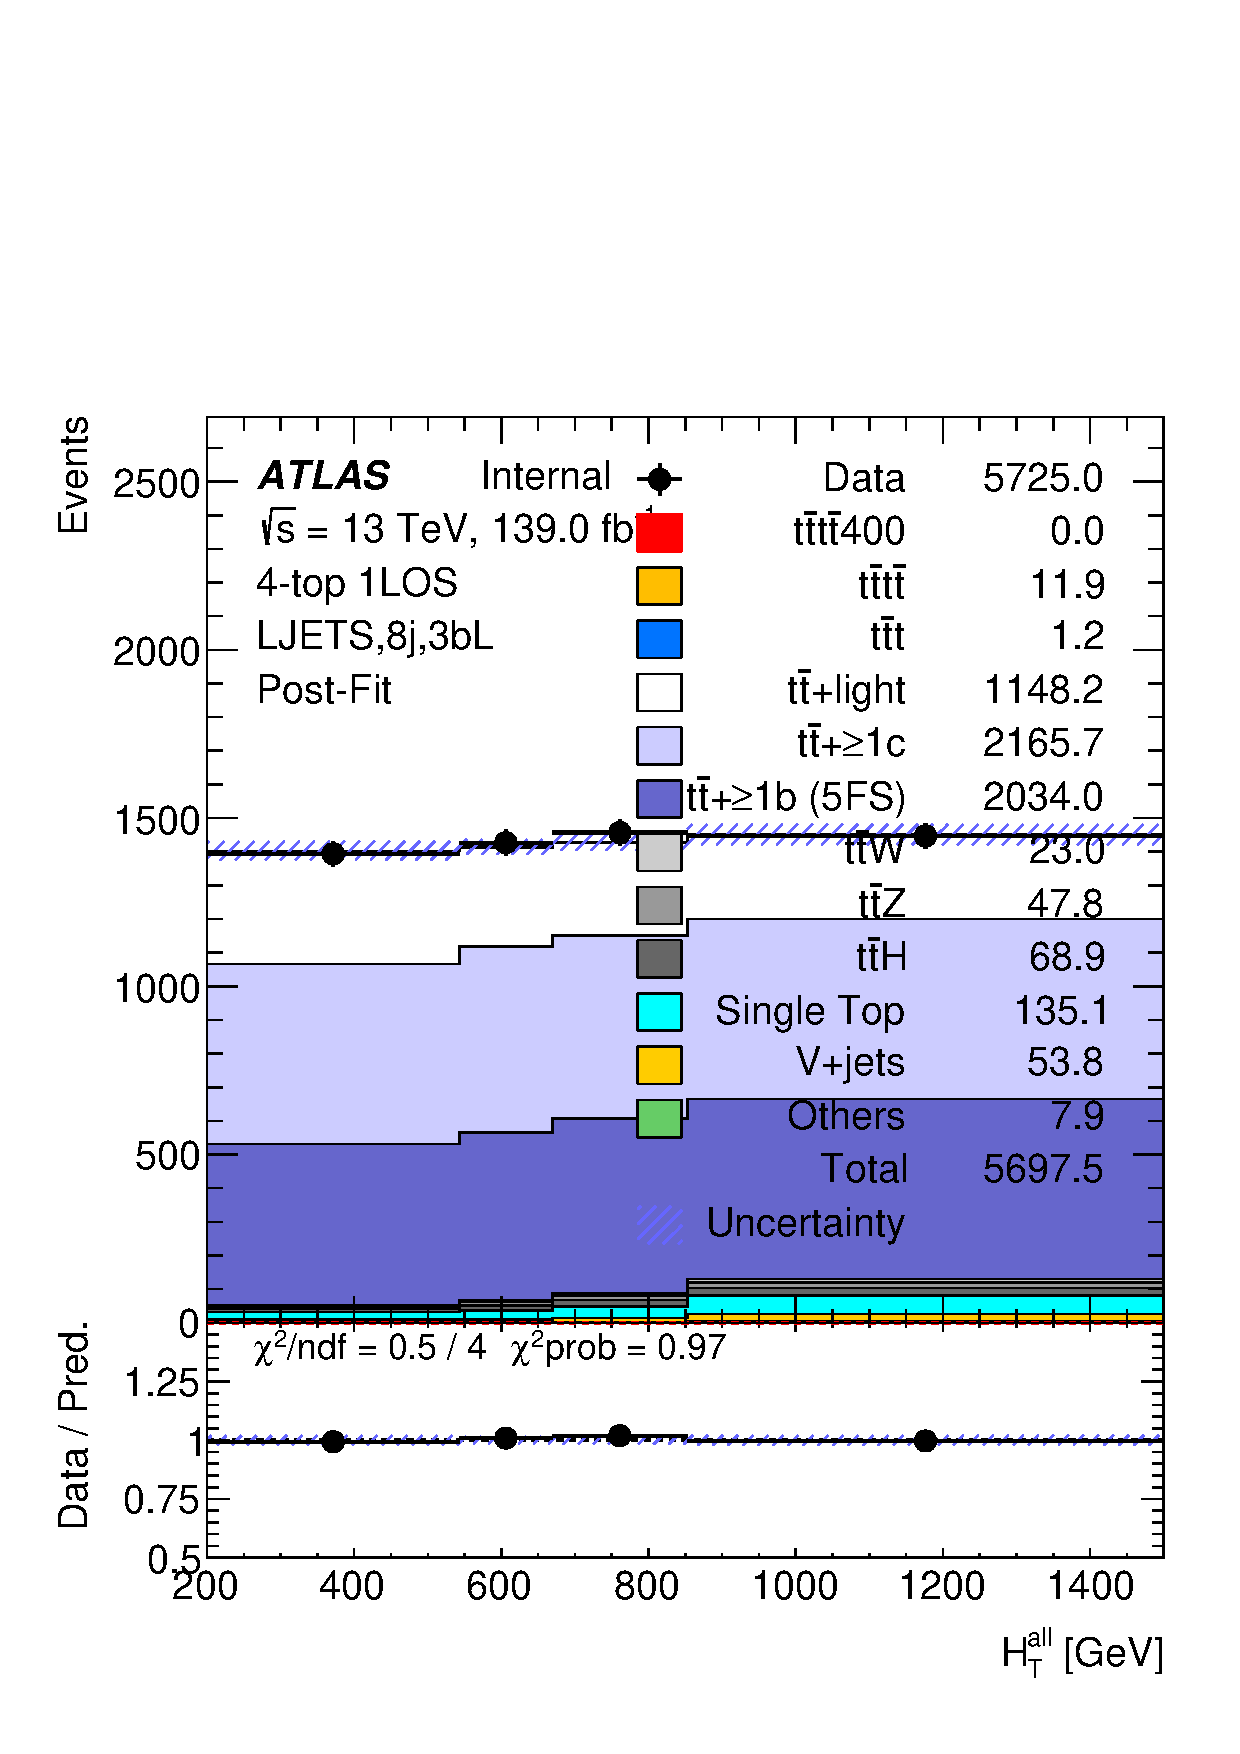
\includegraphics[width=0.23 \textwidth]{figures/fits/GNN/400/all/data_unblindedBonly/Plots/ljets_8j3bL_postFit.pdf} &
        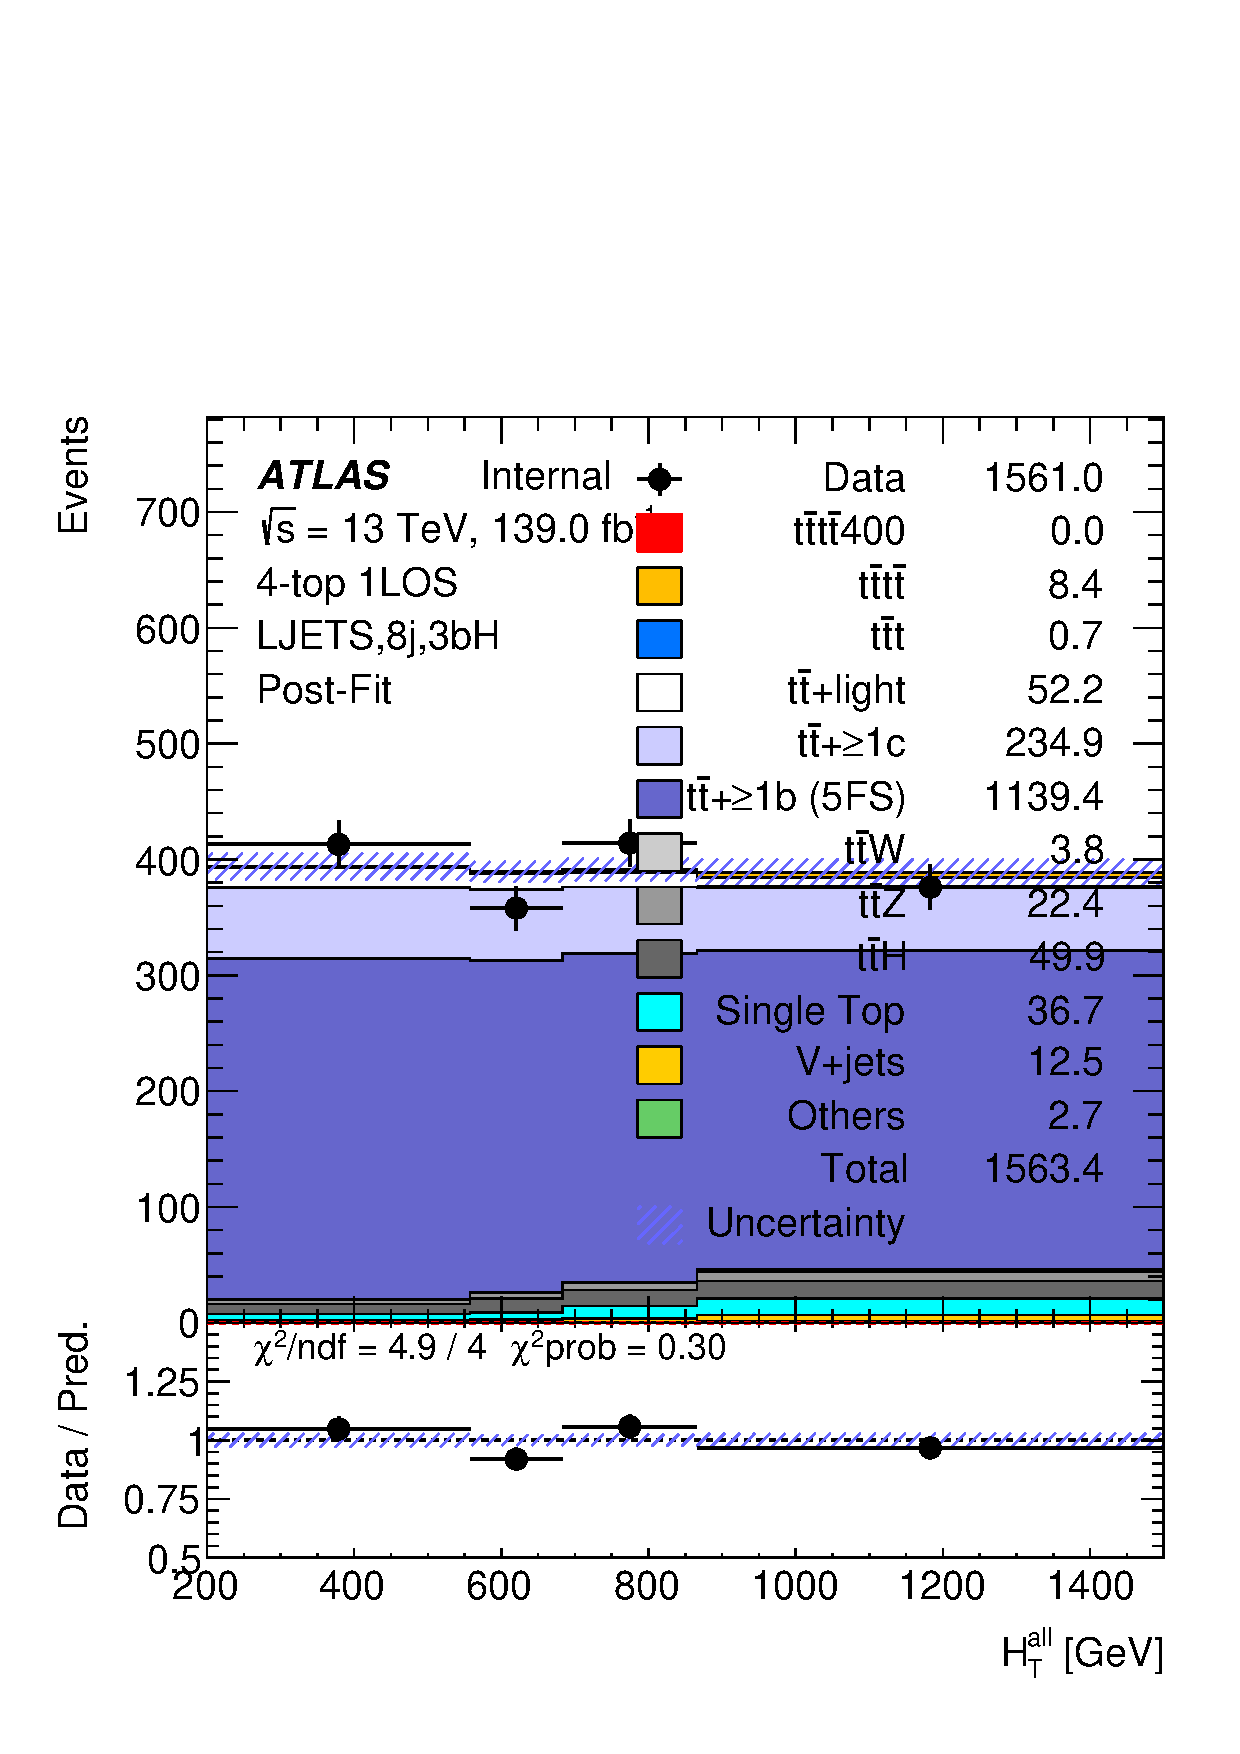
\includegraphics[width=0.23 \textwidth]{figures/fits/GNN/400/all/data_unblindedBonly/Plots/ljets_8j3bH_postFit.pdf} &
        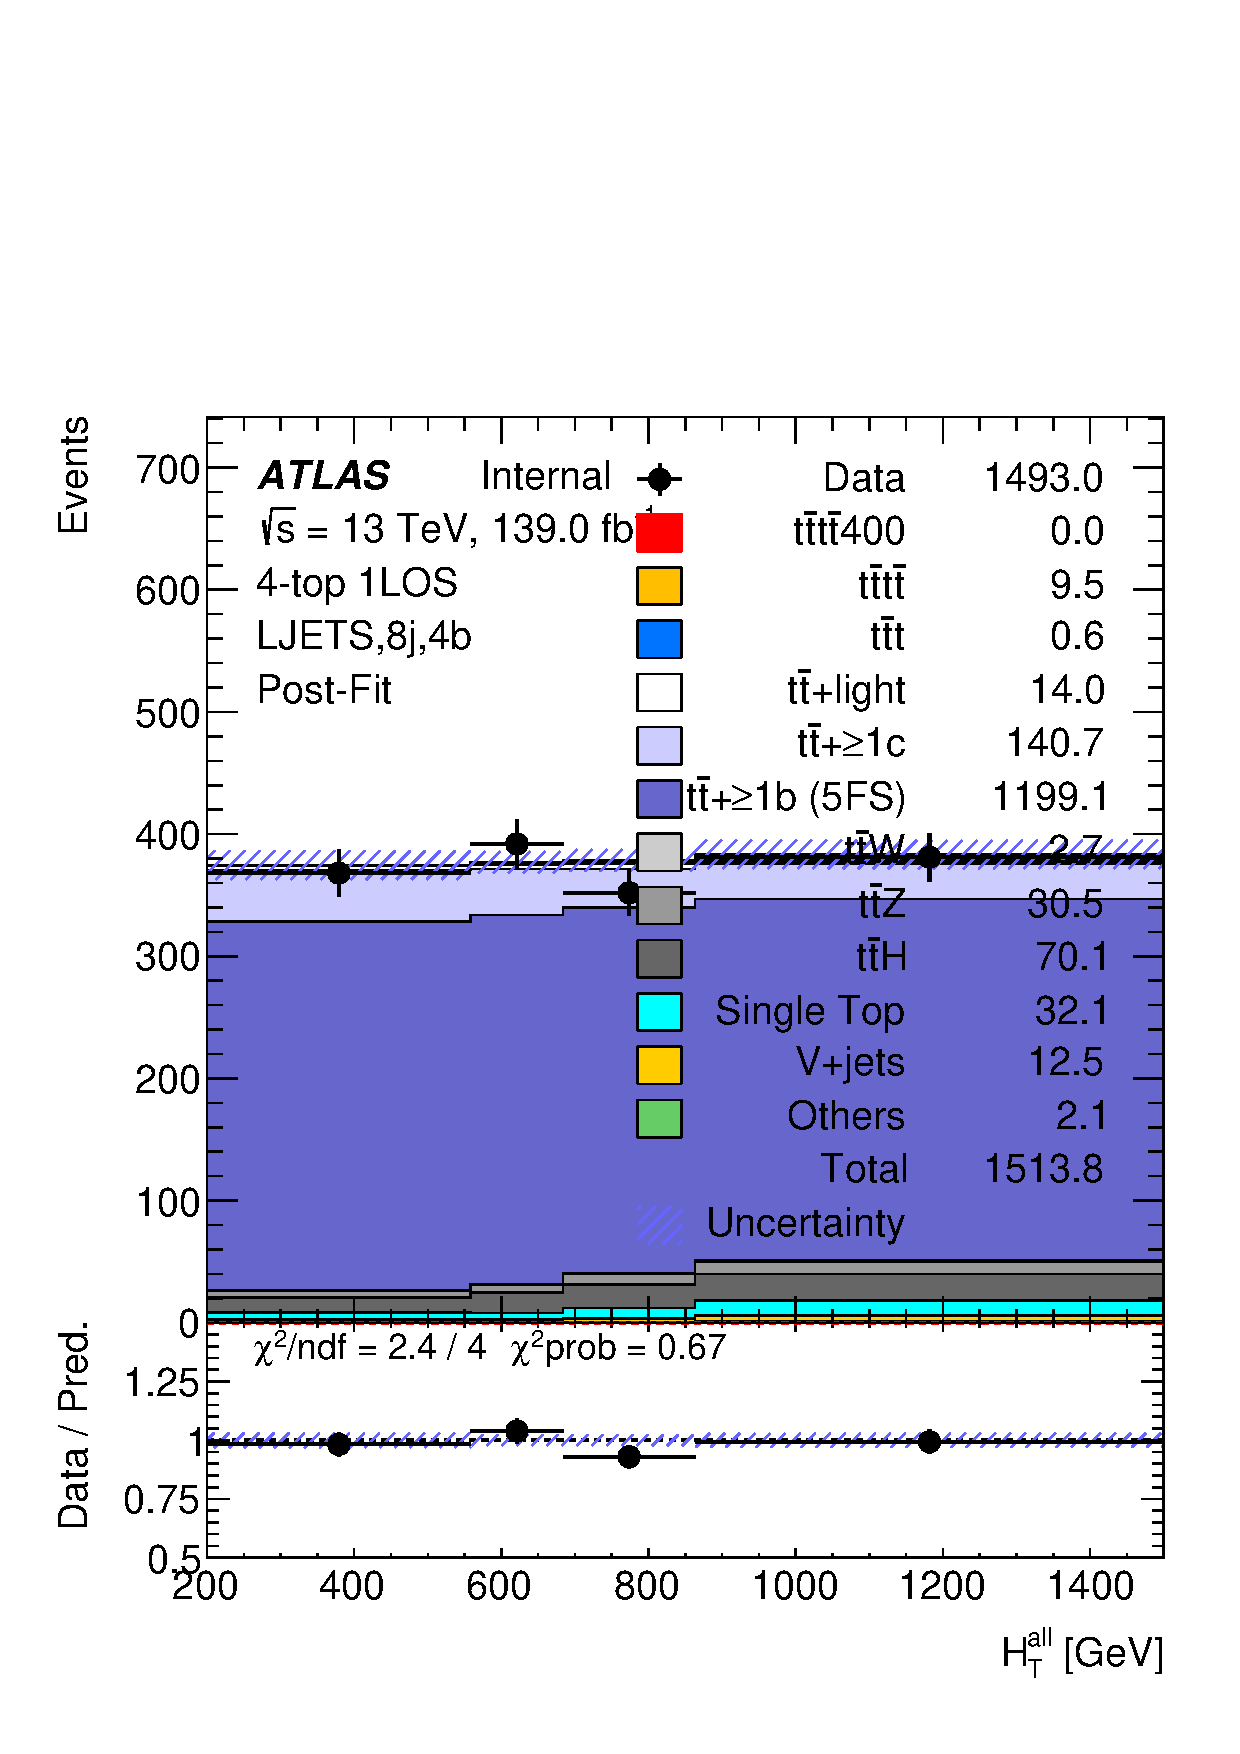
\includegraphics[width=0.23 \textwidth]{figures/fits/GNN/400/all/data_unblindedBonly/Plots/ljets_8j4b_postFit.pdf} &
        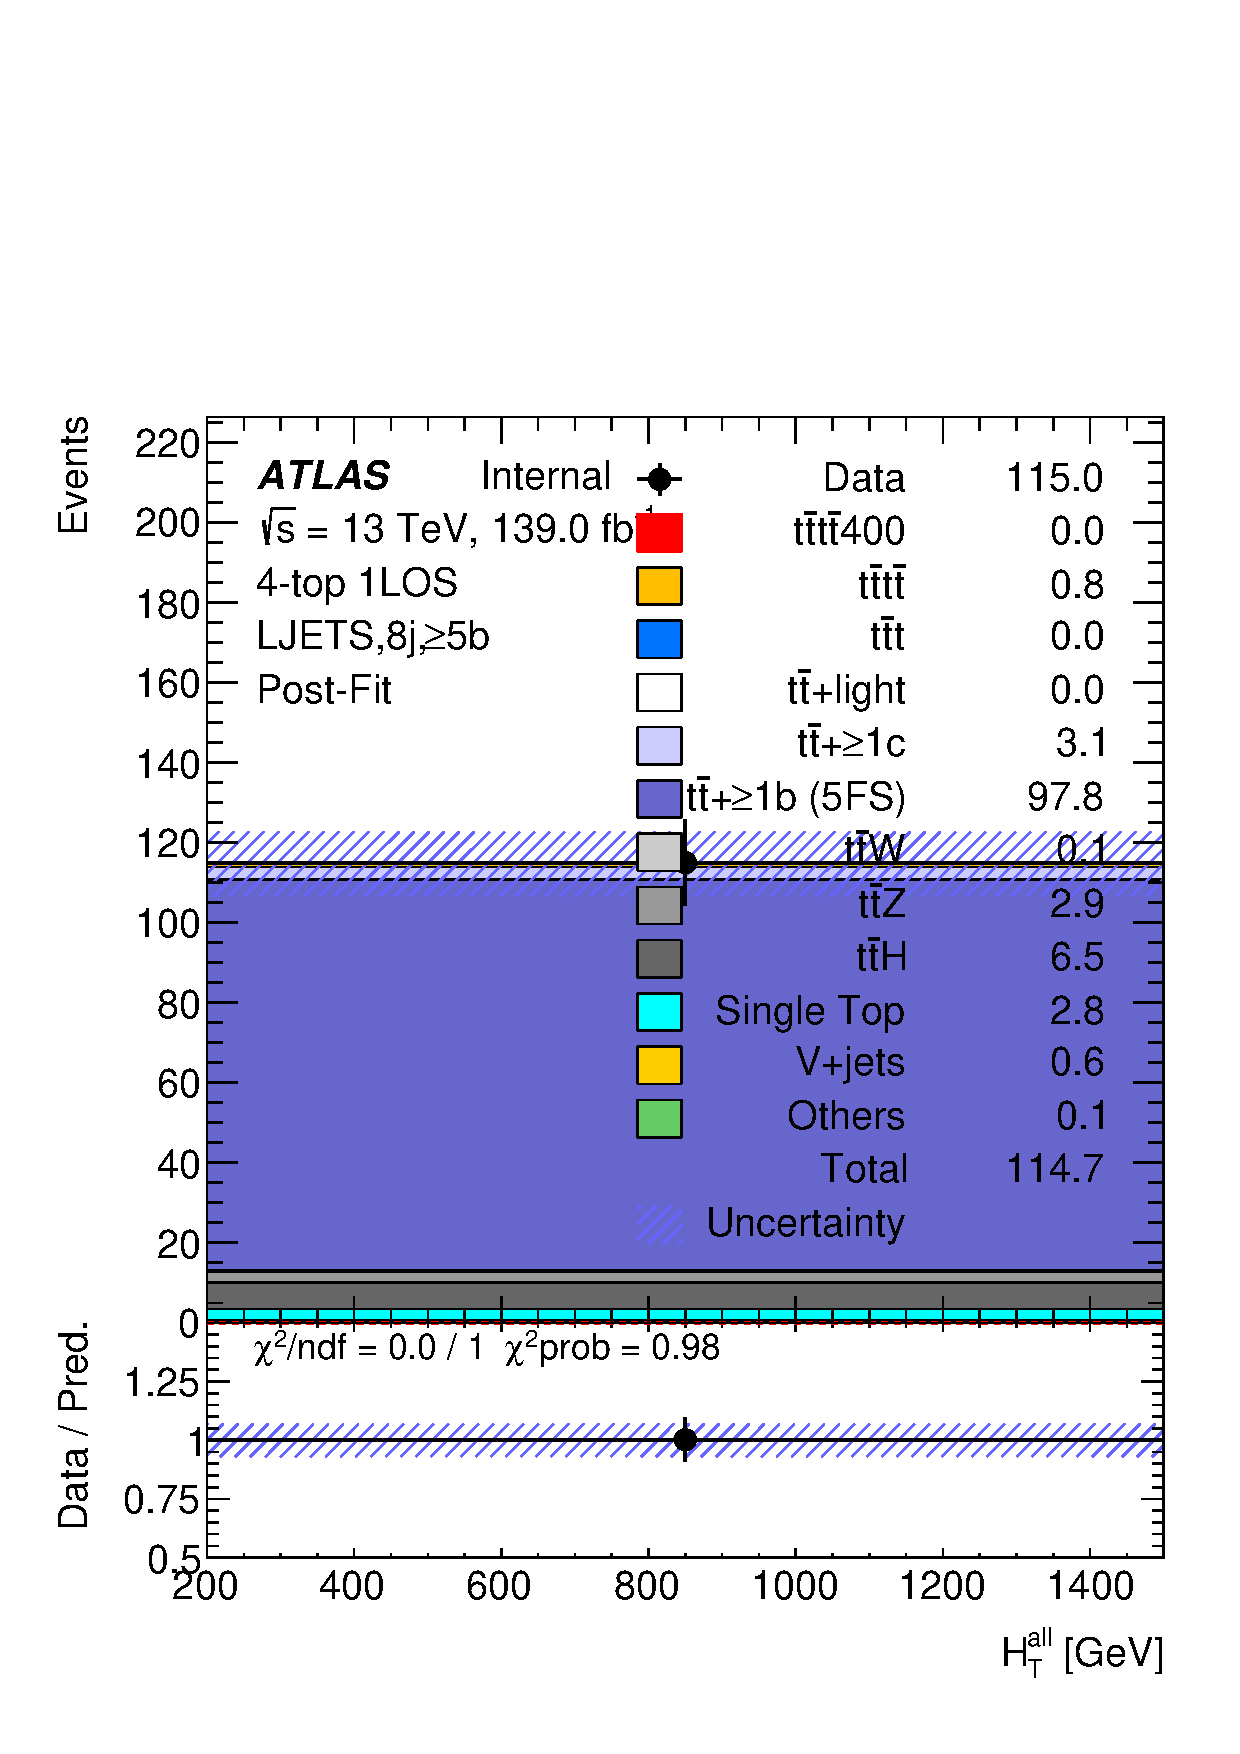
\includegraphics[width=0.23 \textwidth]{figures/fits/GNN/400/all/data_unblindedBonly/Plots/ljets_8jge5b_postFit.pdf}\\

        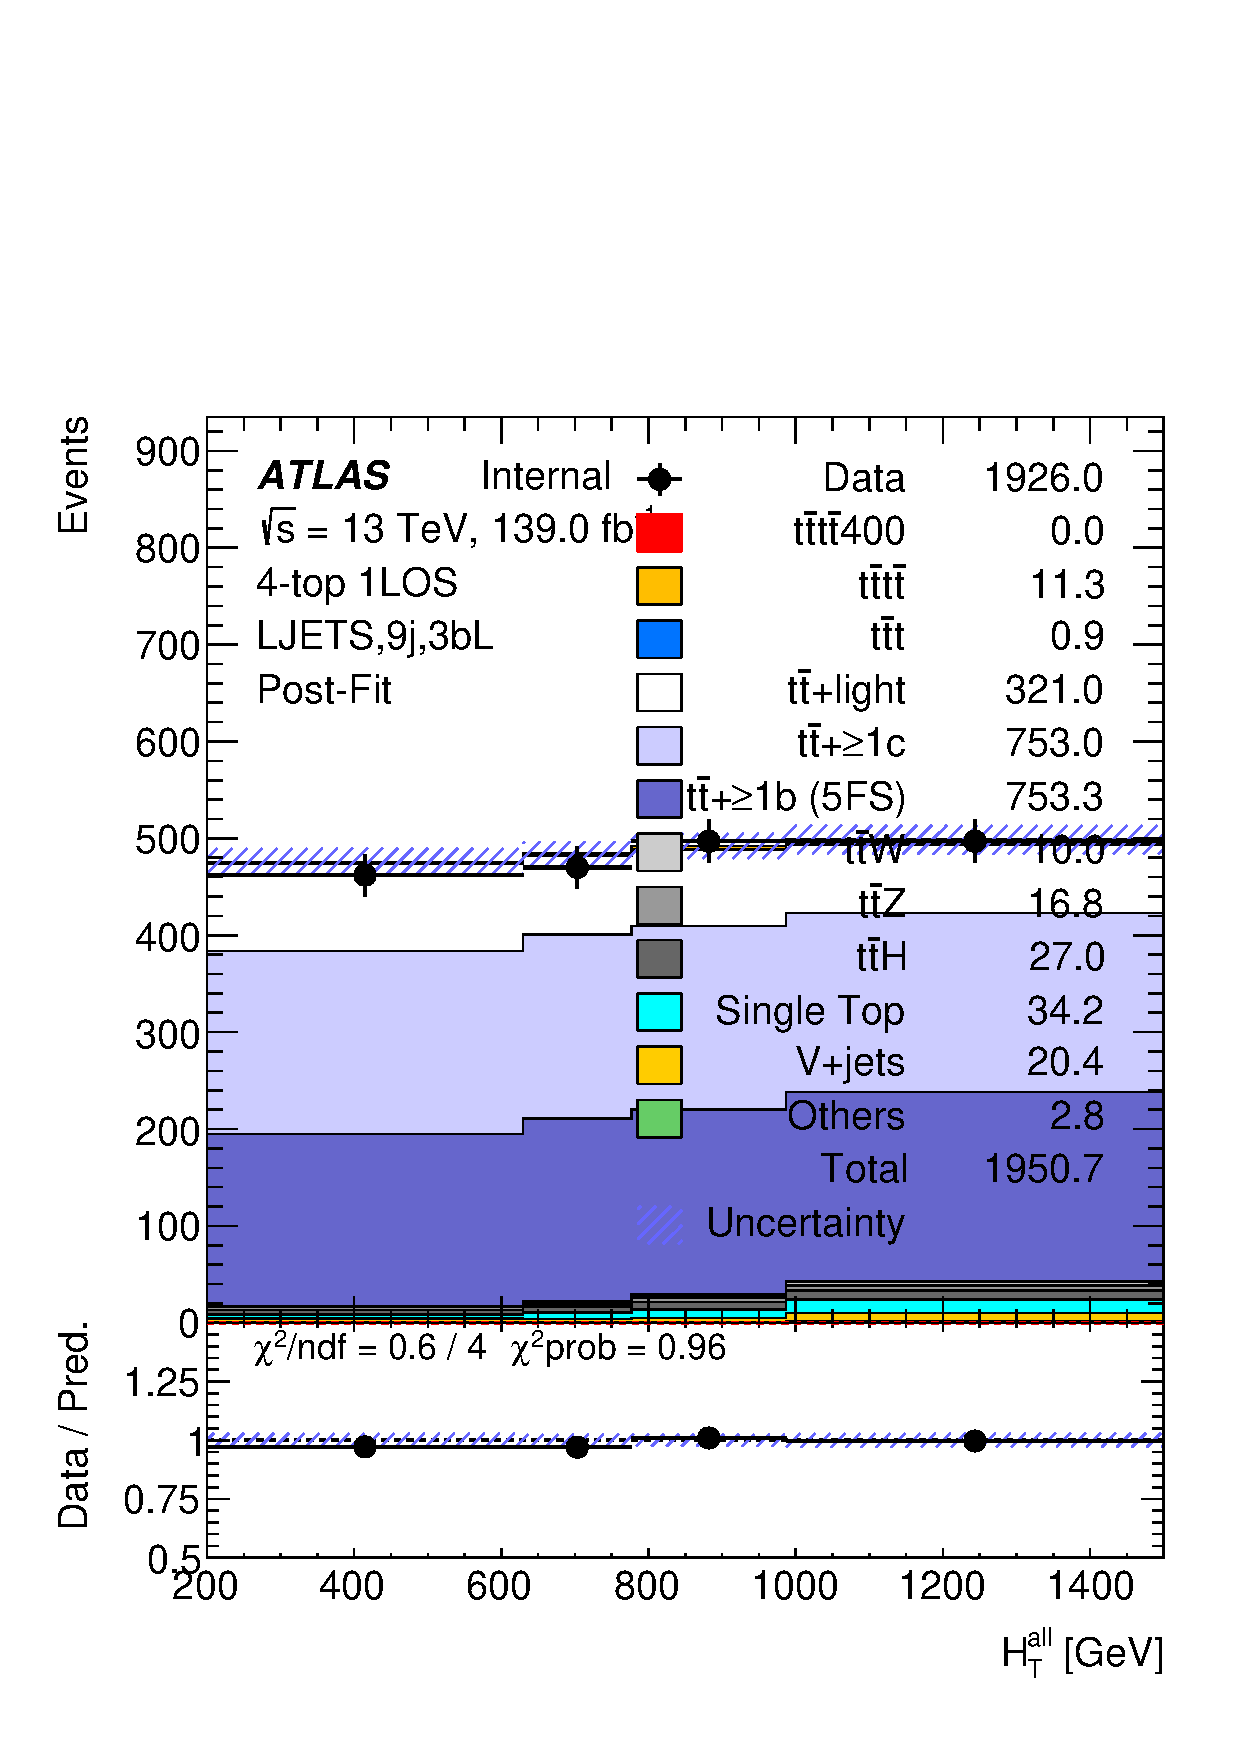
\includegraphics[width=0.23 \textwidth]{figures/fits/GNN/400/all/data_unblindedBonly/Plots/ljets_9j3bL_postFit.pdf} &
        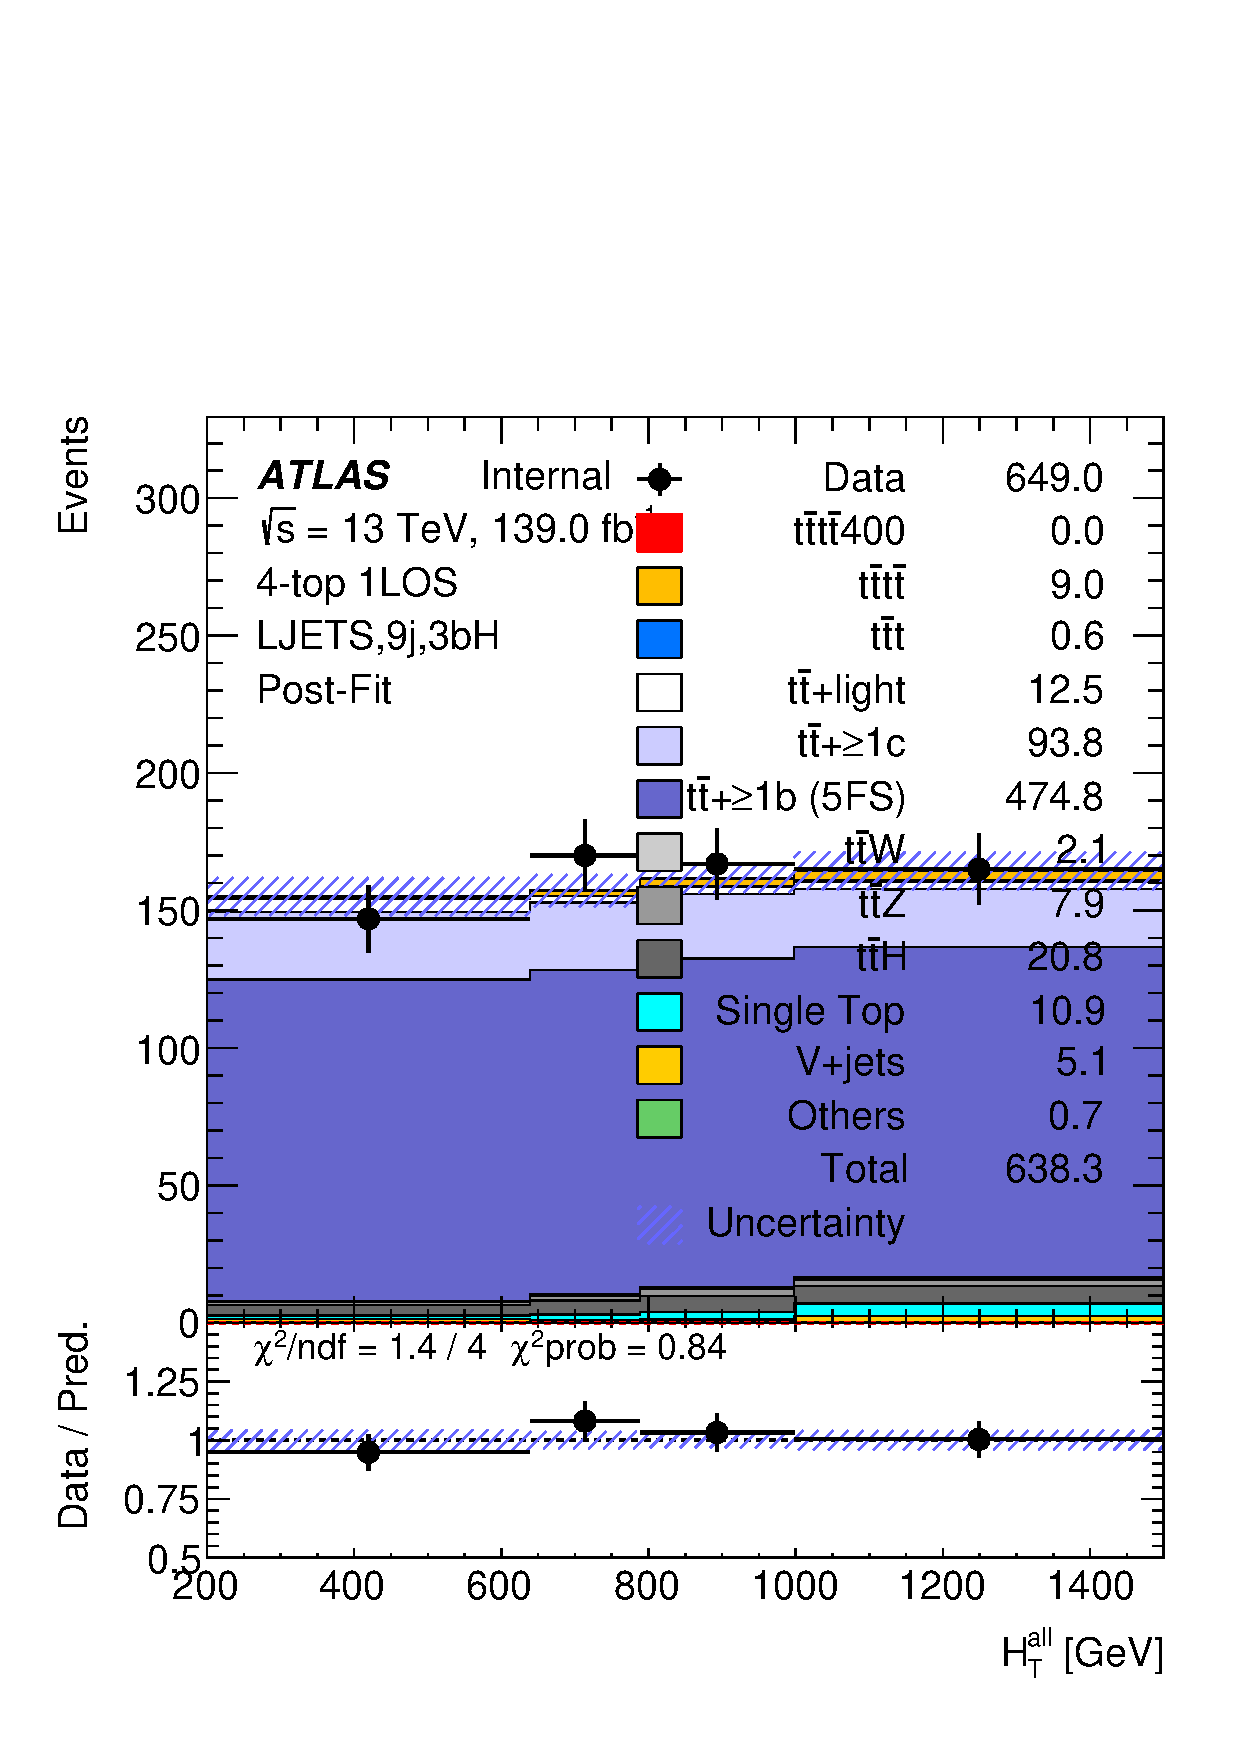
\includegraphics[width=0.23 \textwidth]{figures/fits/GNN/400/all/data_unblindedBonly/Plots/ljets_9j3bH_postFit.pdf} &
        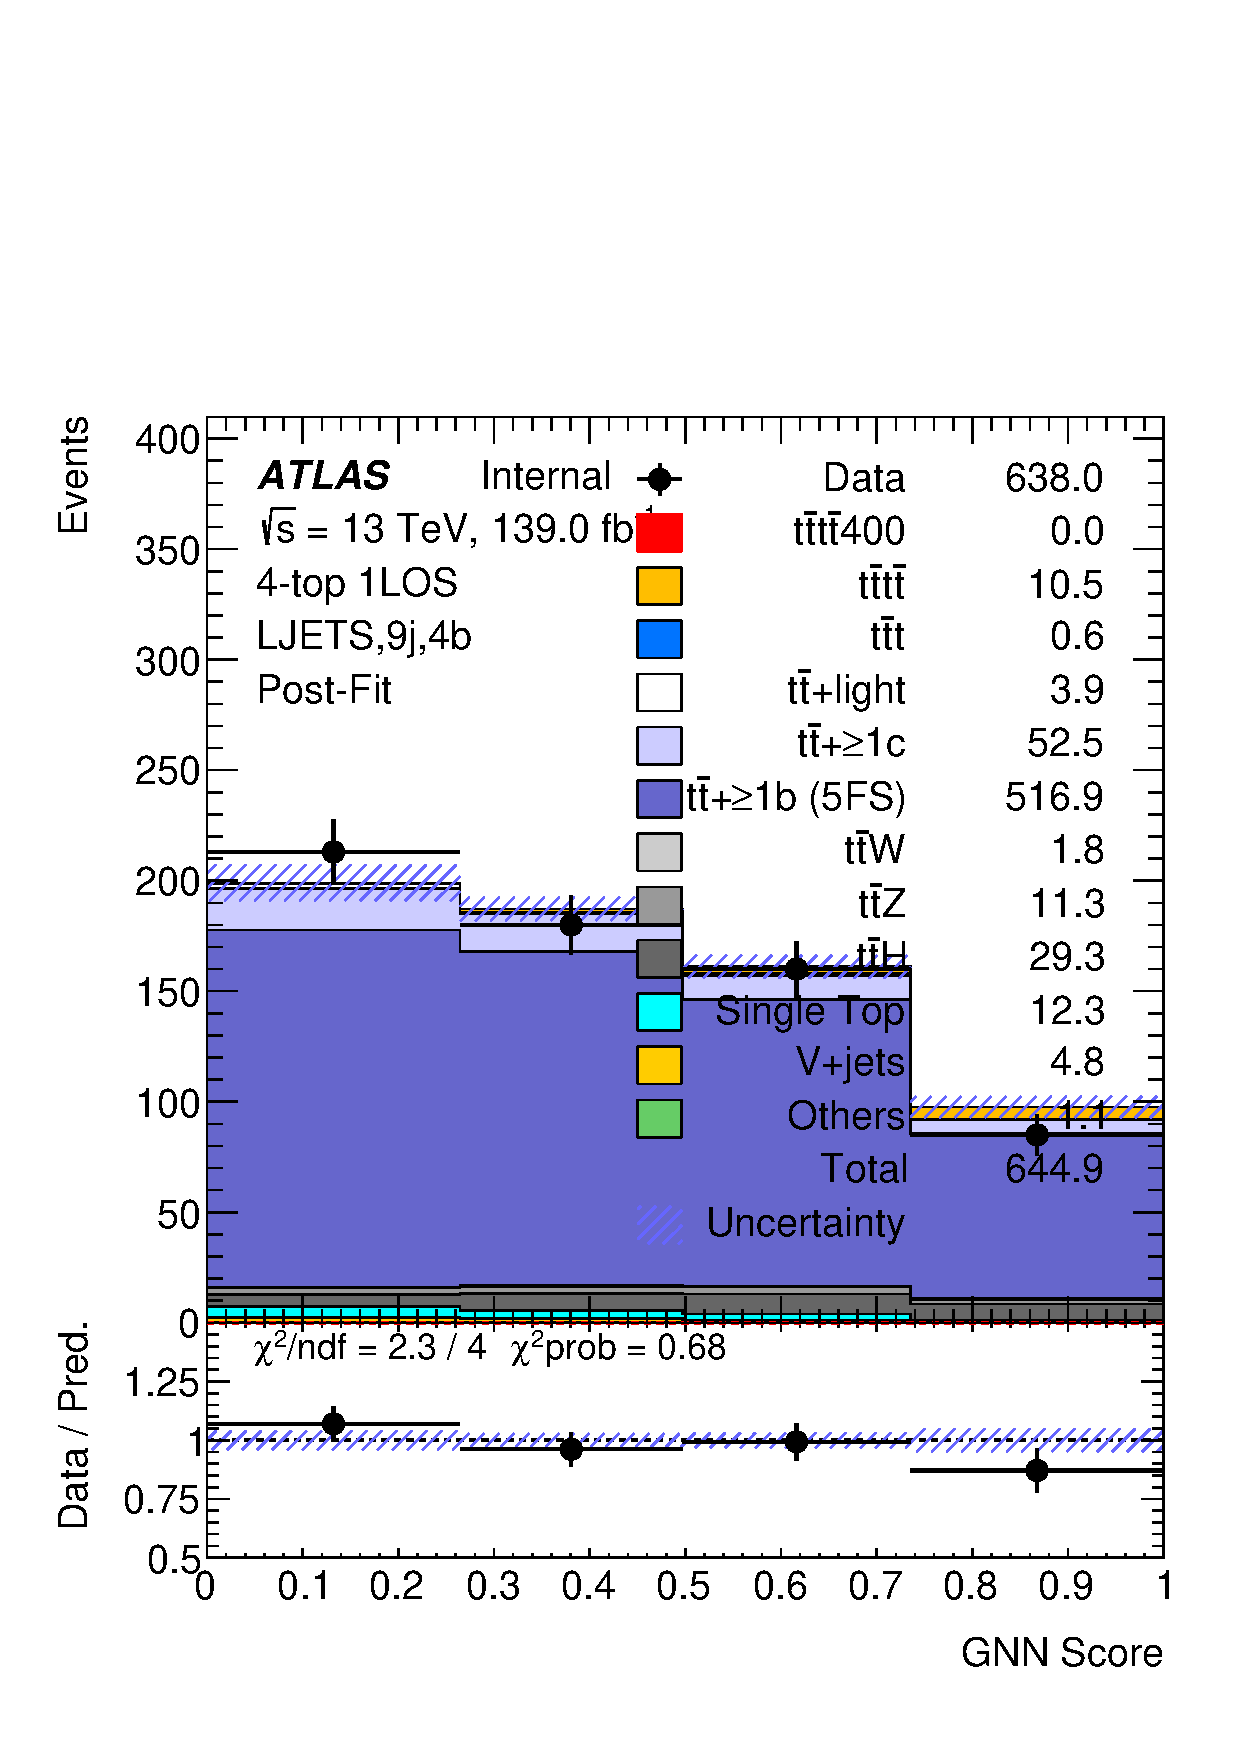
\includegraphics[width=0.23 \textwidth]{figures/fits/GNN/400/all/data_unblindedBonly/Plots/ljets_9j4b_postFit.pdf} &
        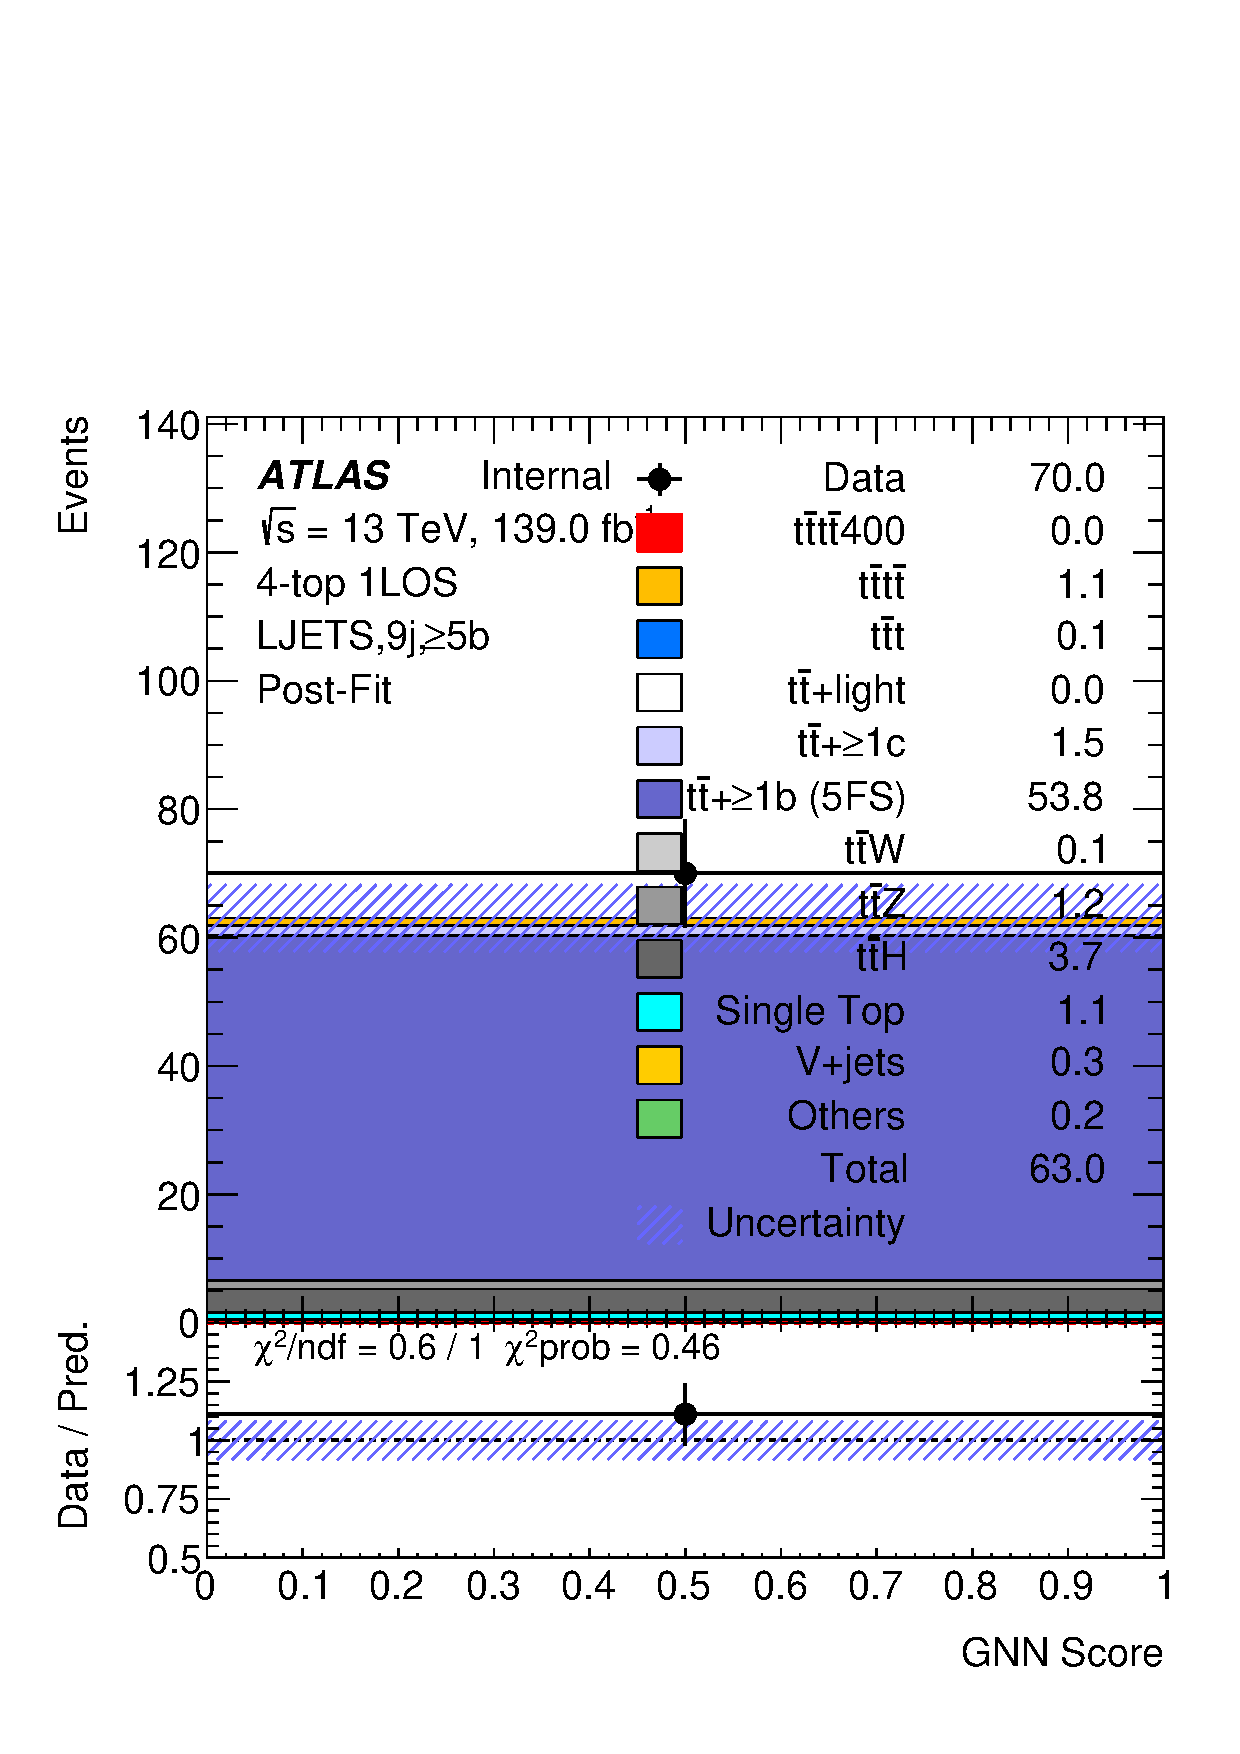
\includegraphics[width=0.23 \textwidth]{figures/fits/GNN/400/all/data_unblindedBonly/Plots/ljets_9jge5b_postFit.pdf} \\

        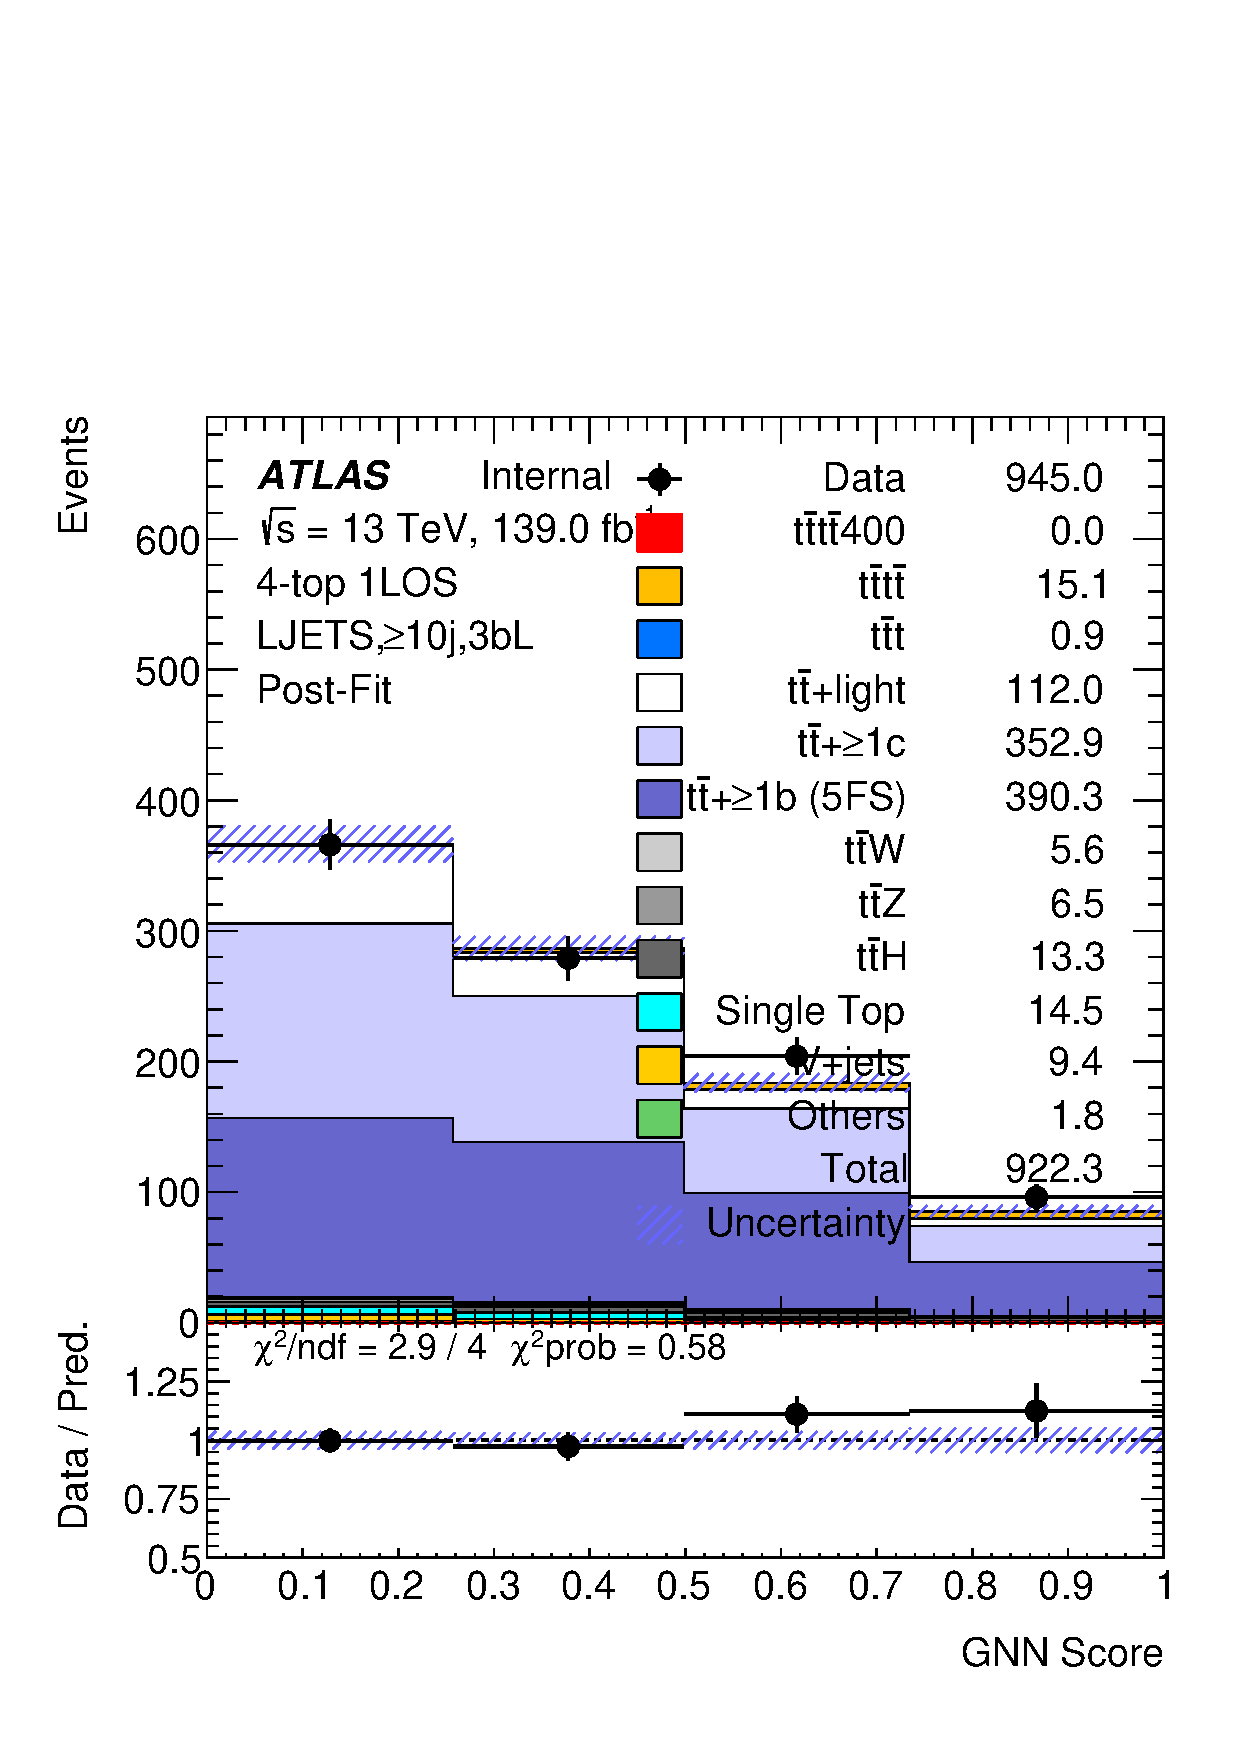
\includegraphics[width=0.23 \textwidth]{figures/fits/GNN/400/all/data_unblindedBonly/Plots/ljets_ge10j3bL_postFit.pdf} &
        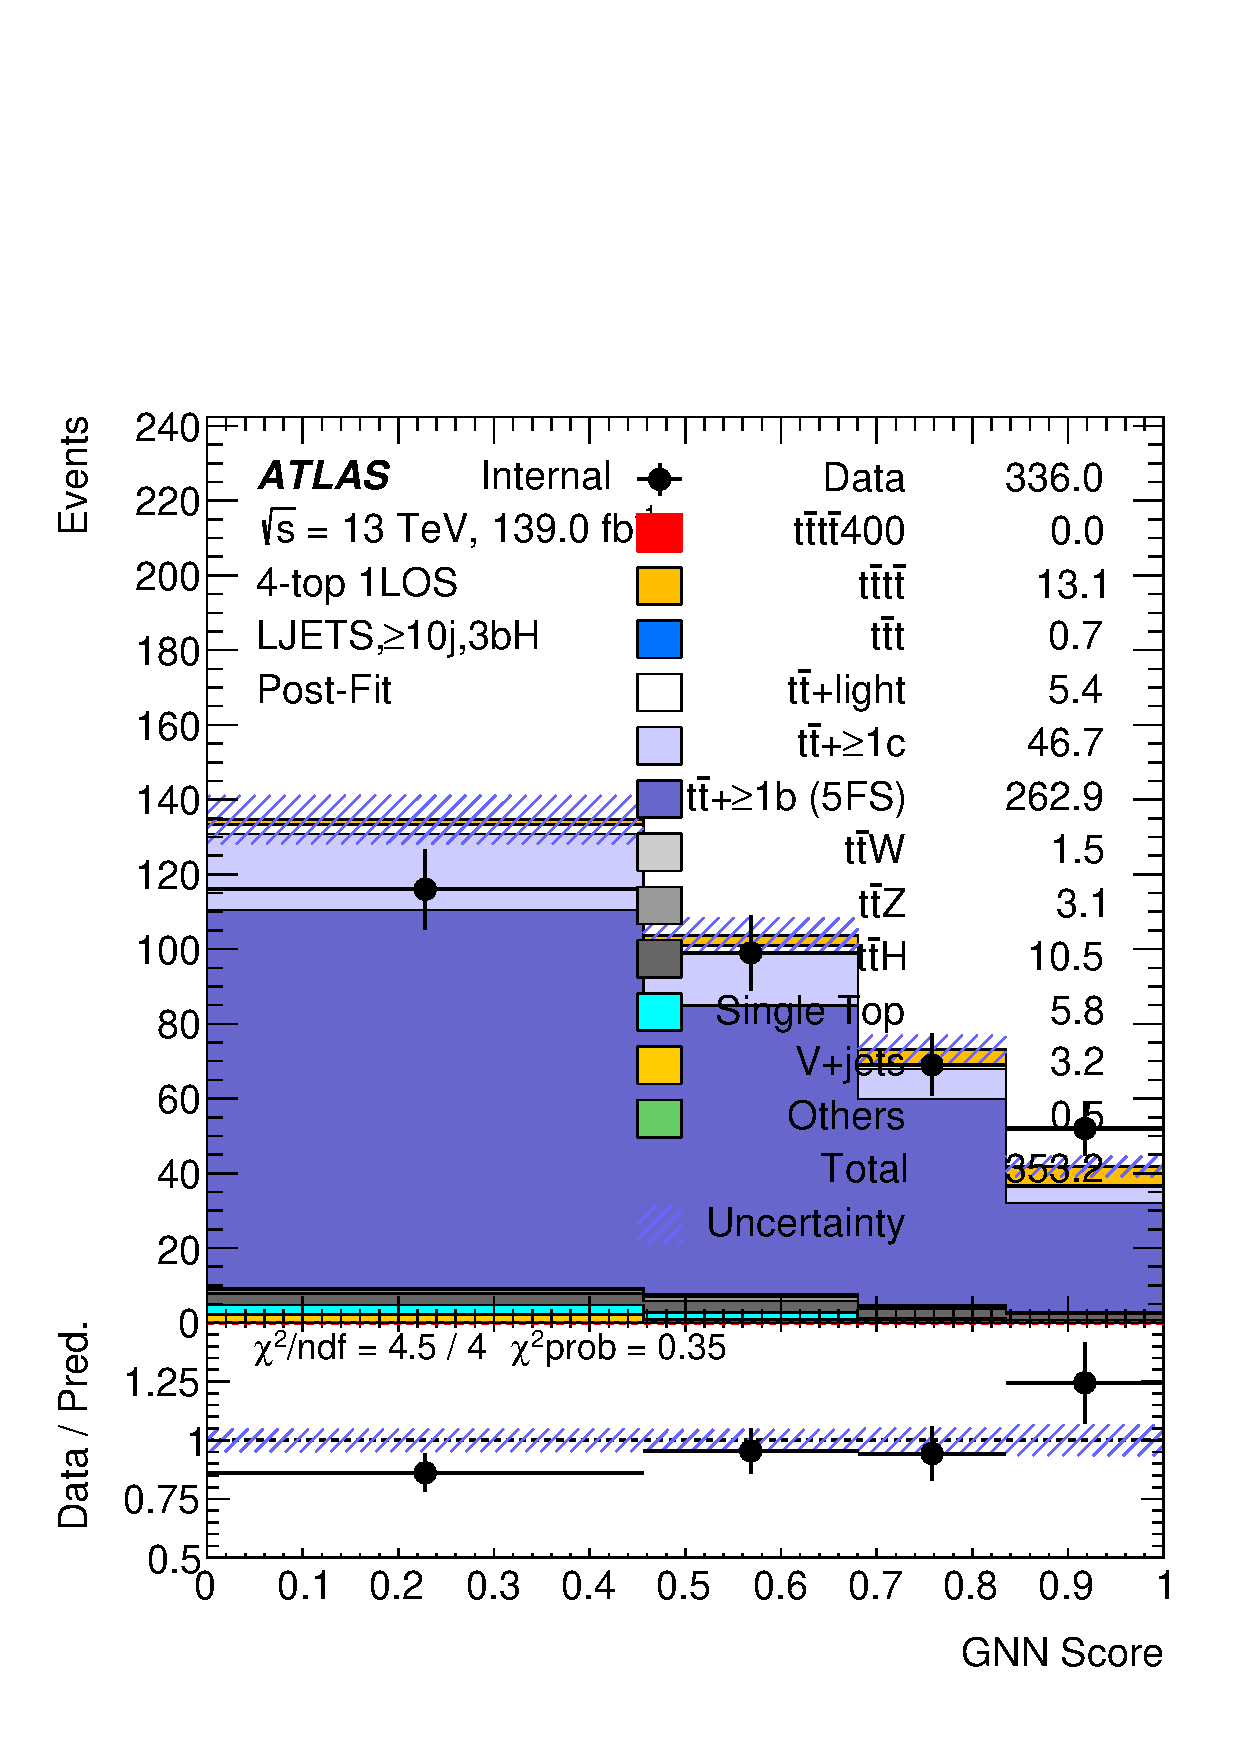
\includegraphics[width=0.23 \textwidth]{figures/fits/GNN/400/all/data_unblindedBonly/Plots/ljets_ge10j3bH_postFit.pdf} &
        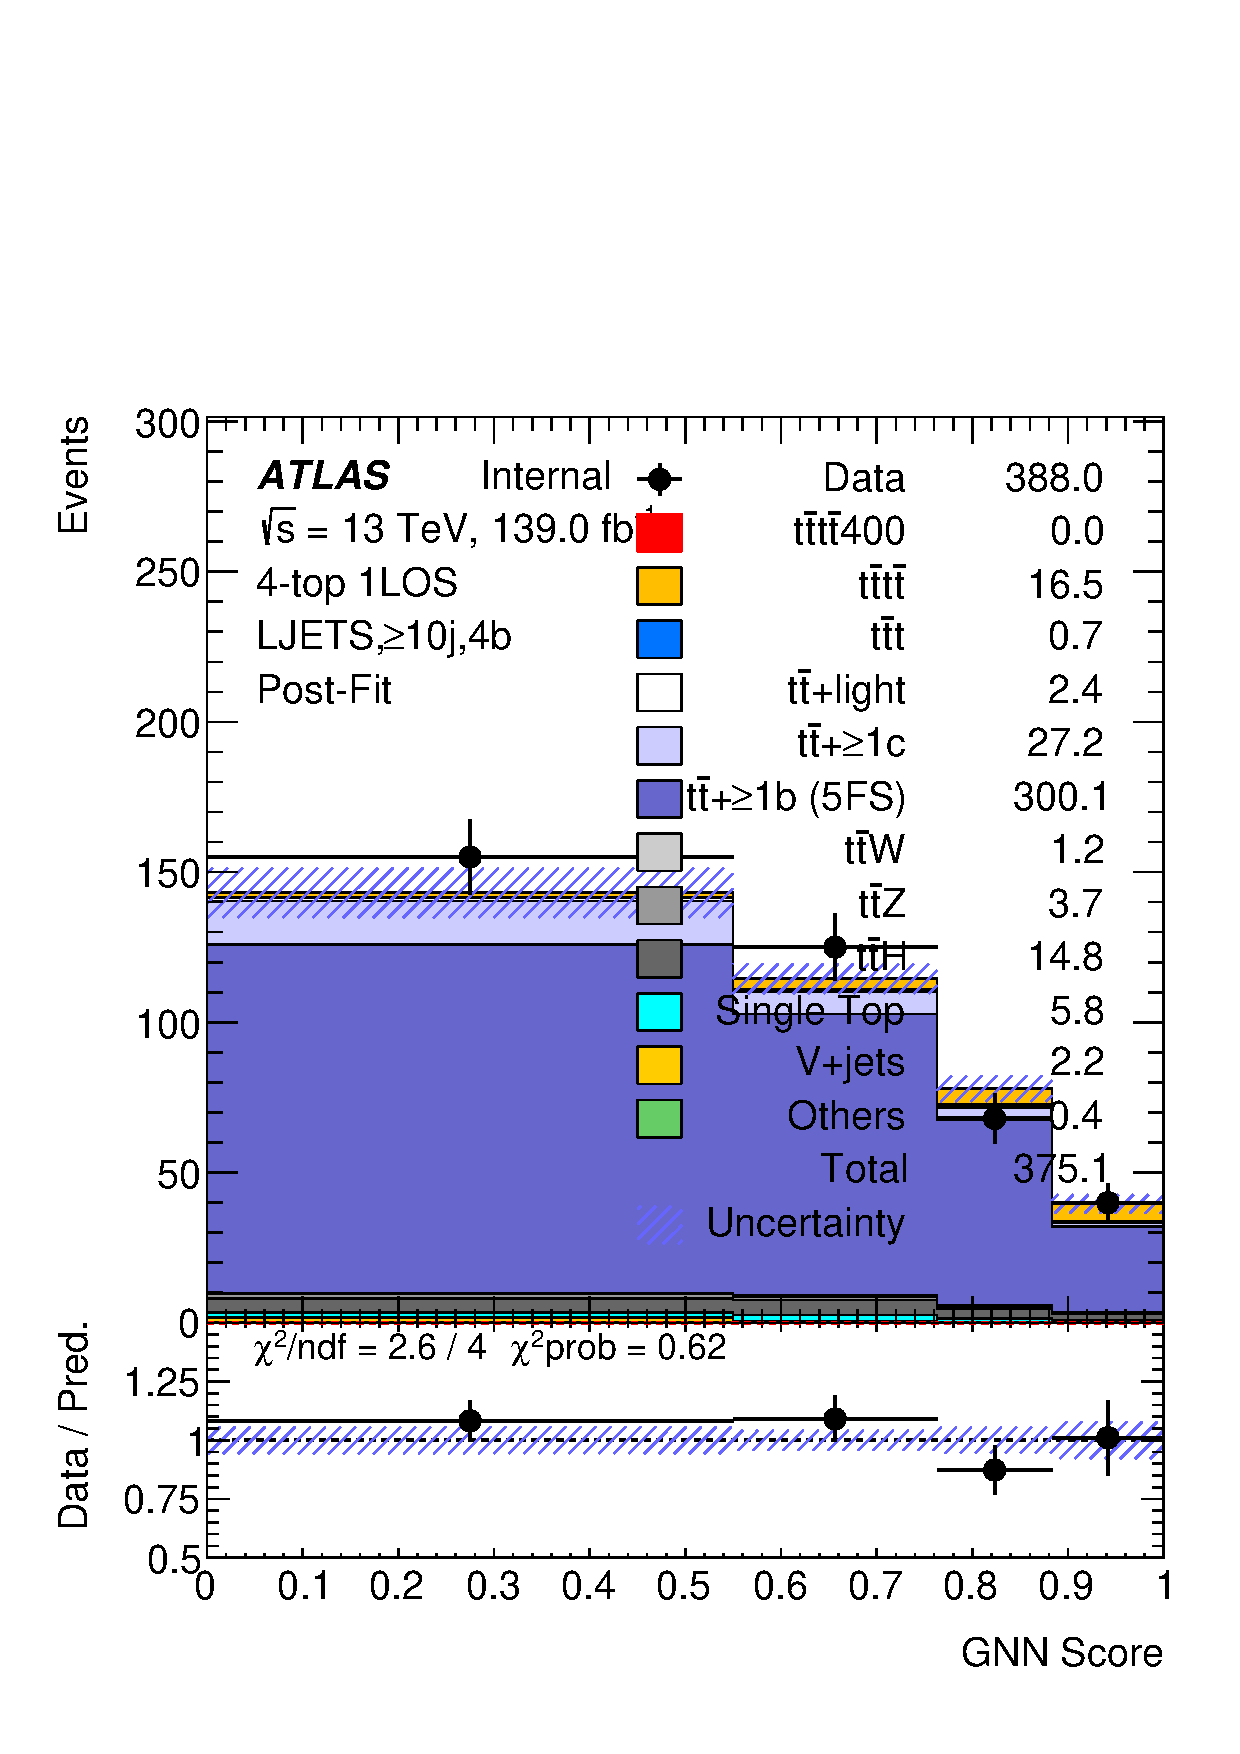
\includegraphics[width=0.23 \textwidth]{figures/fits/GNN/400/all/data_unblindedBonly/Plots/ljets_ge10j4b_postFit.pdf} &
        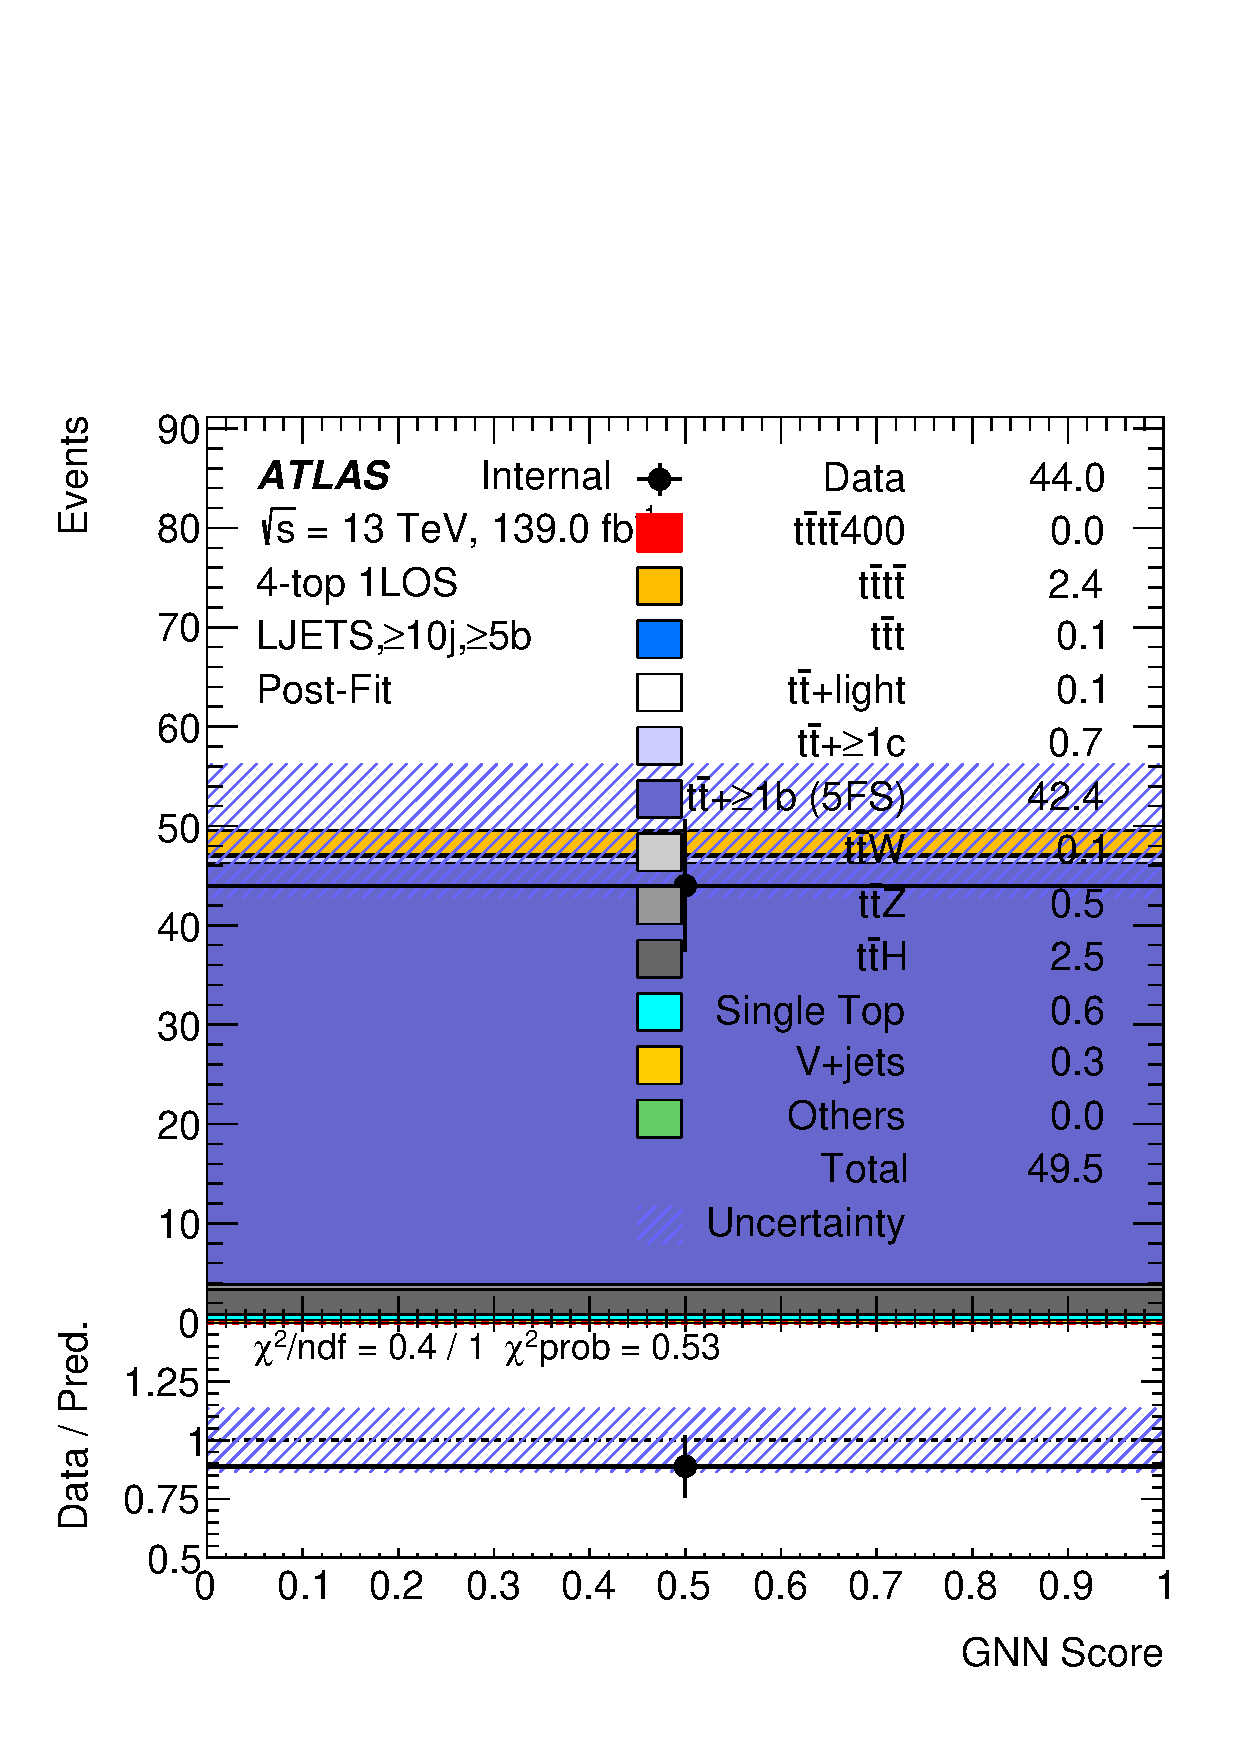
\includegraphics[width=0.23 \textwidth]{figures/fits/GNN/400/all/data_unblindedBonly/Plots/ljets_ge10jge5b_postFit.pdf} \\
        \end{tabular}
        \caption{\label{fig:unblinded_data_Bonly_postfit_1L}Post-fit distributions for 1L regions obtained with background-only unblinded data fit, compared with data yields for mH = 400 GeV. The fit is done using all regions (1L+2L).}
\end{center}
\end{figure}

\begin{figure}[htbp!]
        \begin{center} \setlength{\tabcolsep}{2.5pt}\footnotesize
        \begin{tabular}{ccc}
        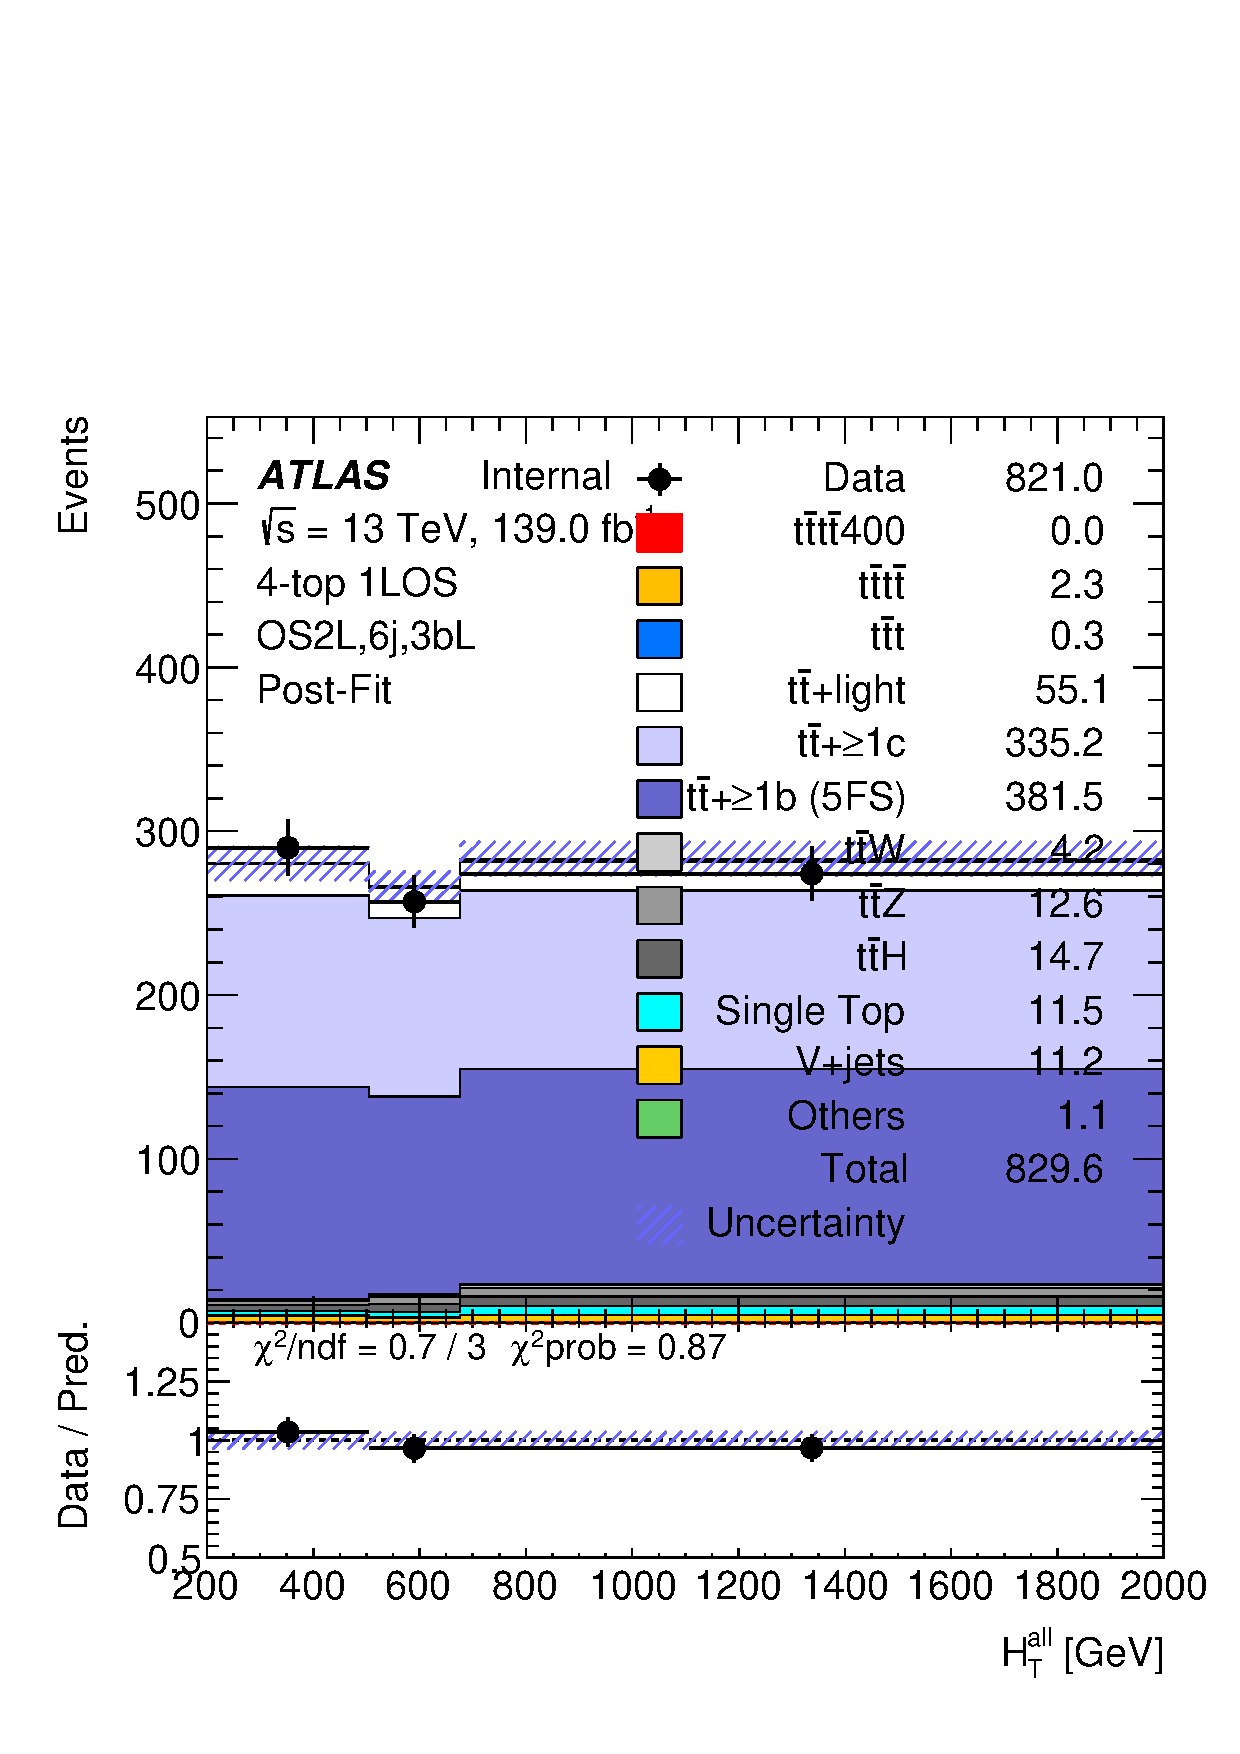
\includegraphics[width=0.31 \textwidth]{figures/fits/GNN/400/all/data_unblindedBonly/Plots/os2l_6j3bL_postFit.pdf} &
        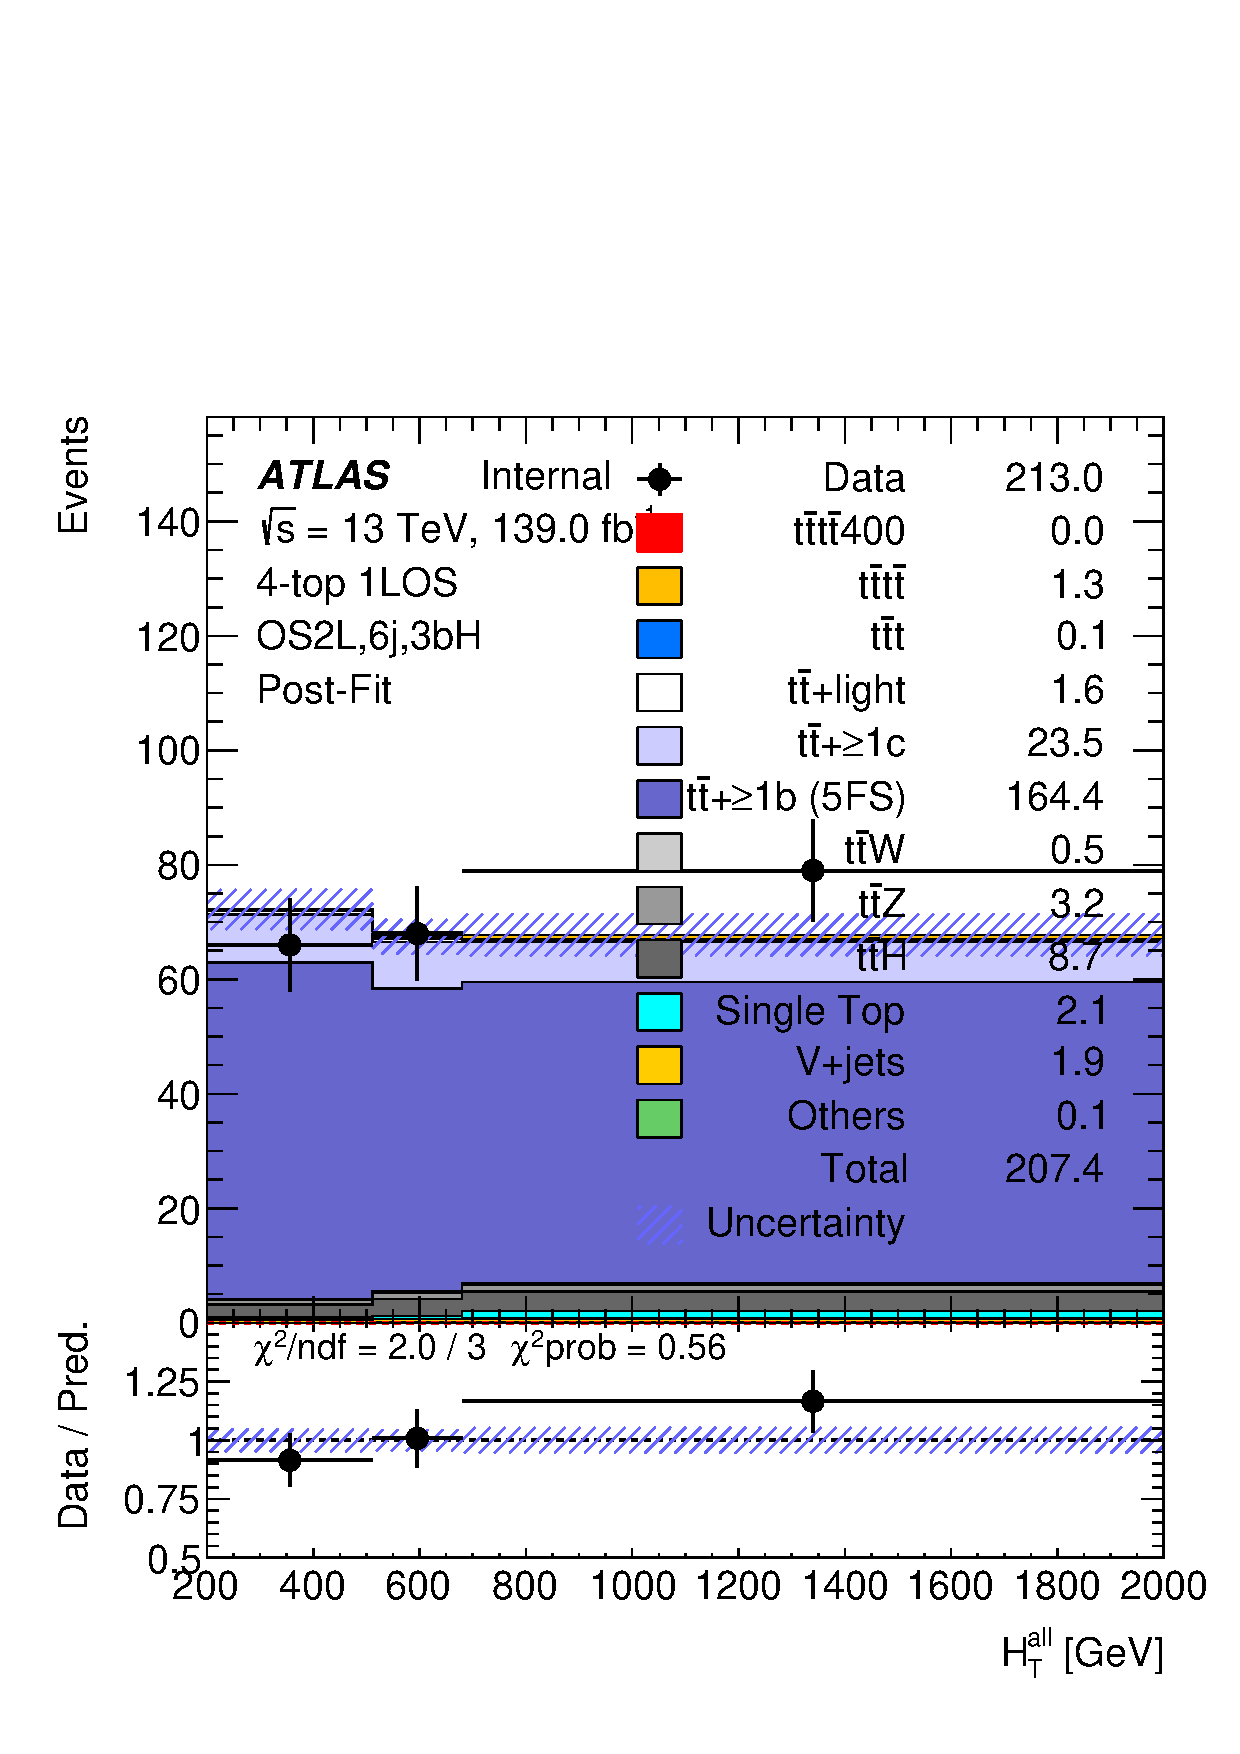
\includegraphics[width=0.31 \textwidth]{figures/fits/GNN/400/all/data_unblindedBonly/Plots/os2l_6j3bH_postFit.pdf} &
        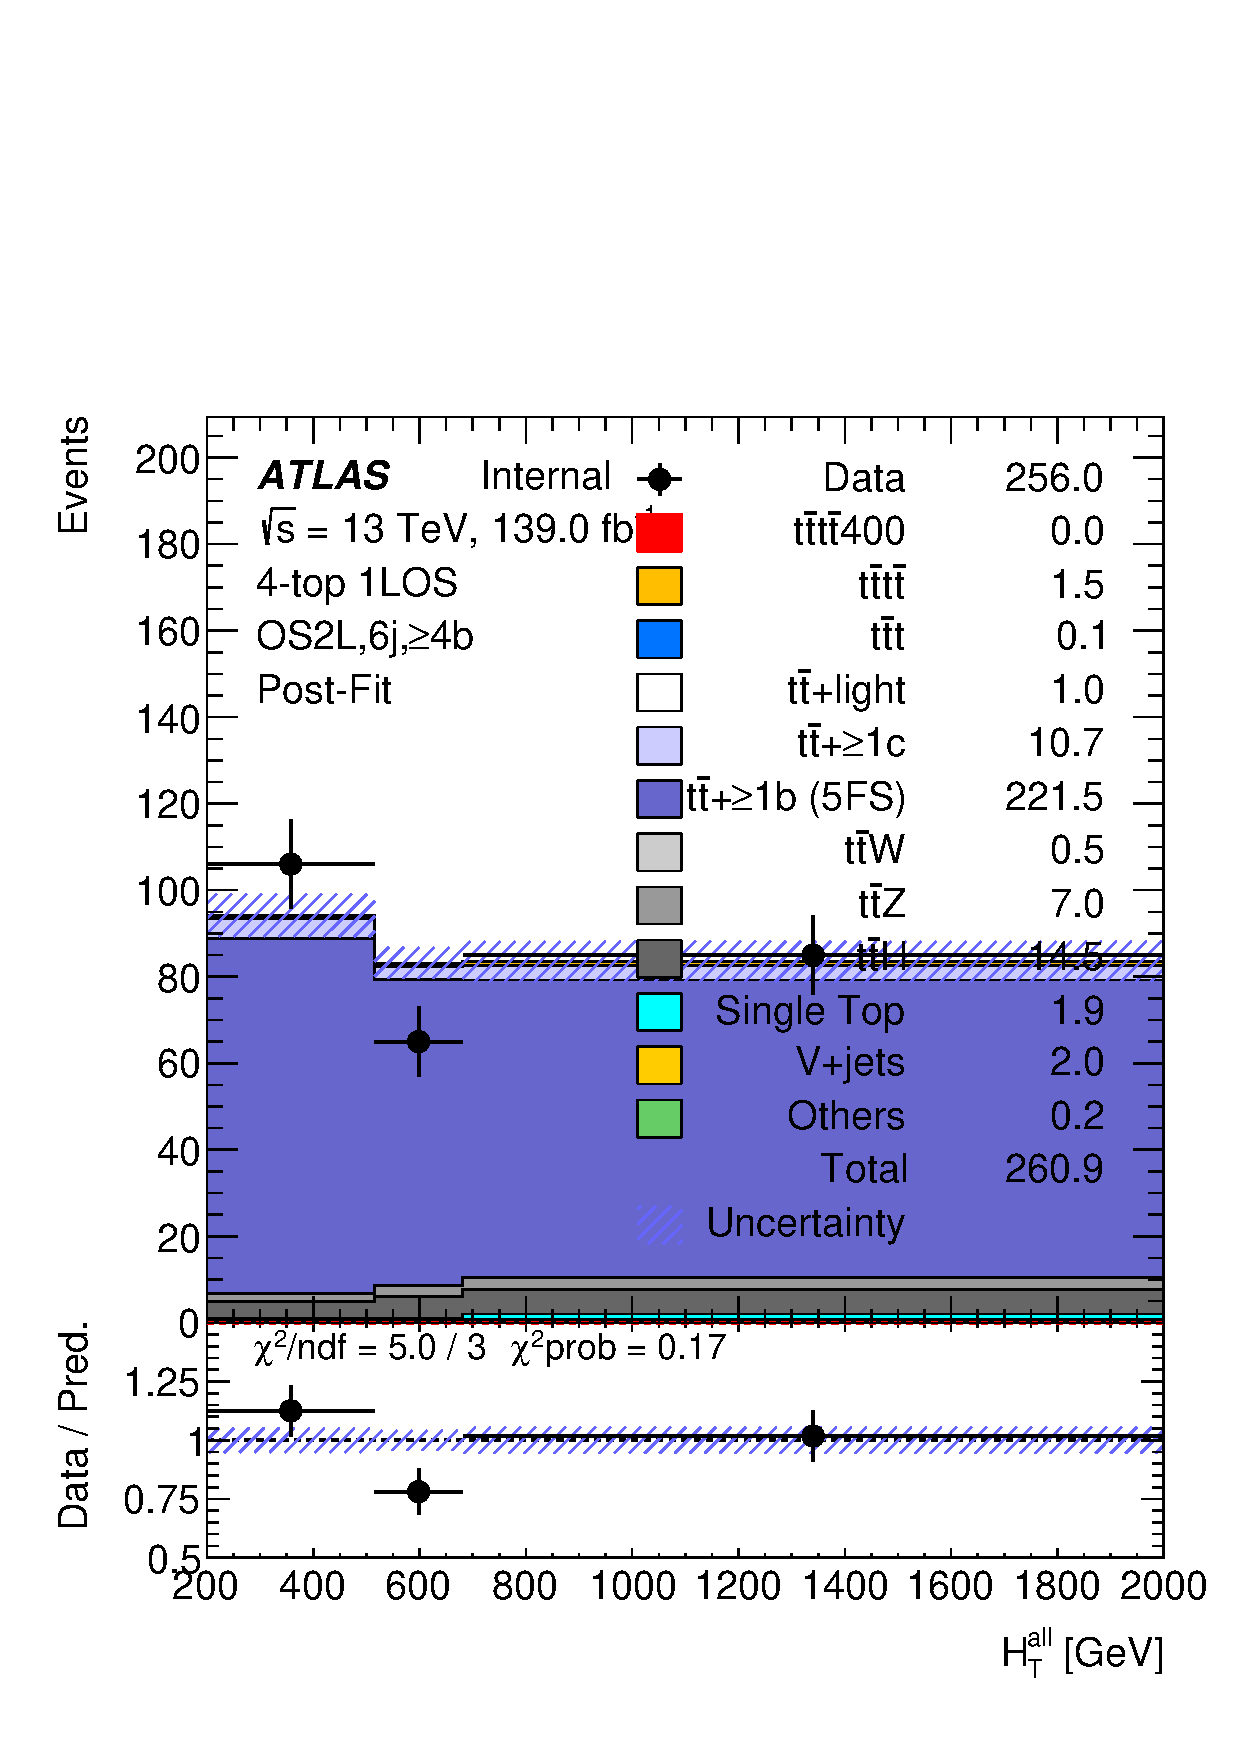
\includegraphics[width=0.31 \textwidth]{figures/fits/GNN/400/all/data_unblindedBonly/Plots/os2l_6jge4b_postFit.pdf} \\

        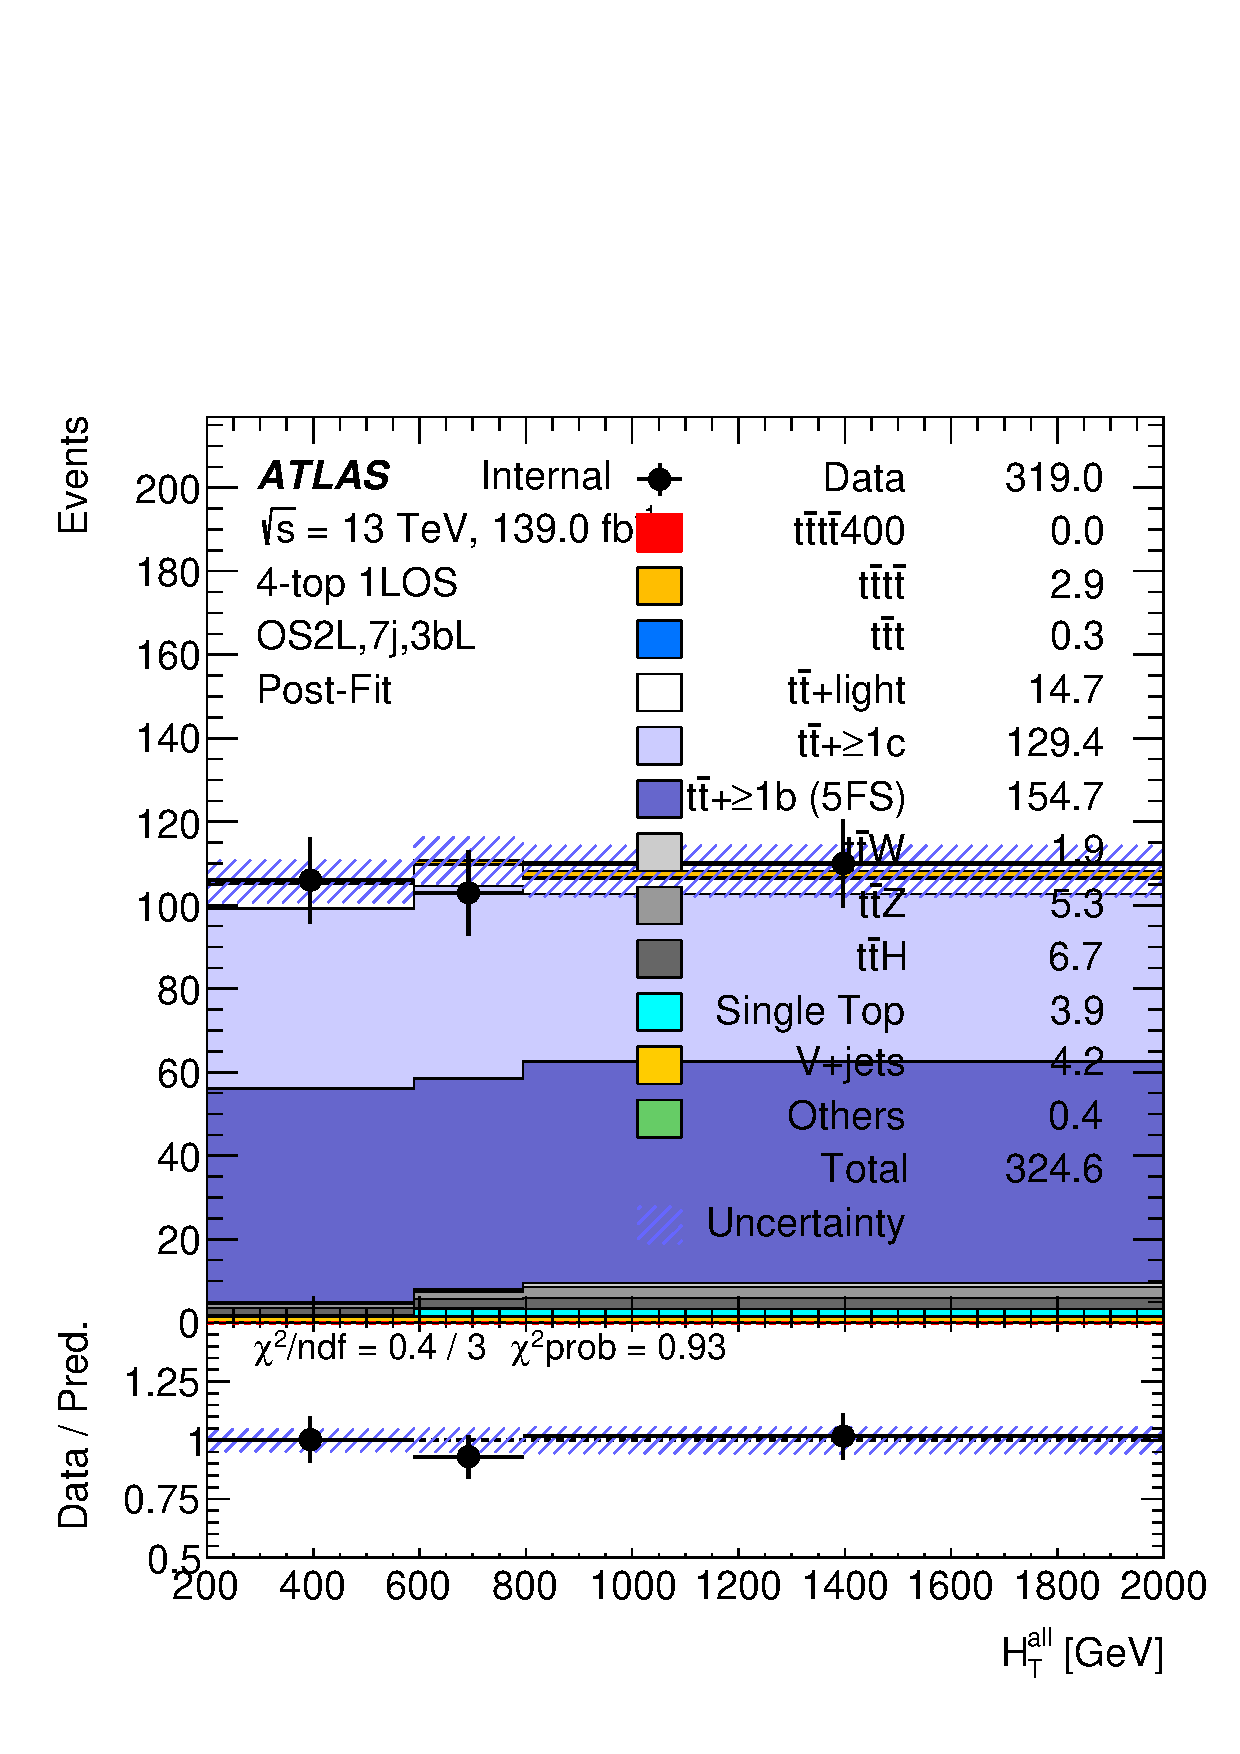
\includegraphics[width=0.31 \textwidth]{figures/fits/GNN/400/all/data_unblindedBonly/Plots/os2l_7j3bL_postFit.pdf} &
        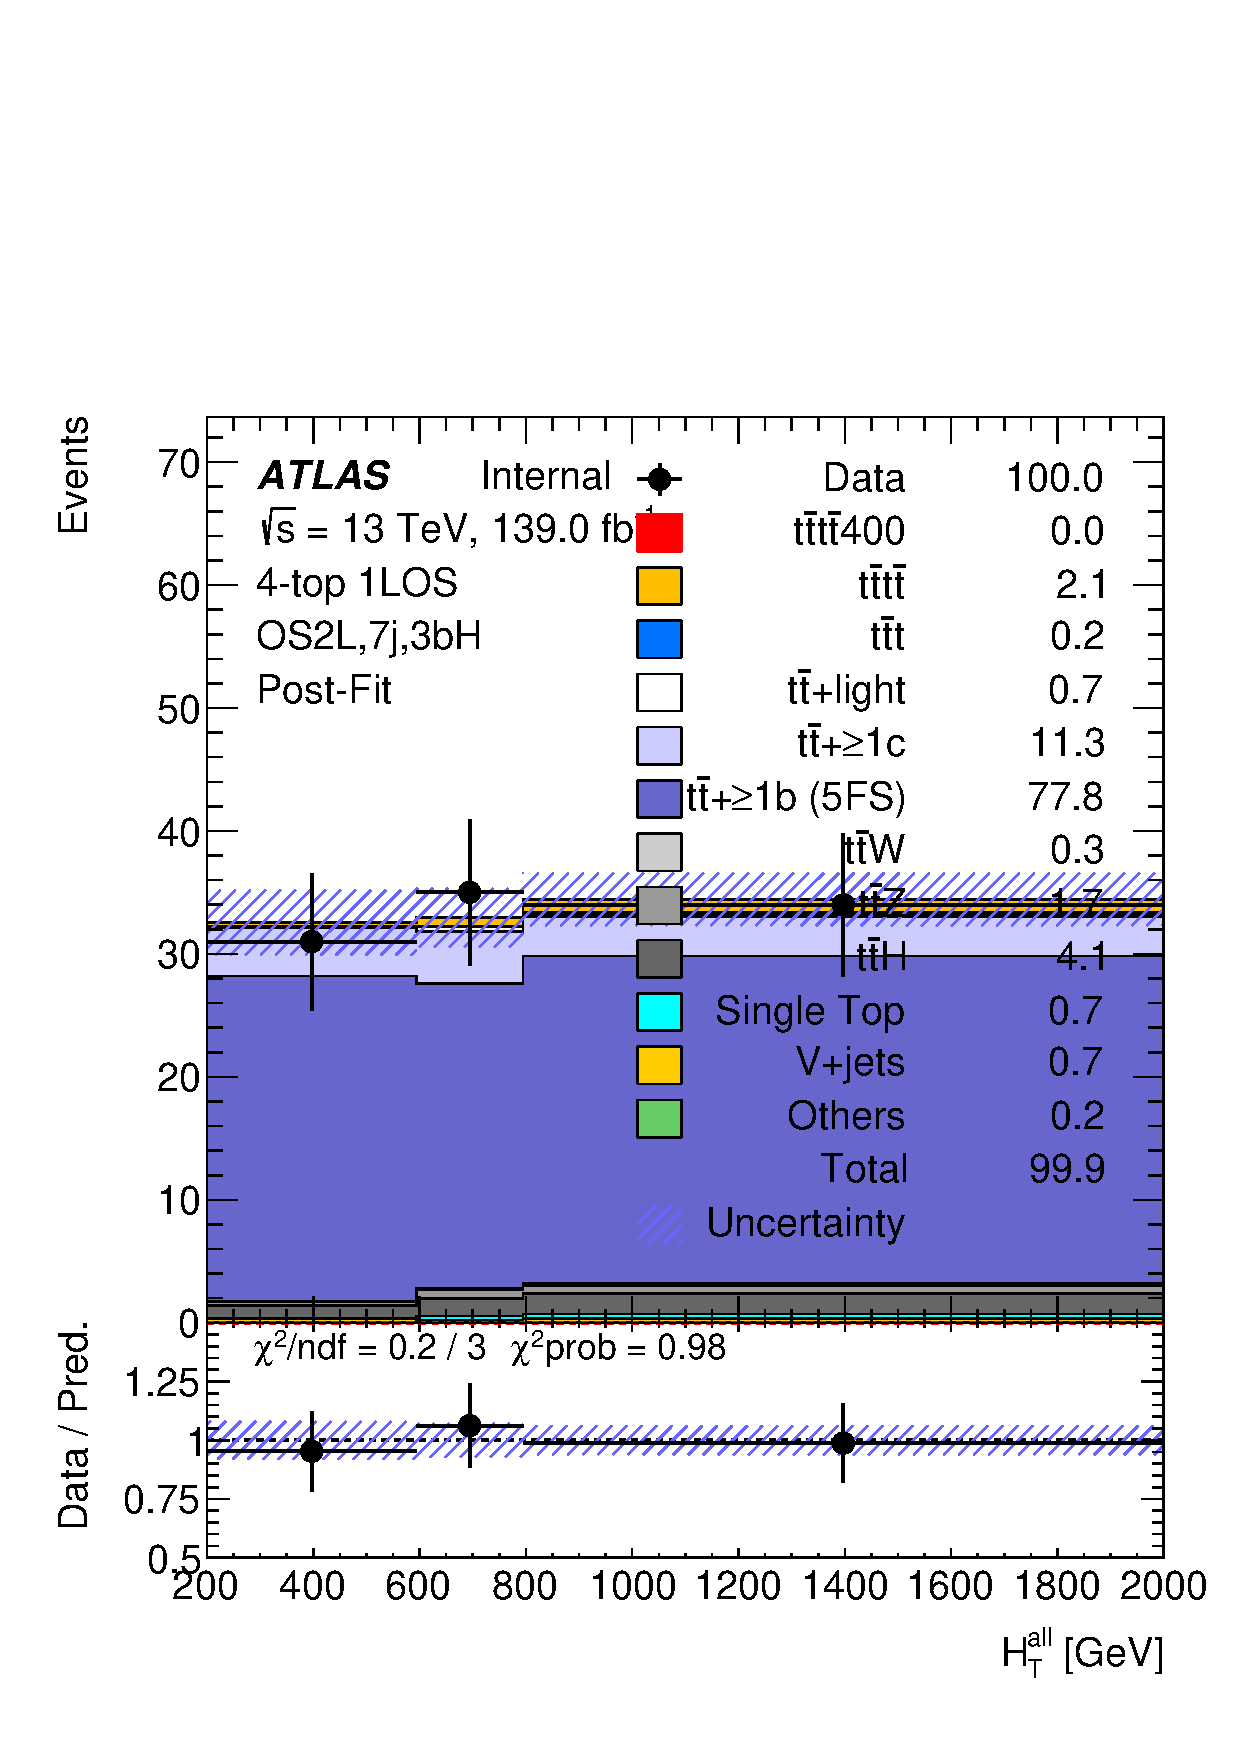
\includegraphics[width=0.31 \textwidth]{figures/fits/GNN/400/all/data_unblindedBonly/Plots/os2l_7j3bH_postFit.pdf} &
        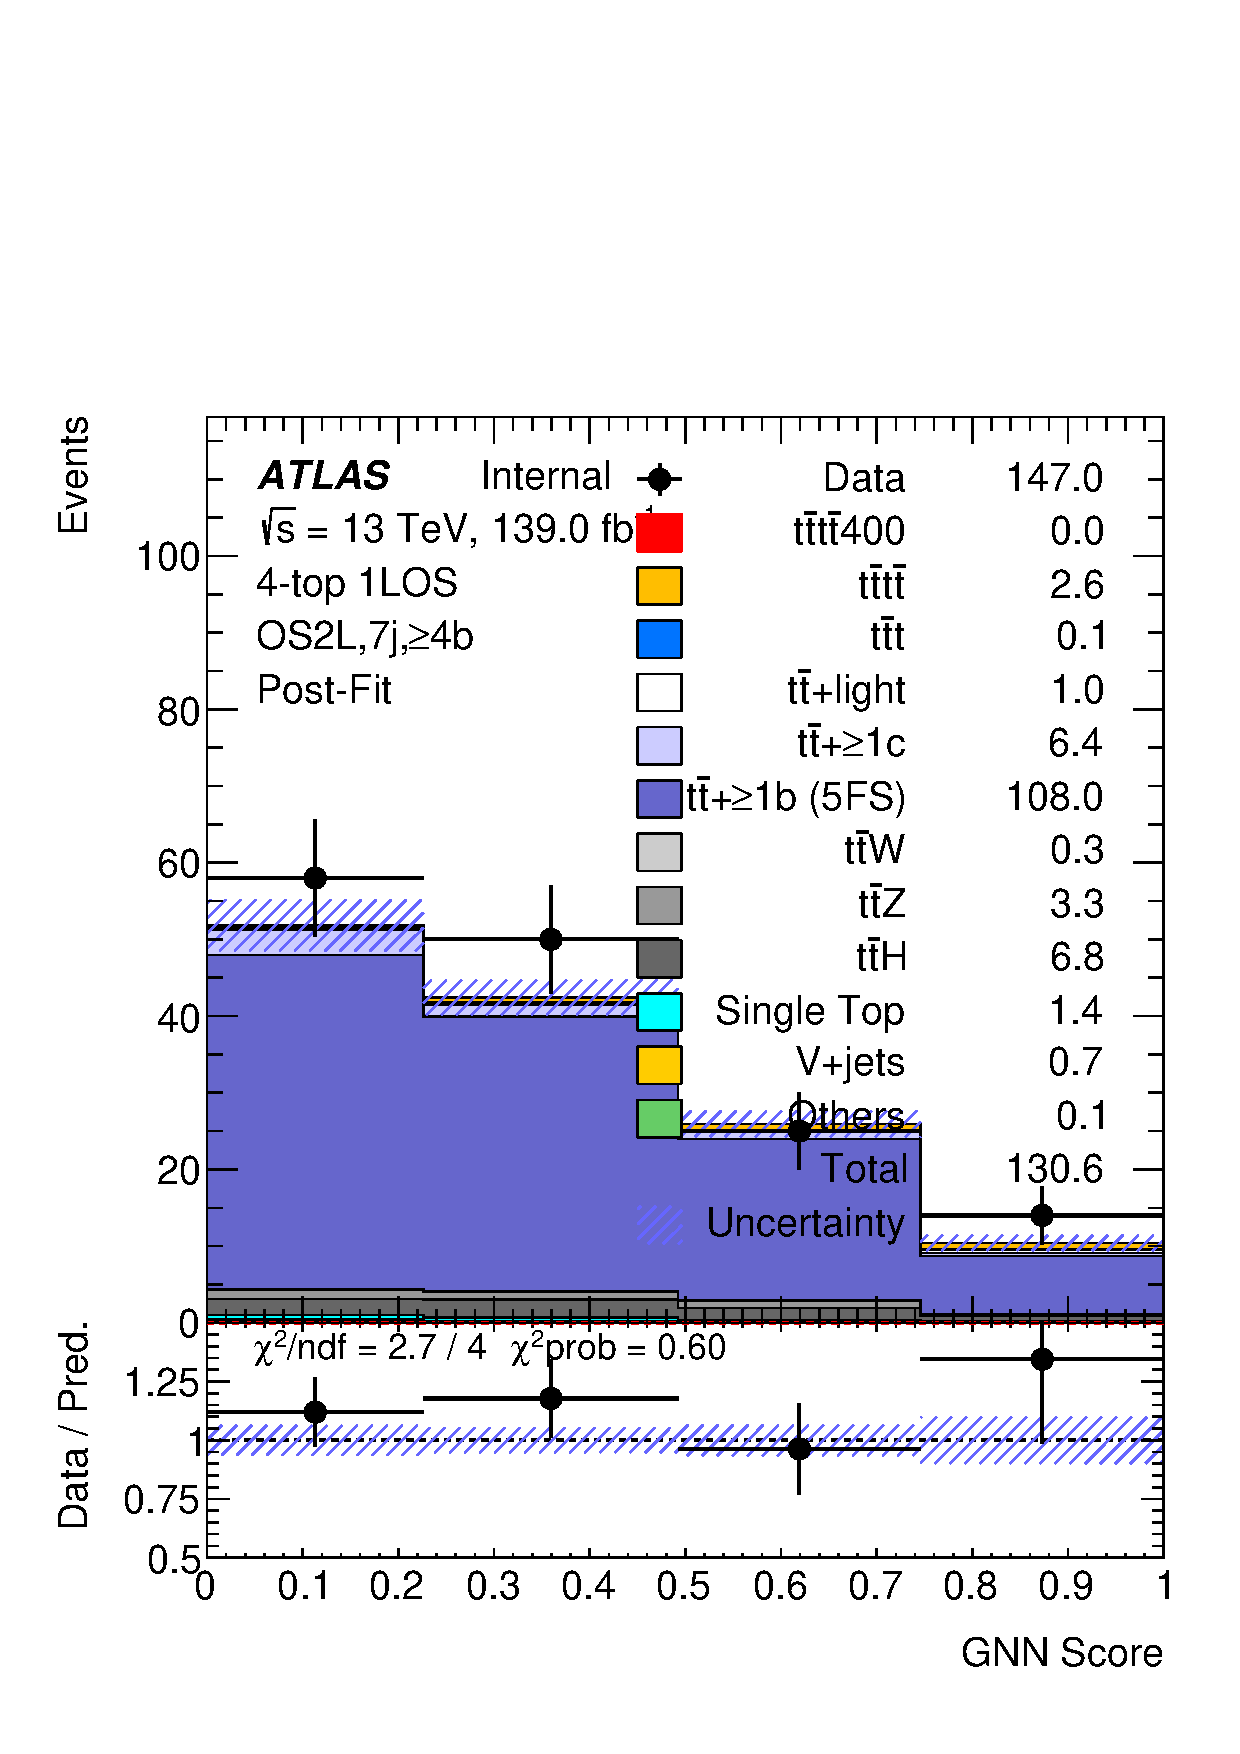
\includegraphics[width=0.31 \textwidth]{figures/fits/GNN/400/all/data_unblindedBonly/Plots/os2l_7jge4b_postFit.pdf} \\

        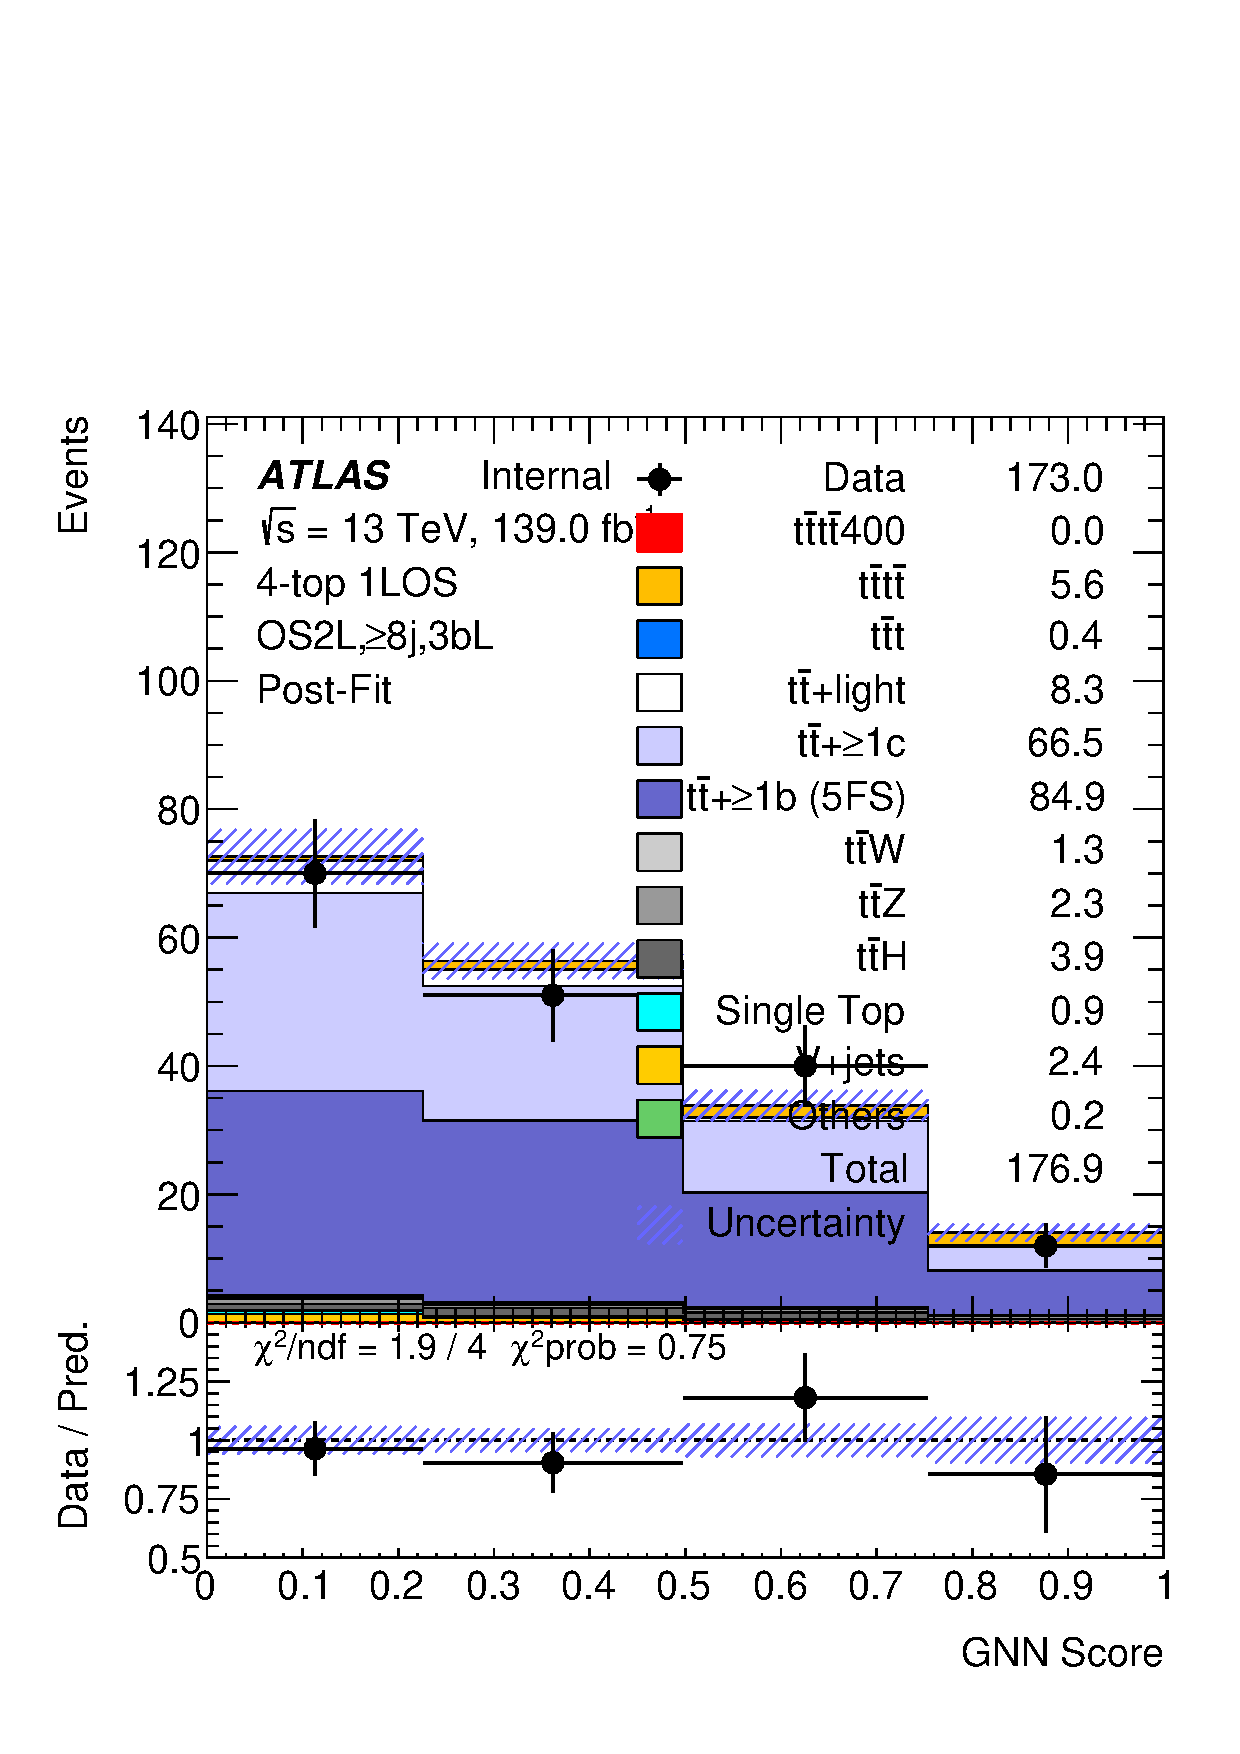
\includegraphics[width=0.31 \textwidth]{figures/fits/GNN/400/all/data_unblindedBonly/Plots/os2l_ge8j3bL_postFit.pdf} &
        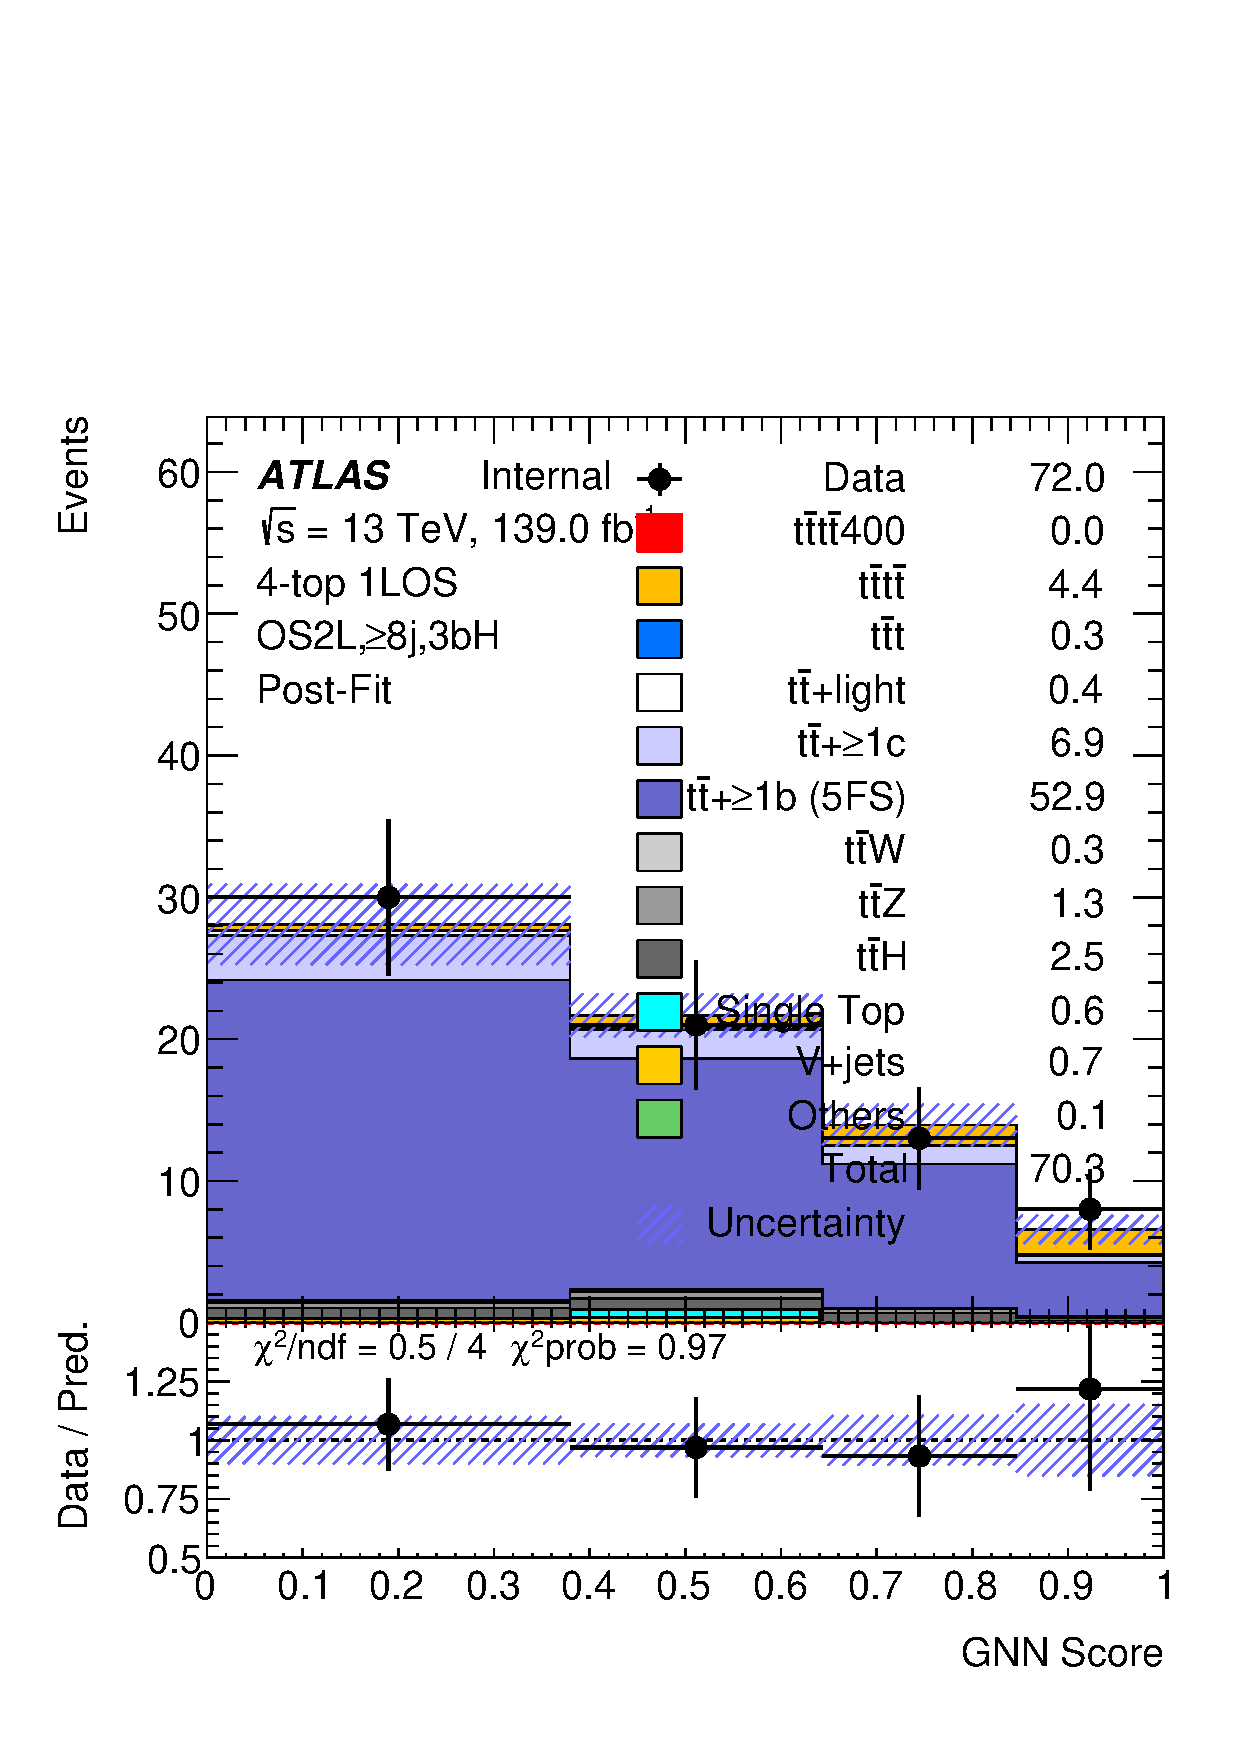
\includegraphics[width=0.31 \textwidth]{figures/fits/GNN/400/all/data_unblindedBonly/Plots/os2l_ge8j3bH_postFit.pdf} &
        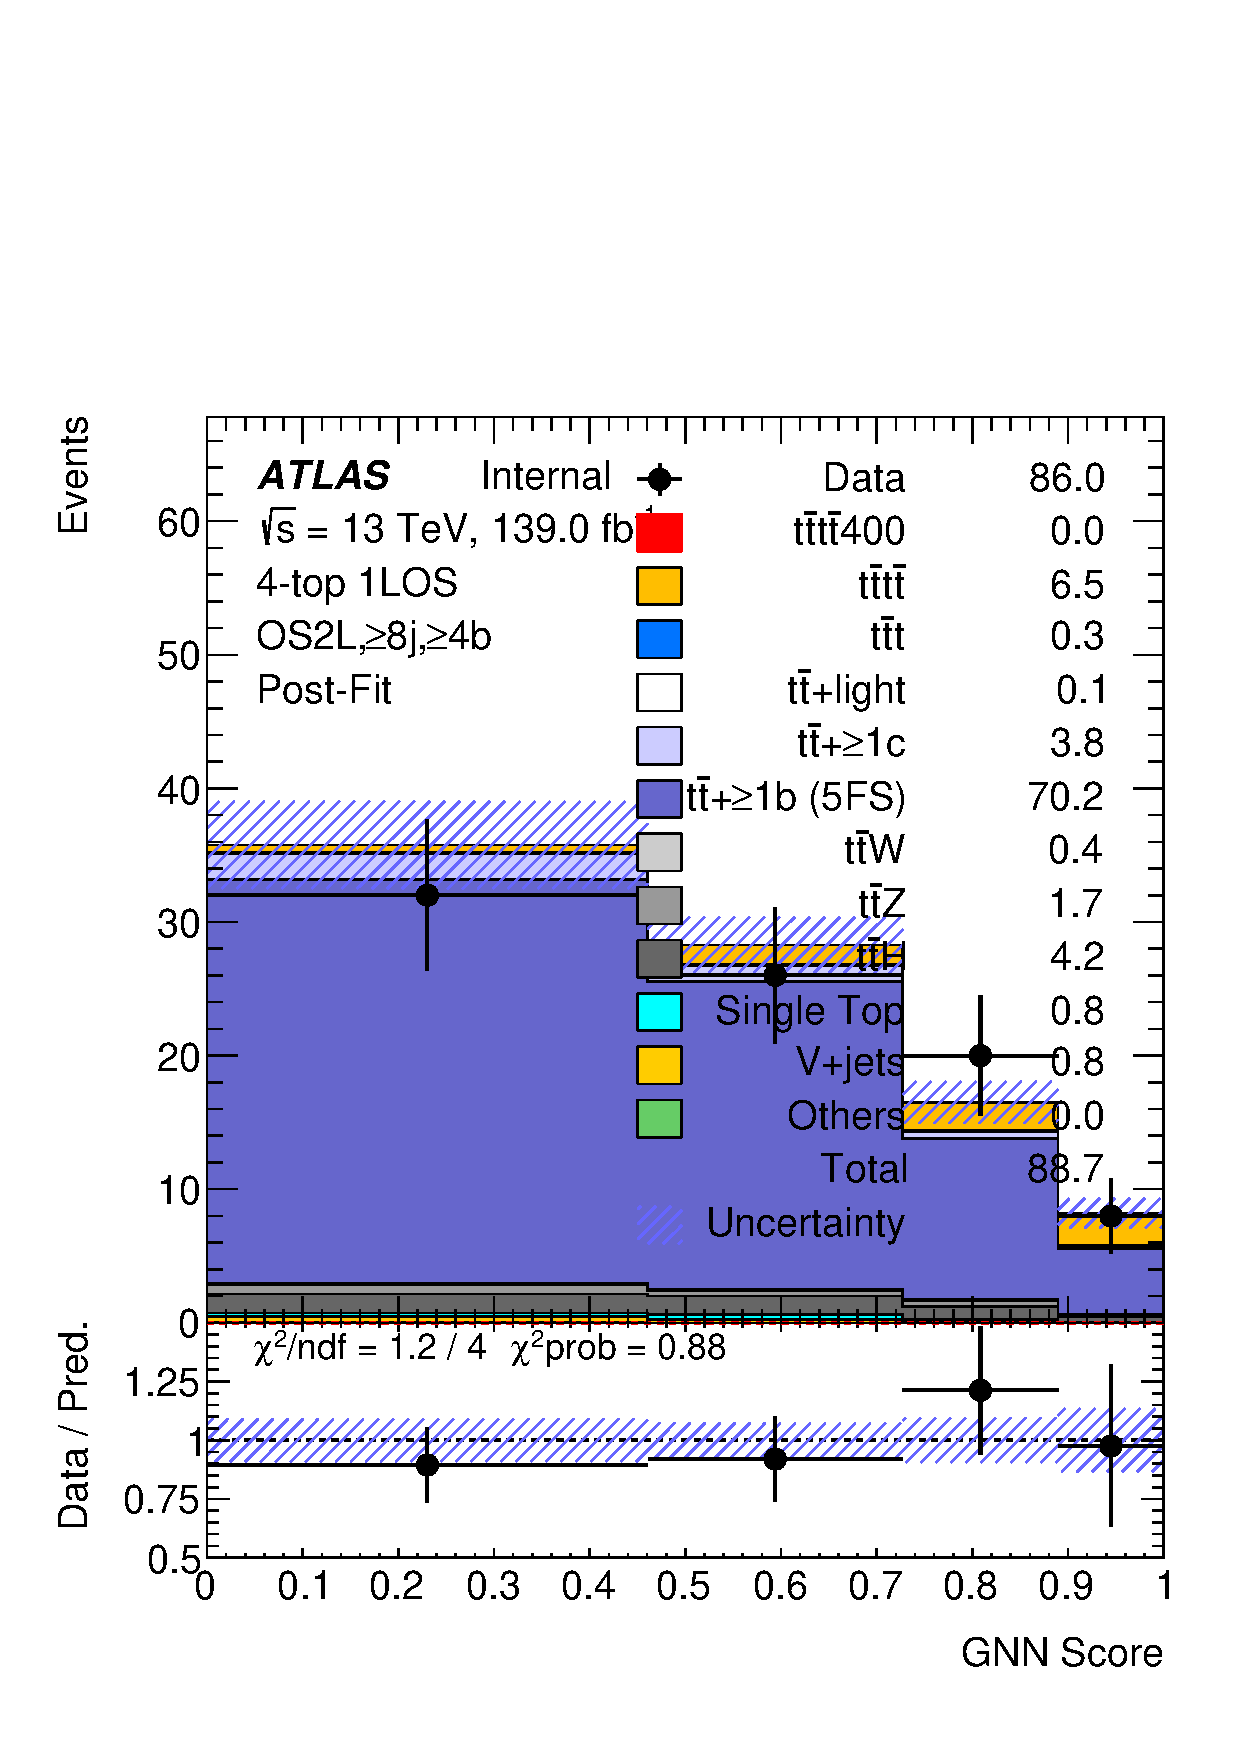
\includegraphics[width=0.31 \textwidth]{figures/fits/GNN/400/all/data_unblindedBonly/Plots/os2l_ge8jge4b_postFit.pdf} \\
        \end{tabular}
        \caption{\label{fig:unblinded_data_Bonly_postfit_2L}Post-fit distributions for 2LOS regions obtained with background-only unblinded data fit, compared with data yields for mH = 400 GeV. The fit is done using all regions (1L+2L)}
\end{center}
\end{figure}


\begin{figure}[htbp!]
  \centering
  \begin{subfigure}[t]{0.32\textwidth}
    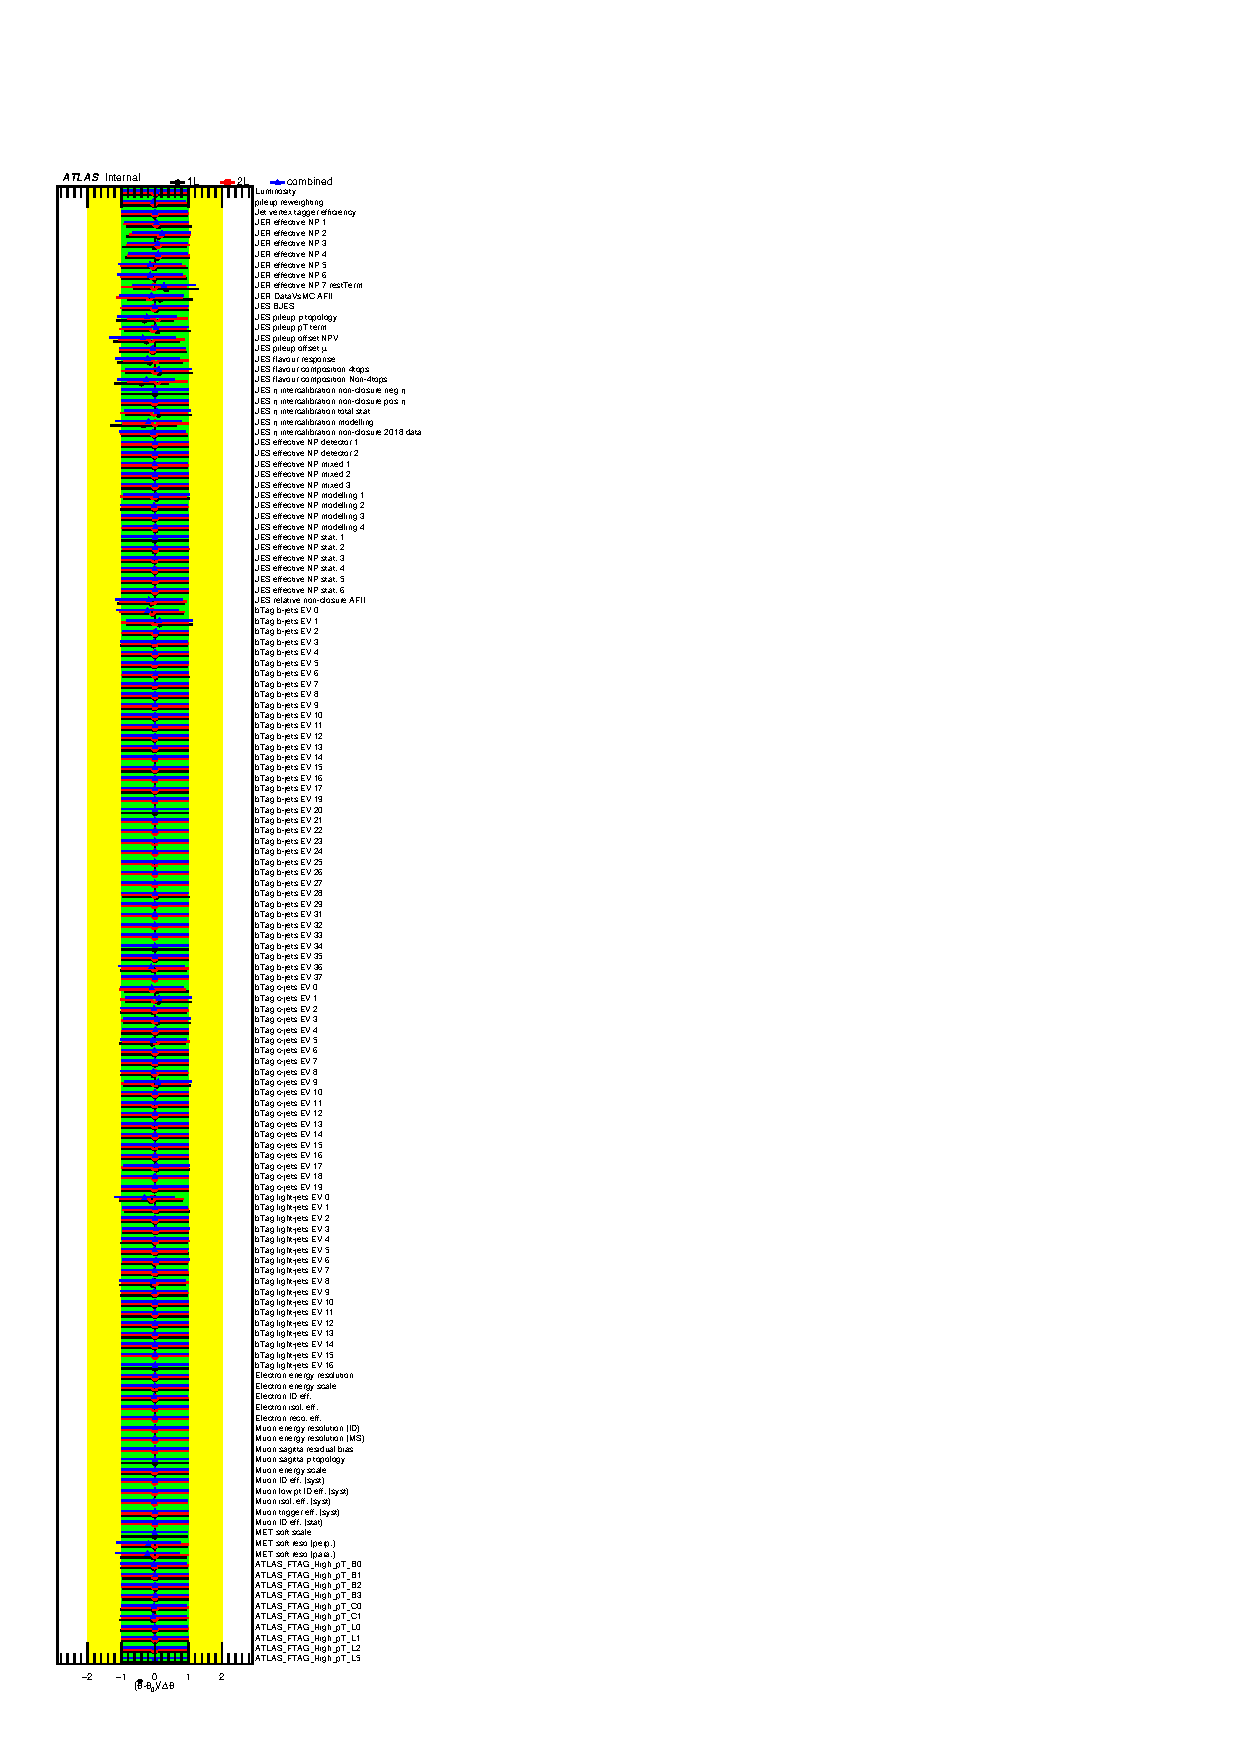
\includegraphics[width=\linewidth]{figures/fits/comparisons/selections/GNN/400/data_unblindedBonly/NuisPar_comp_Instrumental.pdf}
    \subcaption{mH=400\gev}
    \label{fig:unblinded_data_Bonly_NP_mH400}
  \end{subfigure}
  \begin{subfigure}[t]{0.32\textwidth}
    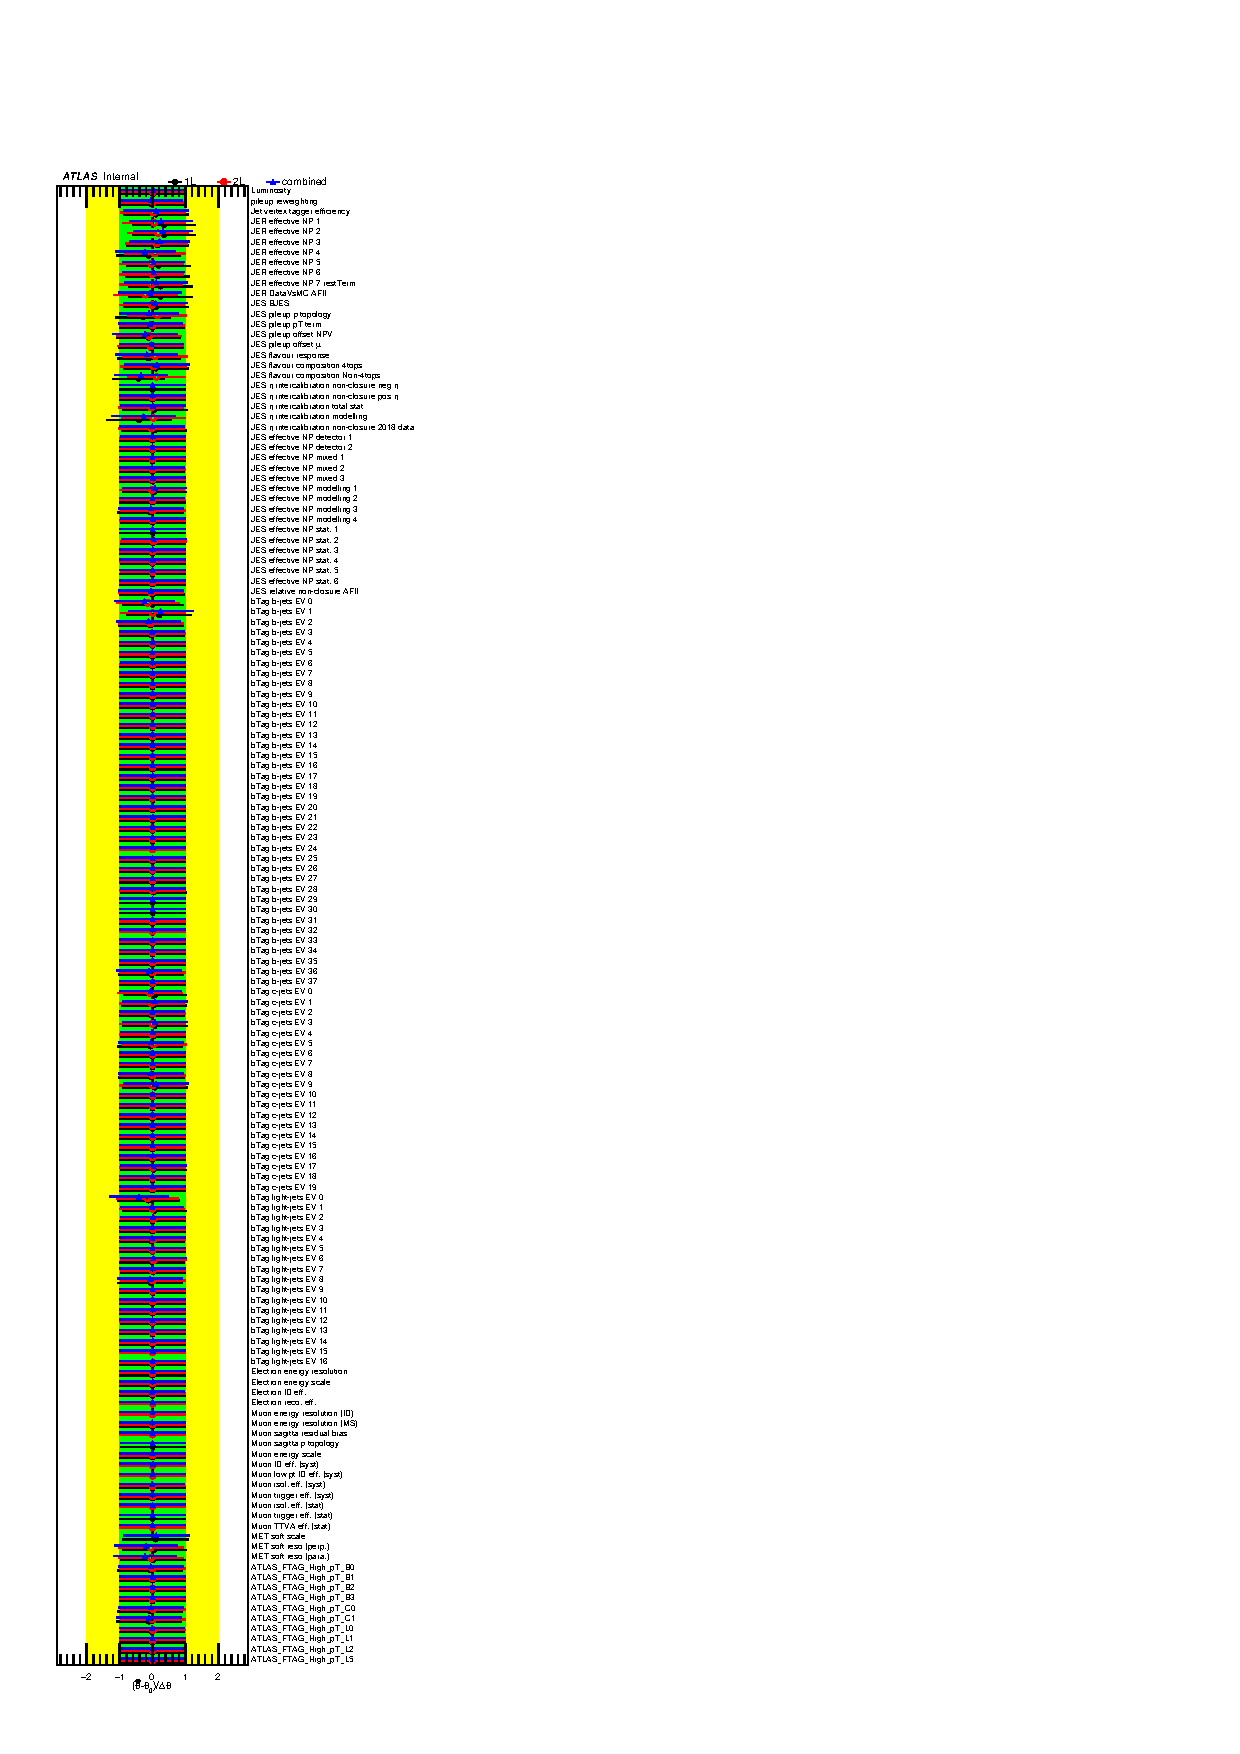
\includegraphics[width=\linewidth]{figures/fits/comparisons/selections/GNN/700/data_unblindedBonly/NuisPar_comp_Instrumental.pdf}
    \subcaption{mH=700\gev}
    \label{fig:unblinded_data_Bonly_NP_mH400}
  \end{subfigure}
  \begin{subfigure}[t]{0.32\textwidth}
    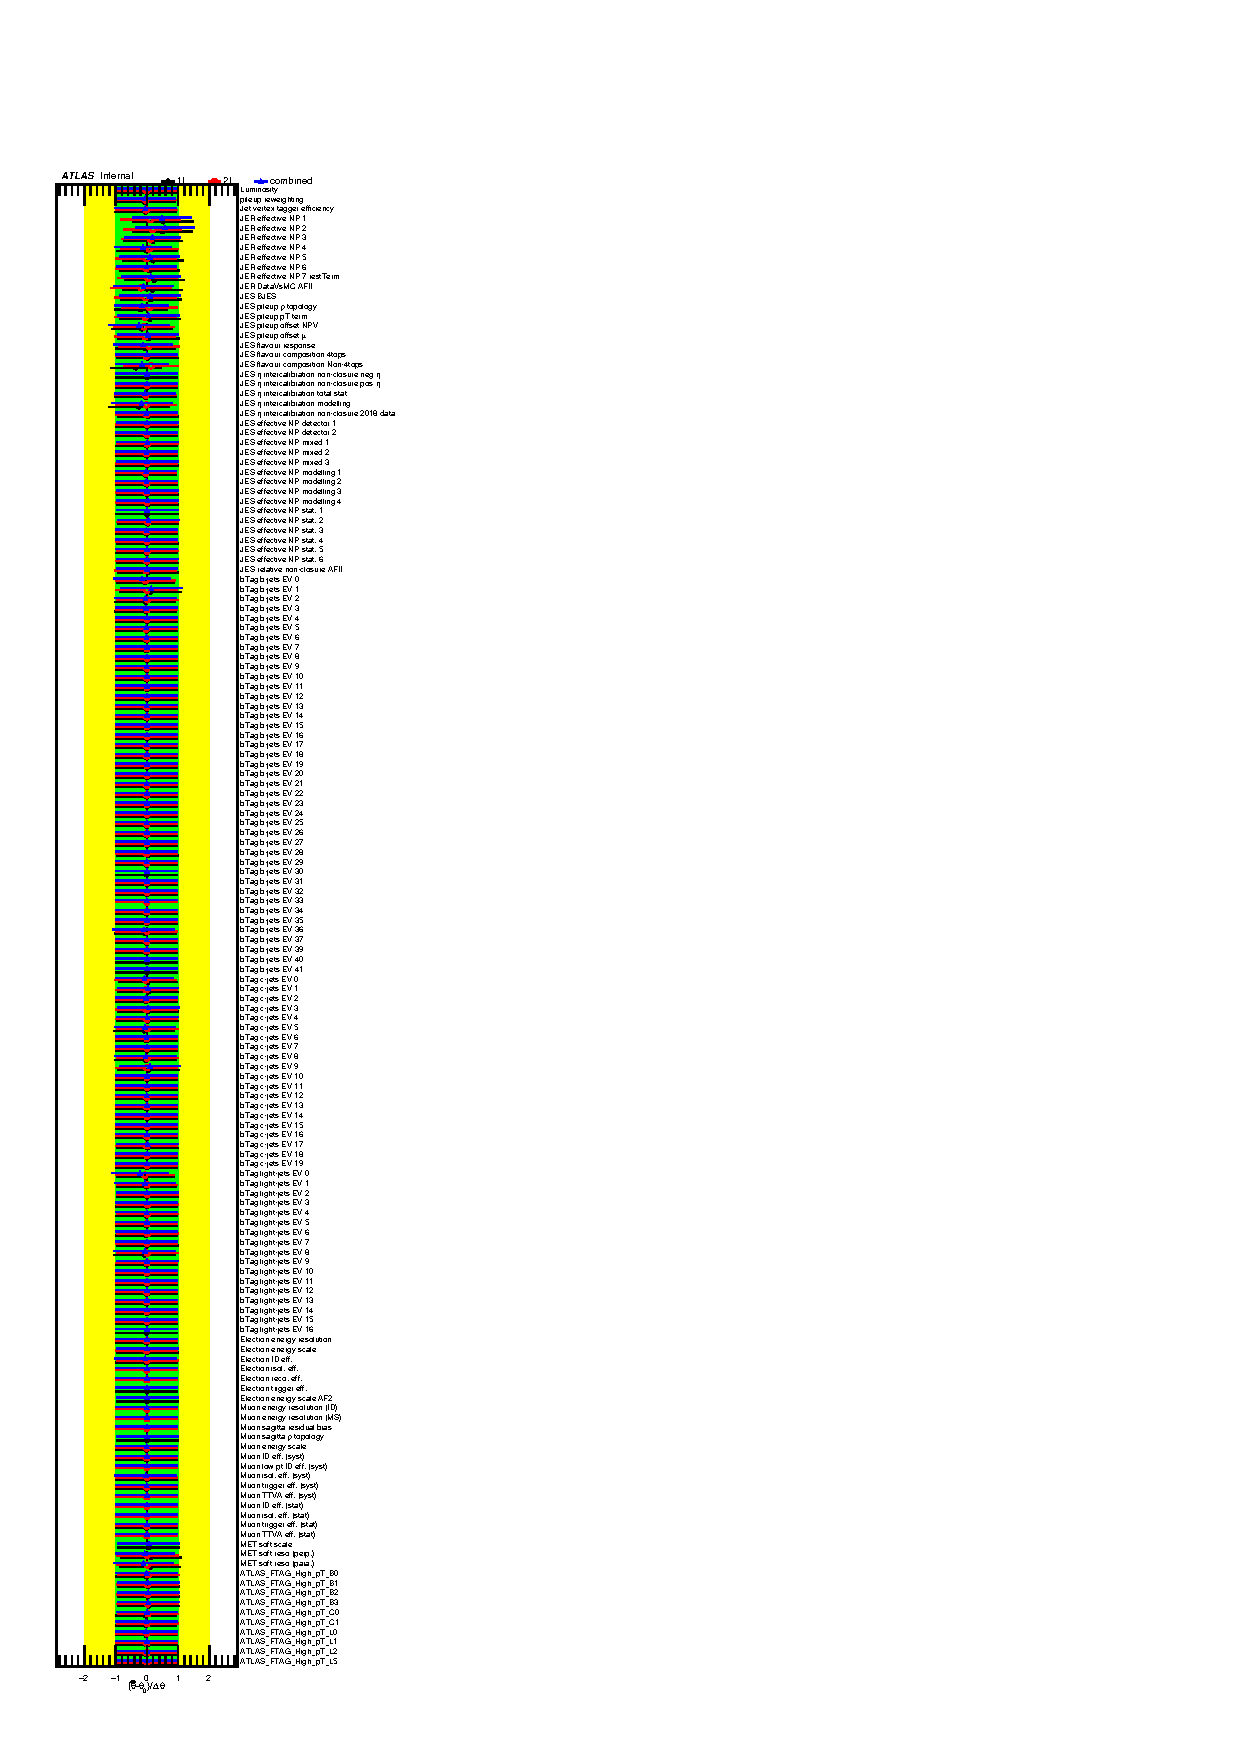
\includegraphics[width=\linewidth]{figures/fits/comparisons/selections/GNN/1000/data_unblindedBonly/NuisPar_comp_Instrumental.pdf}
    \subcaption{mH=1000\gev}
    \label{fig:unblinded_data_Bonly_NP_mH400}
  \end{subfigure}
  \caption{\label{fig:unblinded_data_Bonly_NP_instrumental}Fitted pulls and constraints for the nuisance parameters corresponding to the instrumental systematic uncertainties for the background-only unblinded Data fit for three mass points. Comparison is done for three fits: using only 1L regions, using only 2LOS regions and using all regions.}
\end{figure}


\begin{figure}[htbp!]
  \centering
  \begin{subfigure}[t]{0.32\textwidth}
    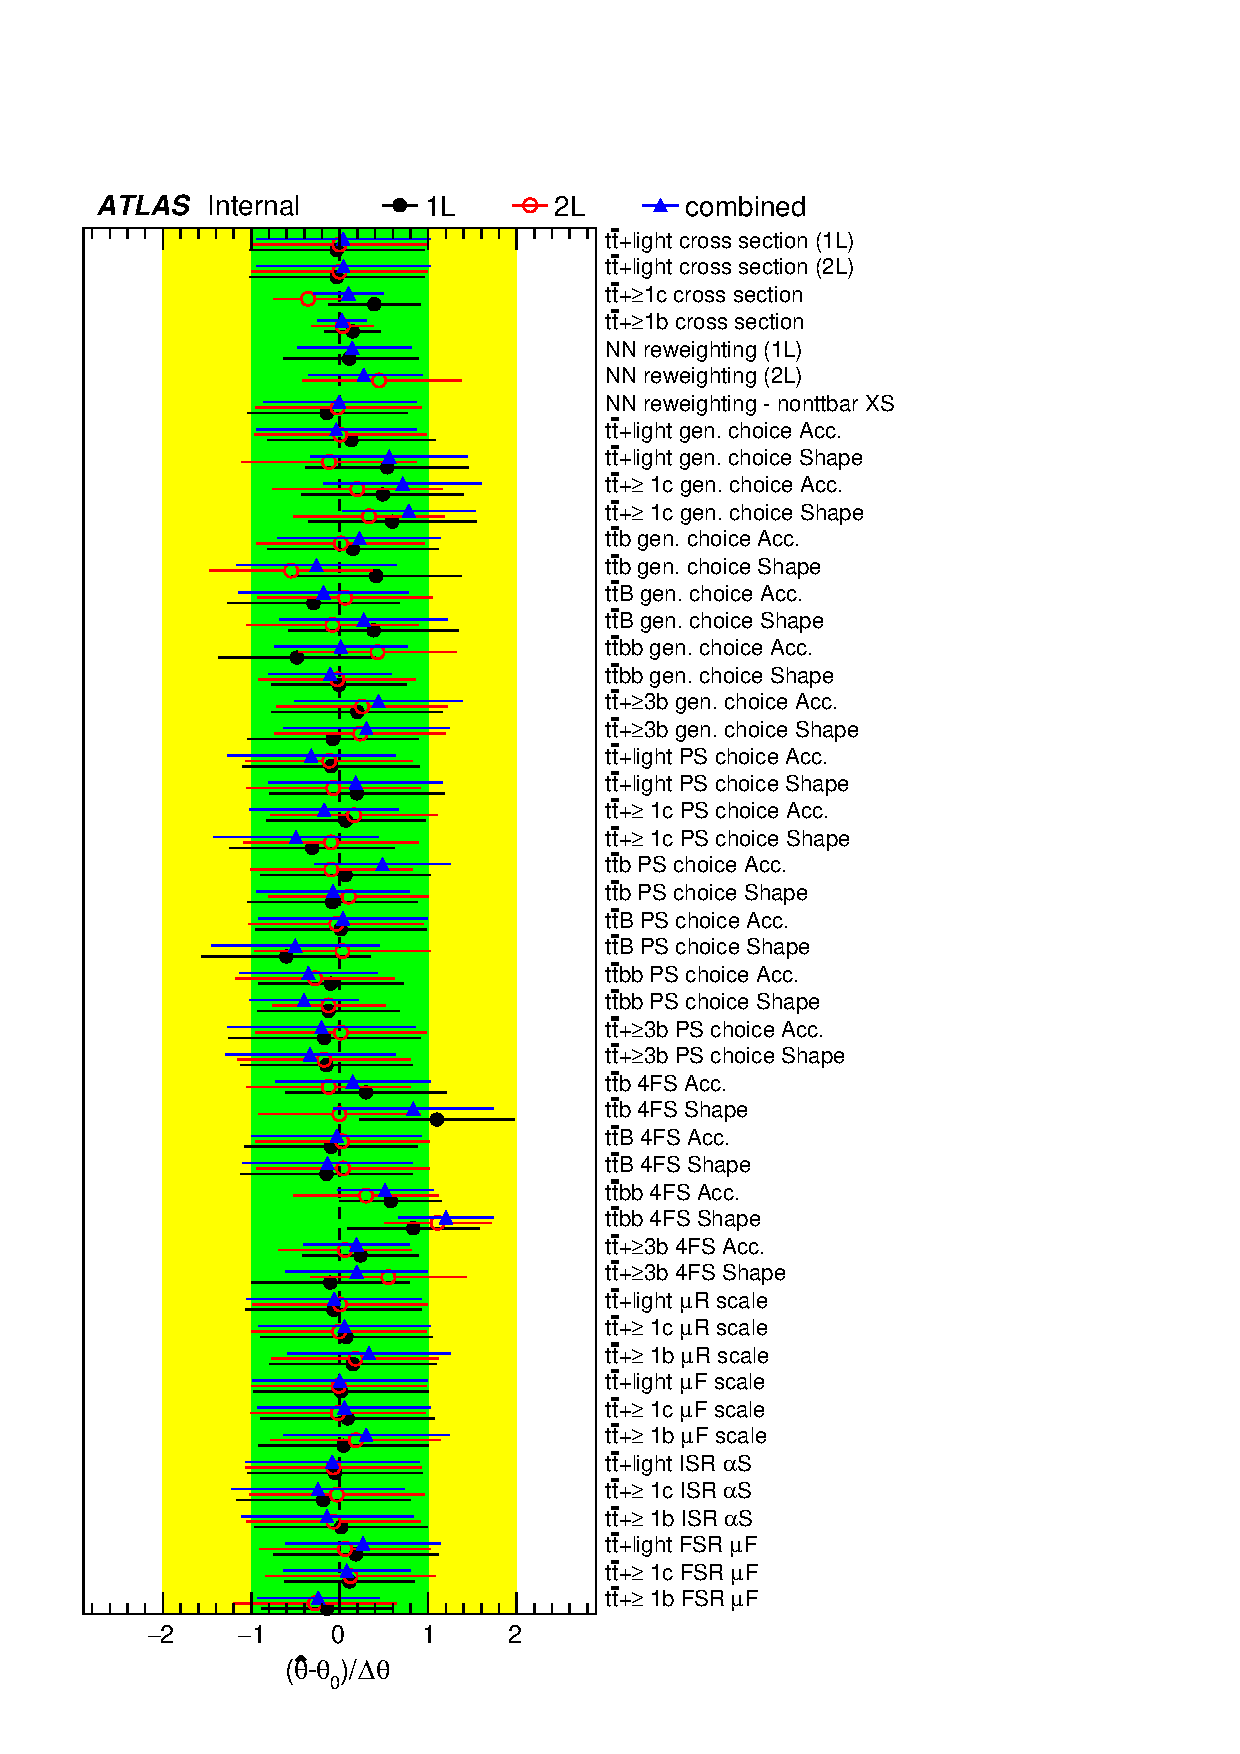
\includegraphics[width=\linewidth]{figures/fits/comparisons/selections/GNN/400/data_unblindedBonly/NuisPar_comp_ttbar.pdf}
    \subcaption{mH=400\gev}
    \label{fig:unblinded_data_Bonly_NP_mH400}
  \end{subfigure}
  \begin{subfigure}[t]{0.32\textwidth}
    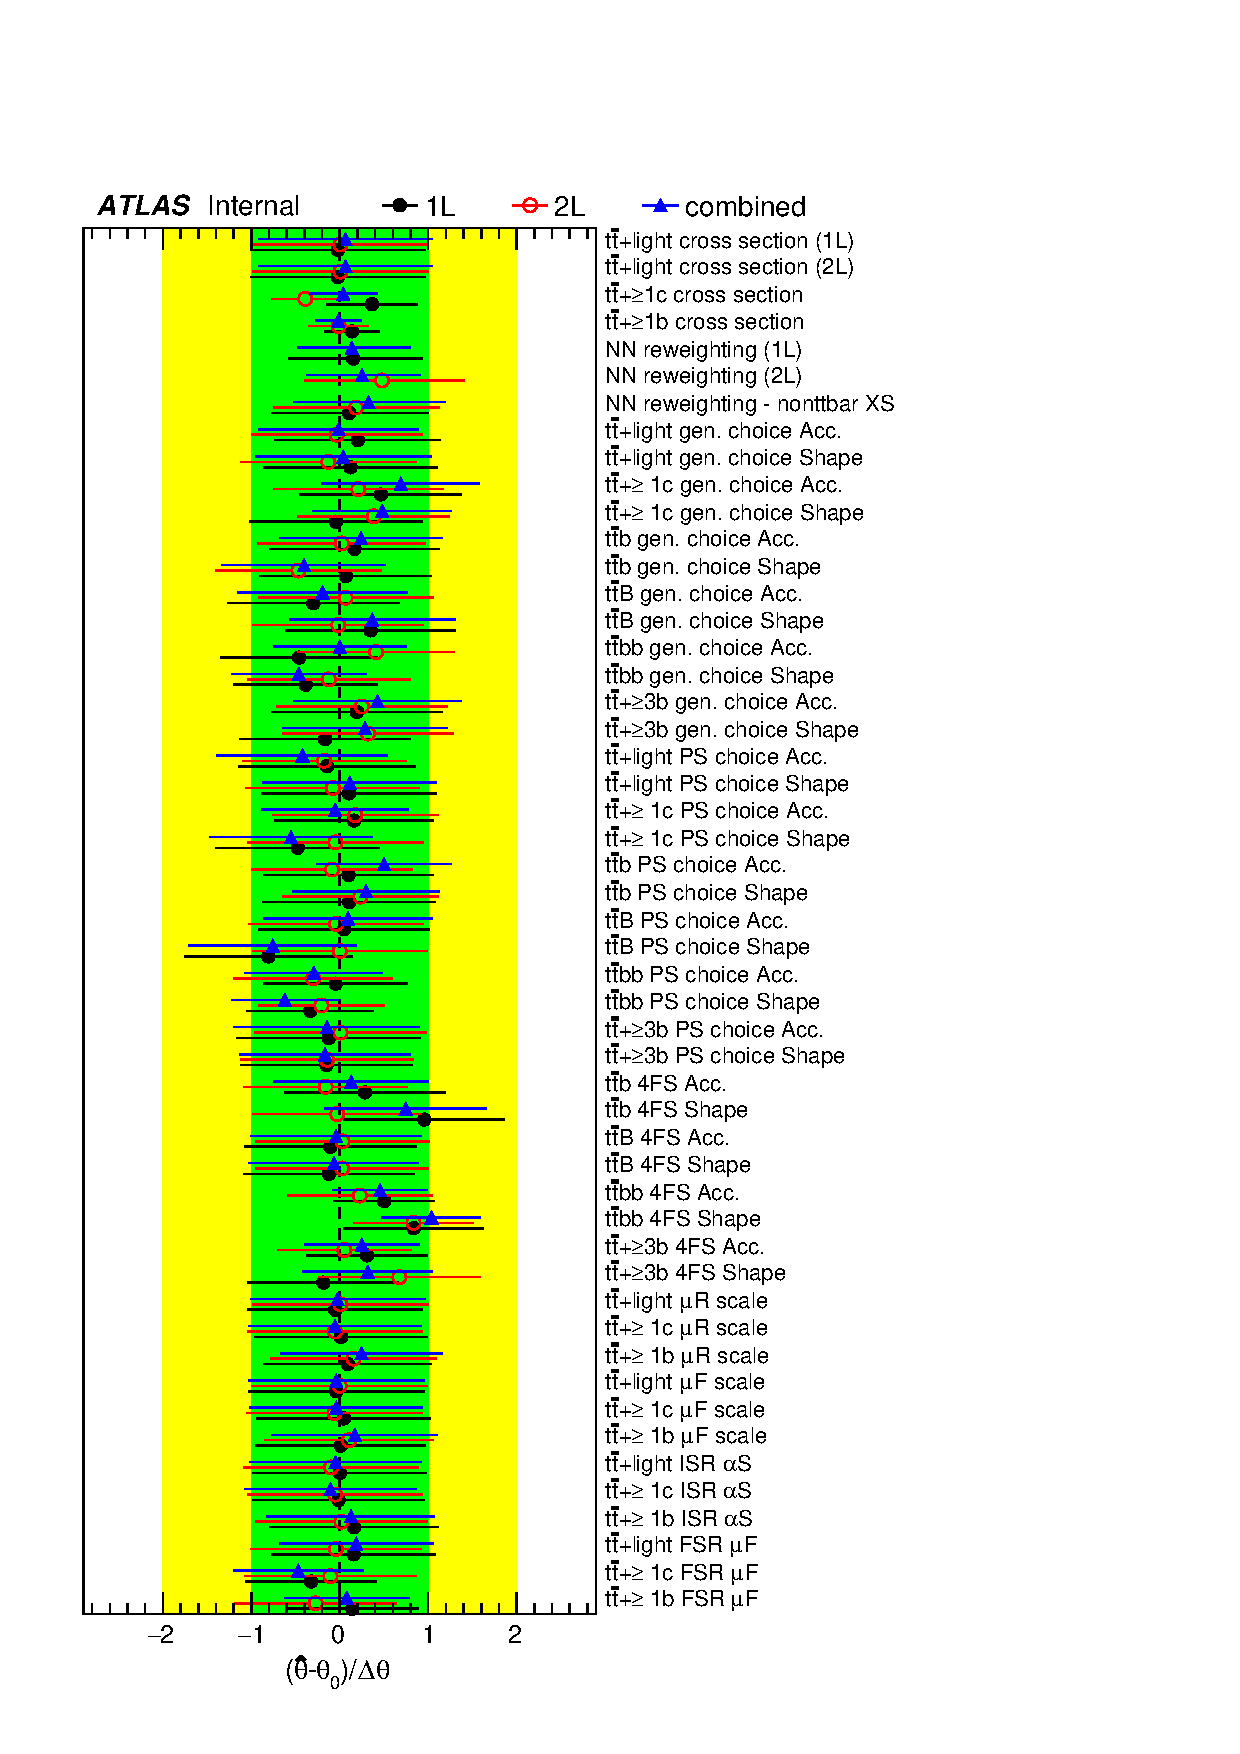
\includegraphics[width=\linewidth]{figures/fits/comparisons/selections/GNN/700/data_unblindedBonly/NuisPar_comp_ttbar.pdf}
    \subcaption{mH=700\gev}
    \label{fig:unblinded_data_Bonly_NP_mH400}
  \end{subfigure}
  \begin{subfigure}[t]{0.32\textwidth}
    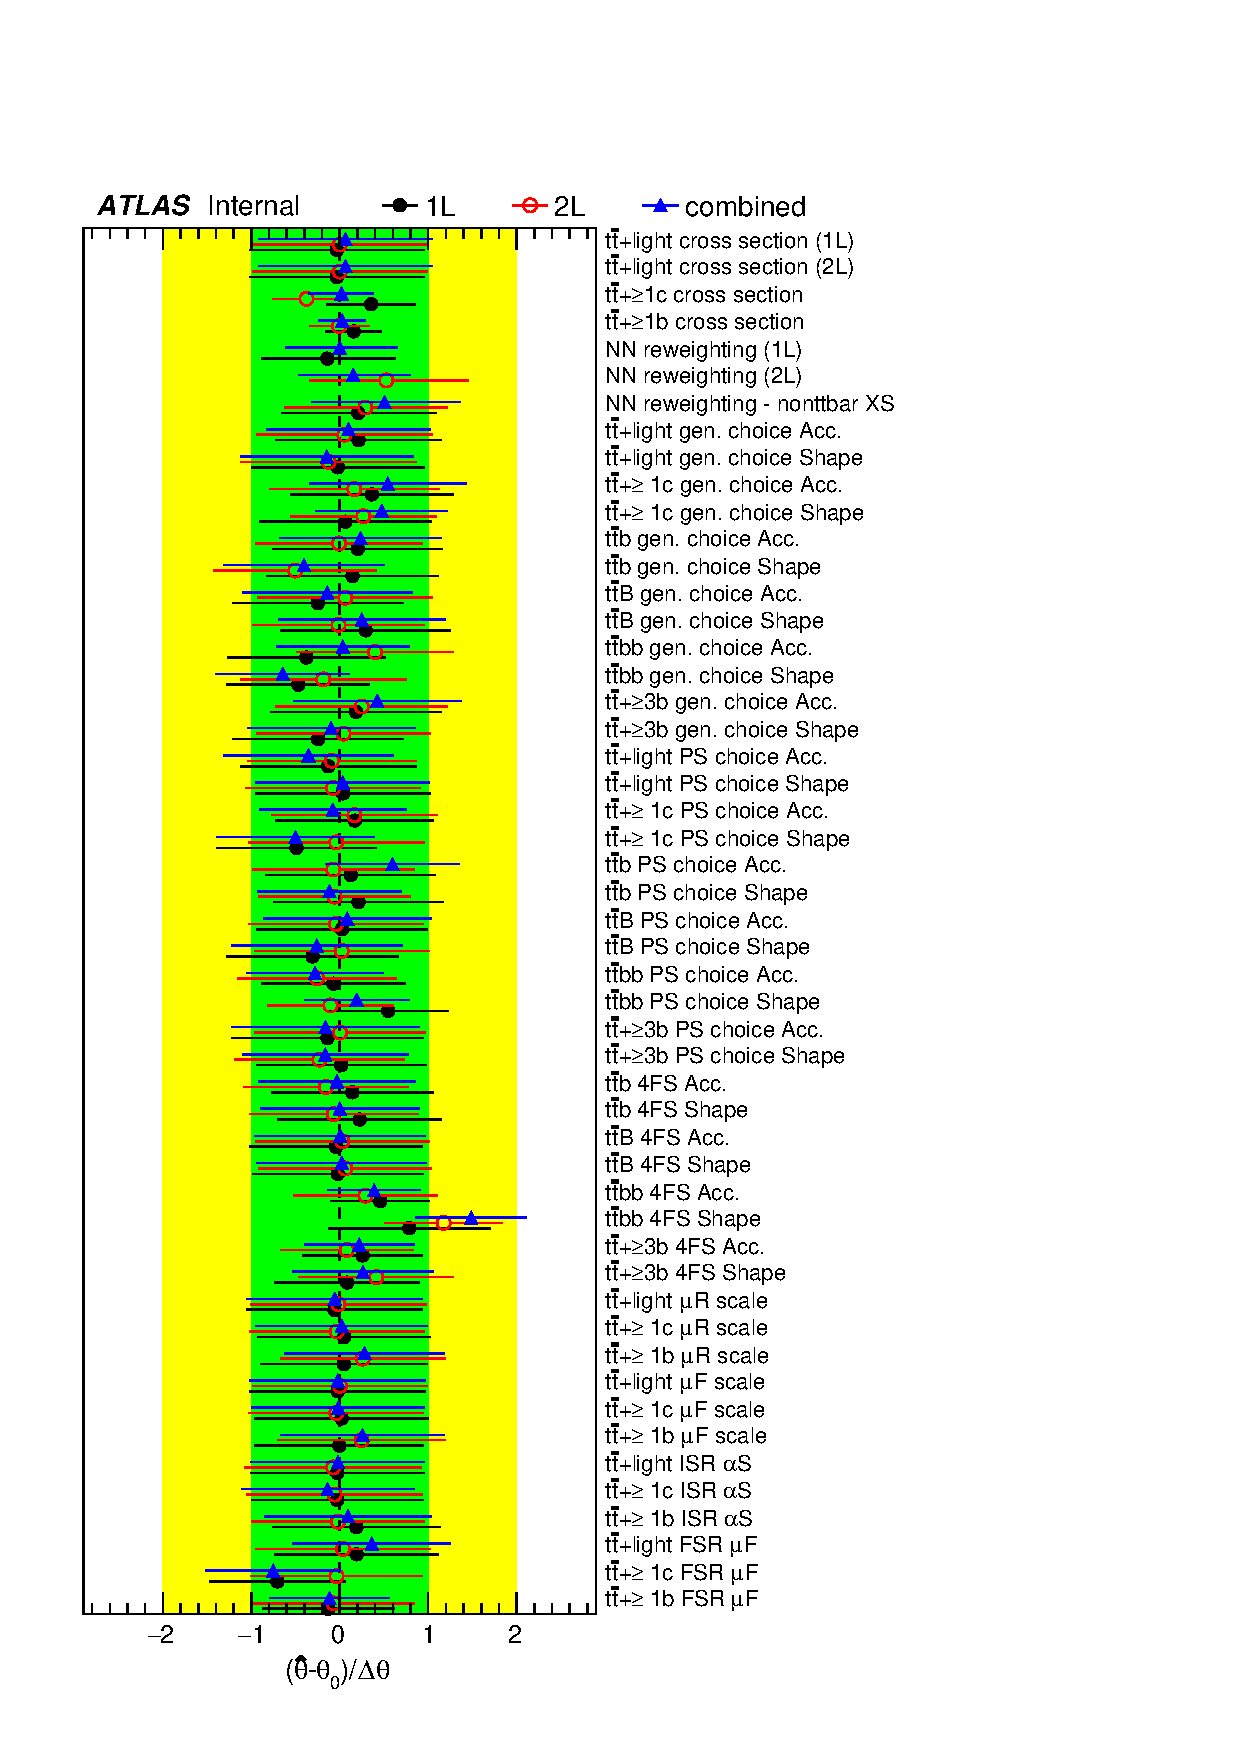
\includegraphics[width=\linewidth]{figures/fits/comparisons/selections/GNN/1000/data_unblindedBonly/NuisPar_comp_ttbar.pdf}
    \subcaption{mH=1000\gev}
    \label{fig:unblinded_data_Bonly_NP_mH400}
  \end{subfigure}
  \caption{\label{fig:unblinded_data_Bonly_NP_ttbar}Fitted pulls and constraints for the nuisance parameters corresponding to the \ttbar systematic uncertainties for the background-only unblinded Data fit for three mass points. Comparison is done for three fits: using only 1L regions, using only 2LOS regions and using all regions.}
\end{figure}


\begin{figure}[htbp!]
  \centering
  \begin{subfigure}[t]{0.32\textwidth}
    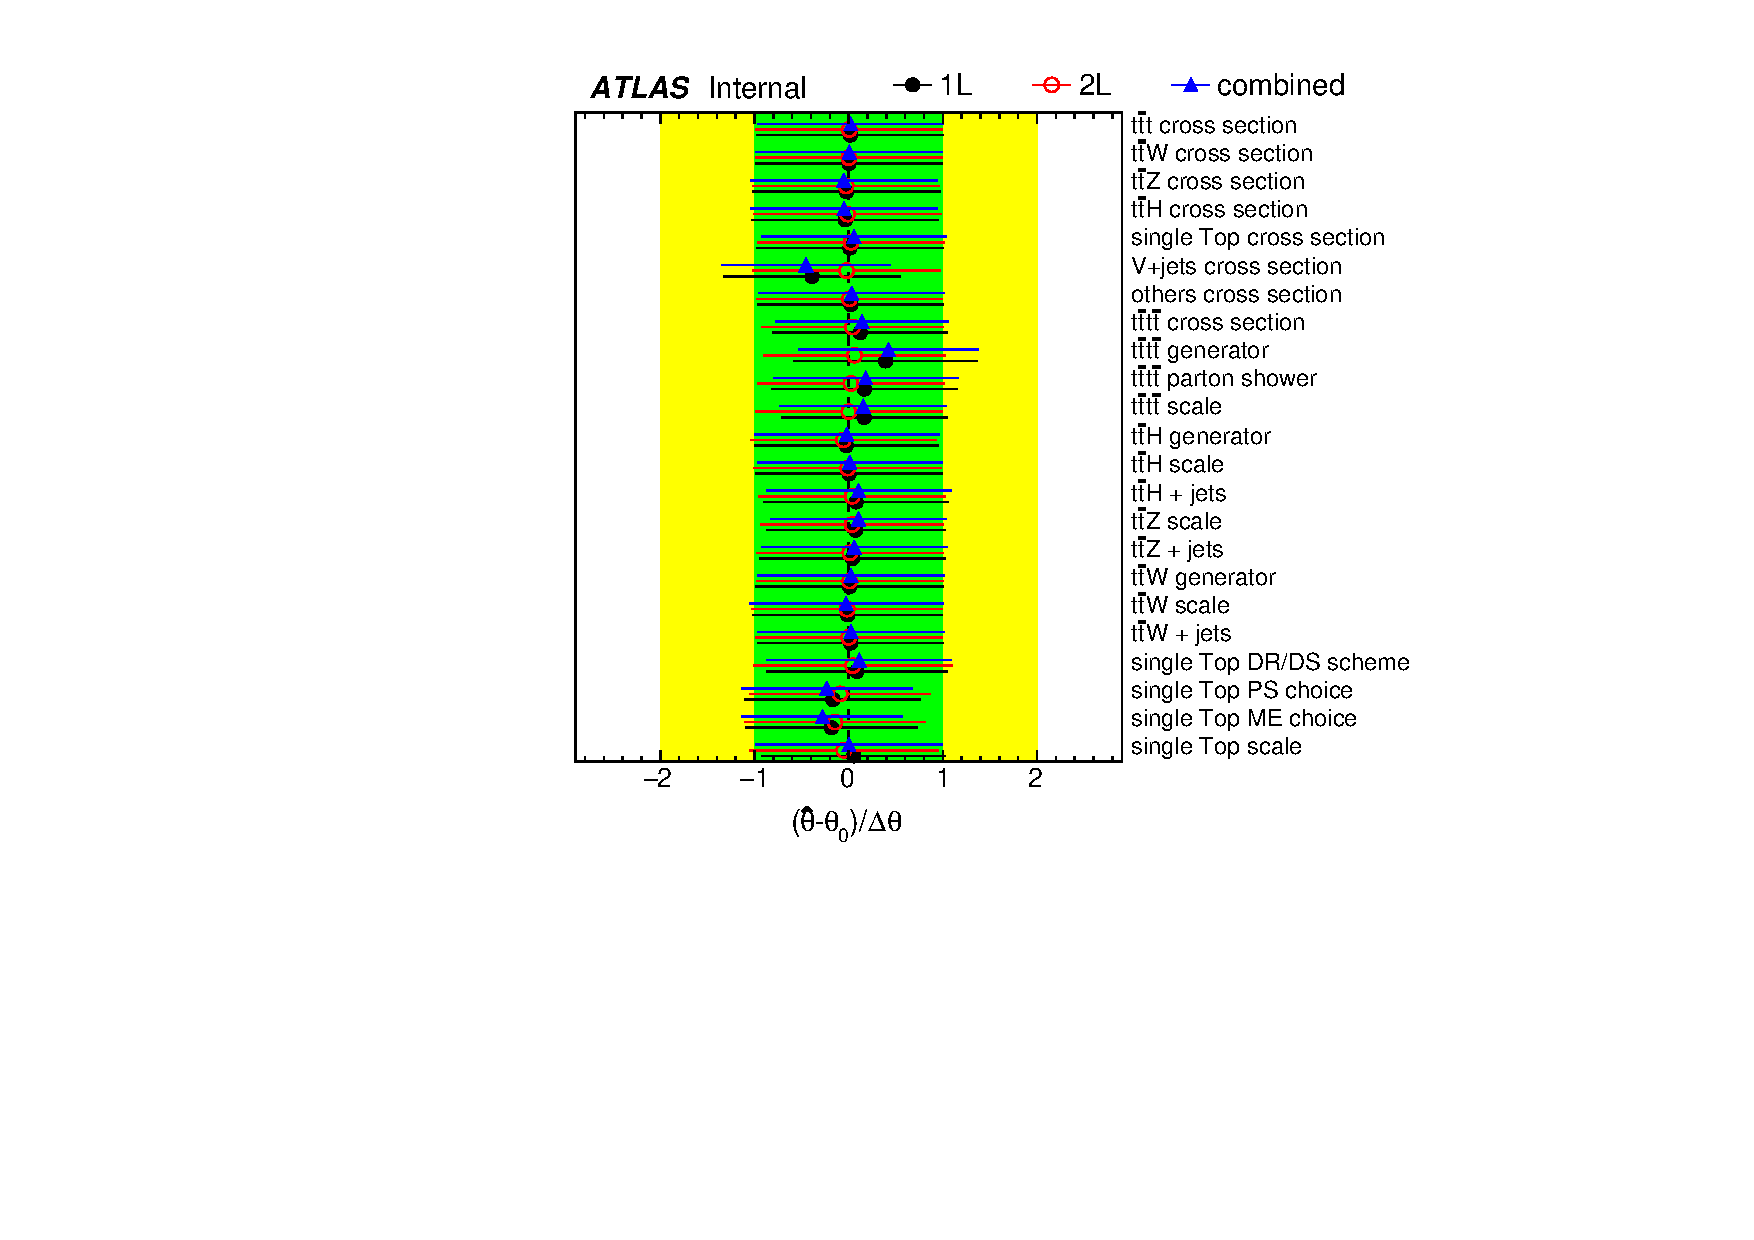
\includegraphics[width=\linewidth]{figures/fits/comparisons/selections/GNN/400/data_unblindedBonly/NuisPar_comp_Other.pdf}
    \subcaption{mH=400\gev}
    \label{fig:unblinded_data_Bonly_NP_mH400}
  \end{subfigure}
  \begin{subfigure}[t]{0.32\textwidth}
    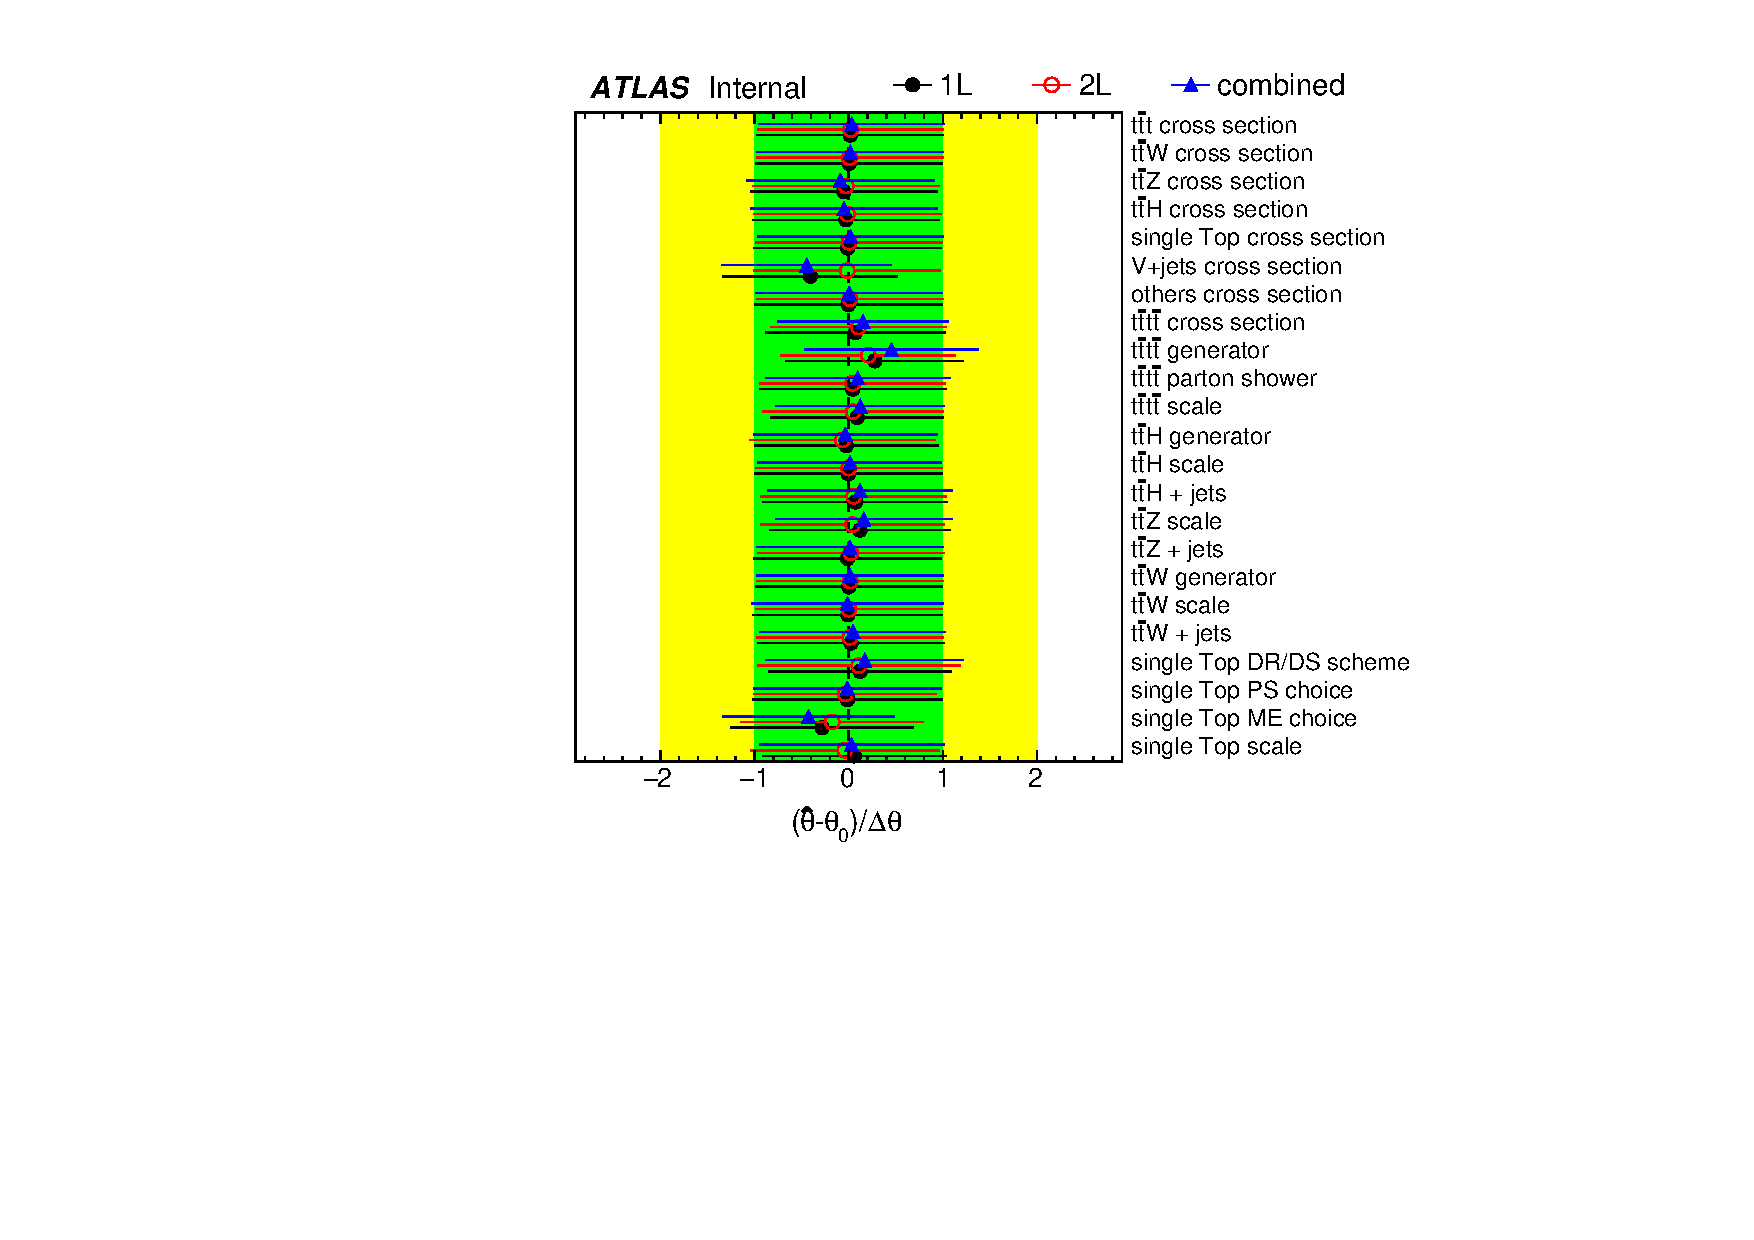
\includegraphics[width=\linewidth]{figures/fits/comparisons/selections/GNN/700/data_unblindedBonly/NuisPar_comp_Other.pdf}
    \subcaption{mH=700\gev}
    \label{fig:unblinded_data_Bonly_NP_mH400}
  \end{subfigure}
  \begin{subfigure}[t]{0.32\textwidth}
    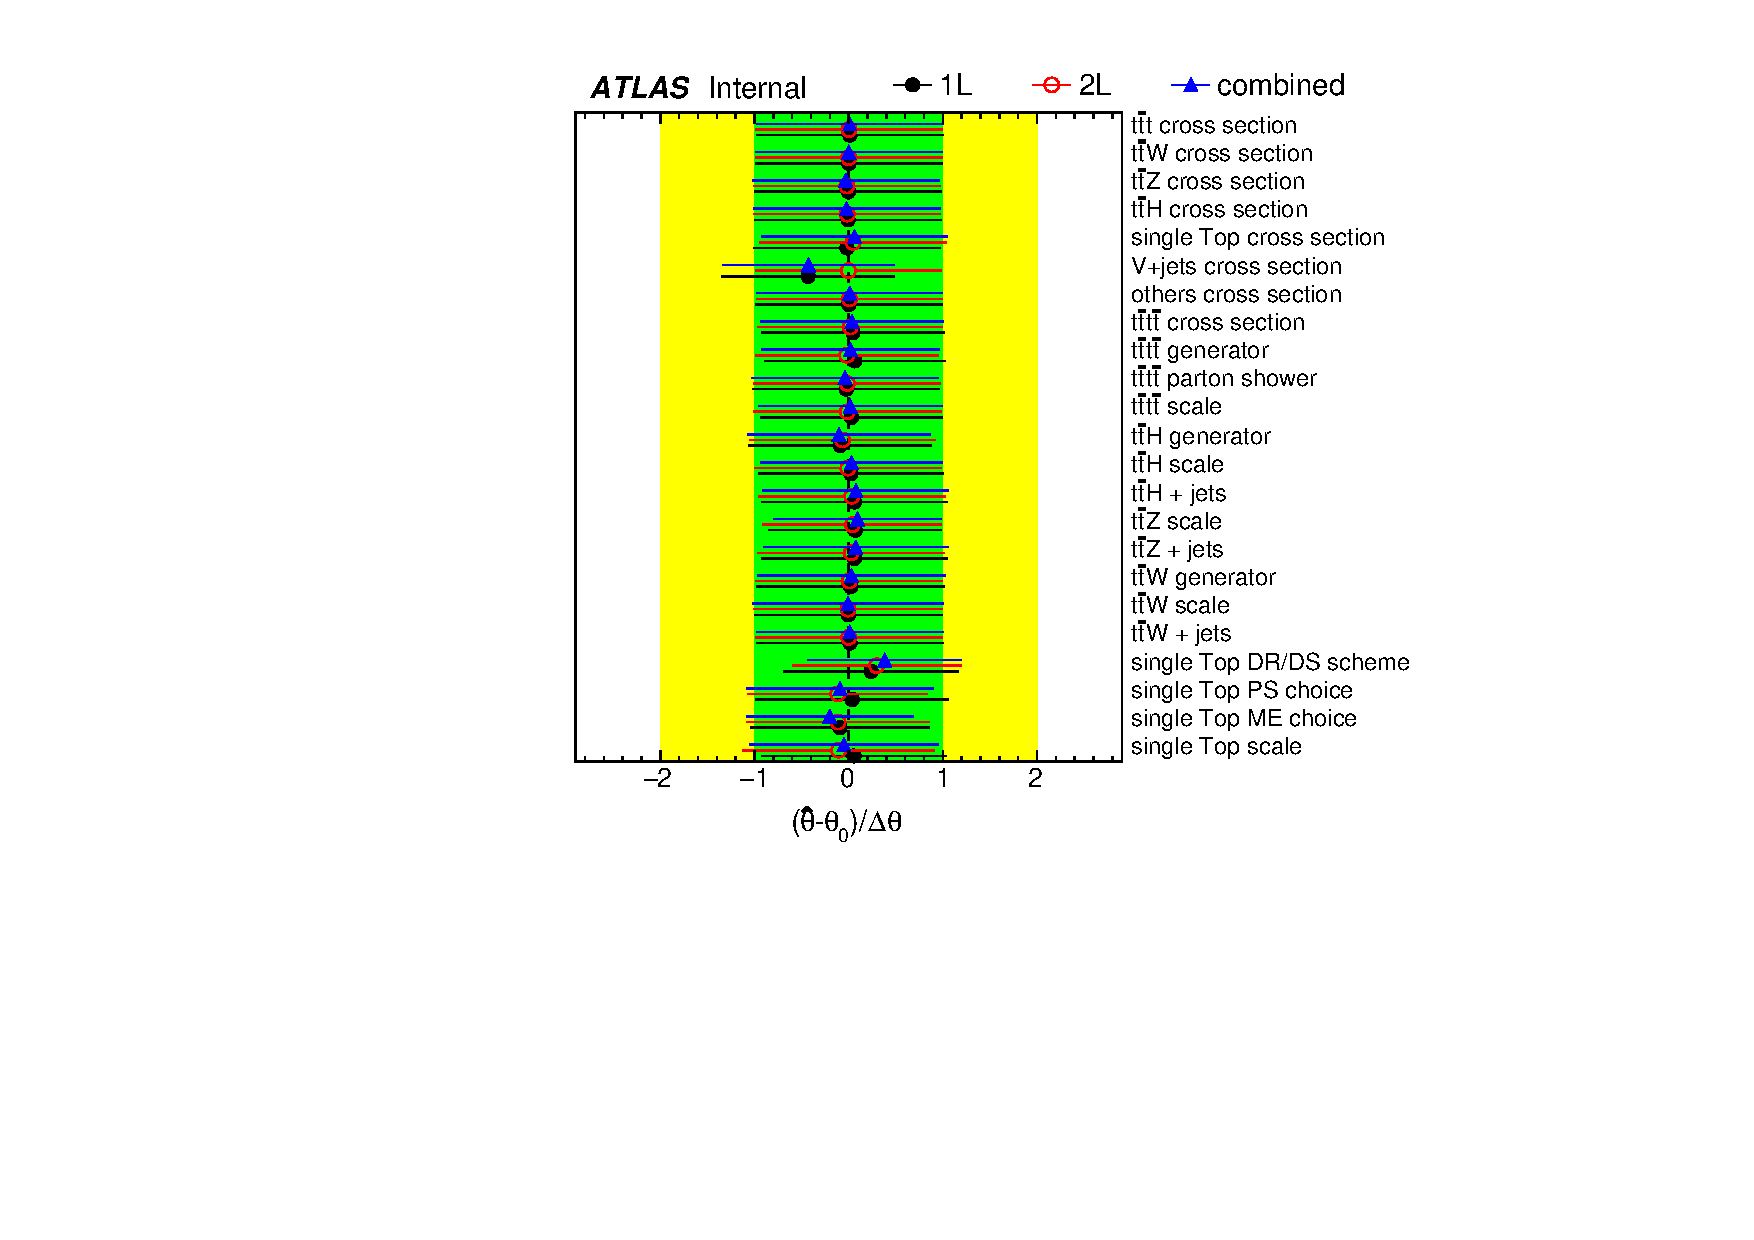
\includegraphics[width=\linewidth]{figures/fits/comparisons/selections/GNN/1000/data_unblindedBonly/NuisPar_comp_Other.pdf}
    \subcaption{mH=1000\gev}
    \label{fig:unblinded_data_Bonly_NP_mH400}
  \end{subfigure}
  \caption{\label{fig:unblinded_data_Bonly_NP_other}Fitted pulls and constraints for the  nuisance parameters corresponding to the non-\ttbar-background systematic uncertainties for the background-only unblinded Data fit for three mass points. Comparison is done for three fits: using only 1L regions, using only 2LOS regions and using all regions.}
\end{figure}



\begin{figure}[htbp!]
  \centering
  \begin{subfigure}[t]{0.32\textwidth}
    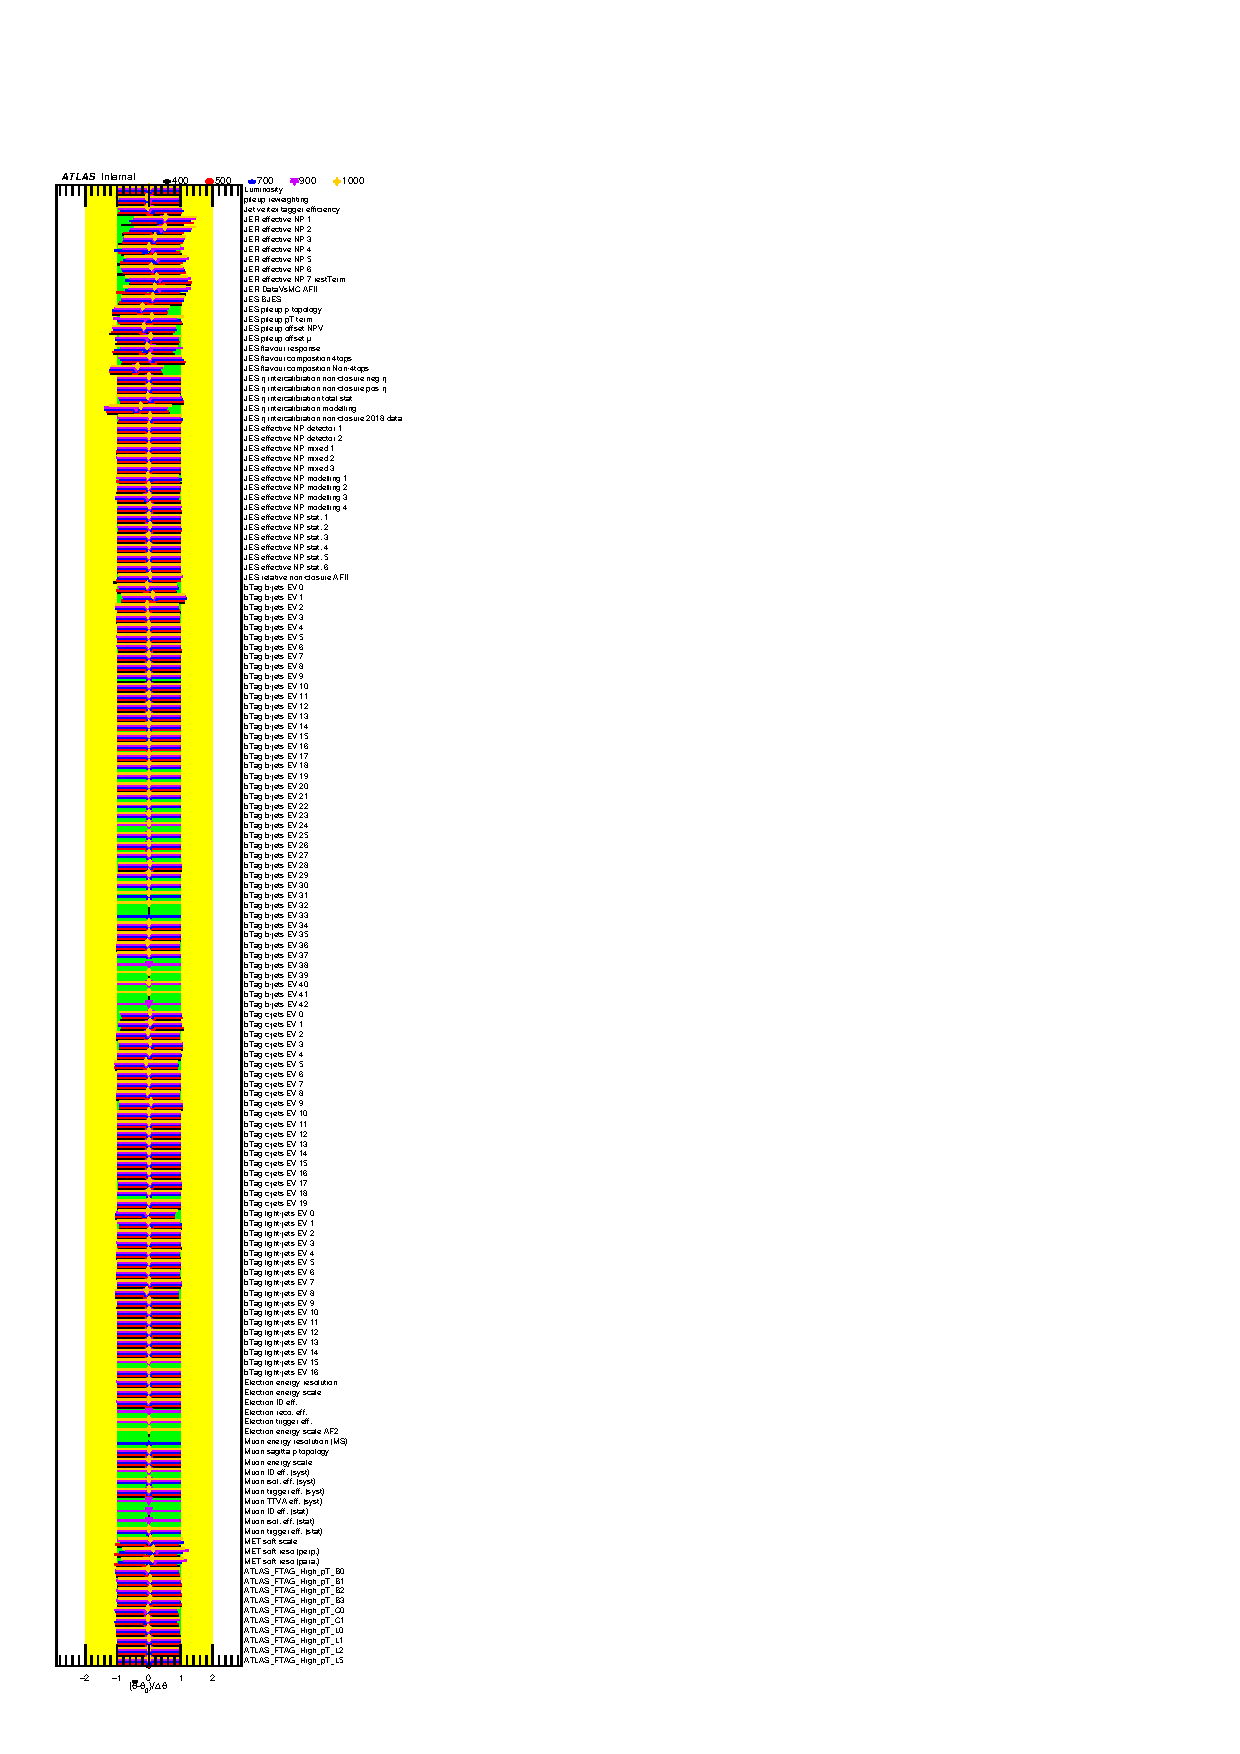
\includegraphics[width=\linewidth]{figures/fits/comparisons/massPoints/GNN/1L/data_unblindedBonly/NuisPar_comp_Instrumental.pdf}
    \subcaption{1L}
    \label{fig:unblinded_data_Bonly_NP_1L_instrumental}
  \end{subfigure}
  \begin{subfigure}[t]{0.32\textwidth}
    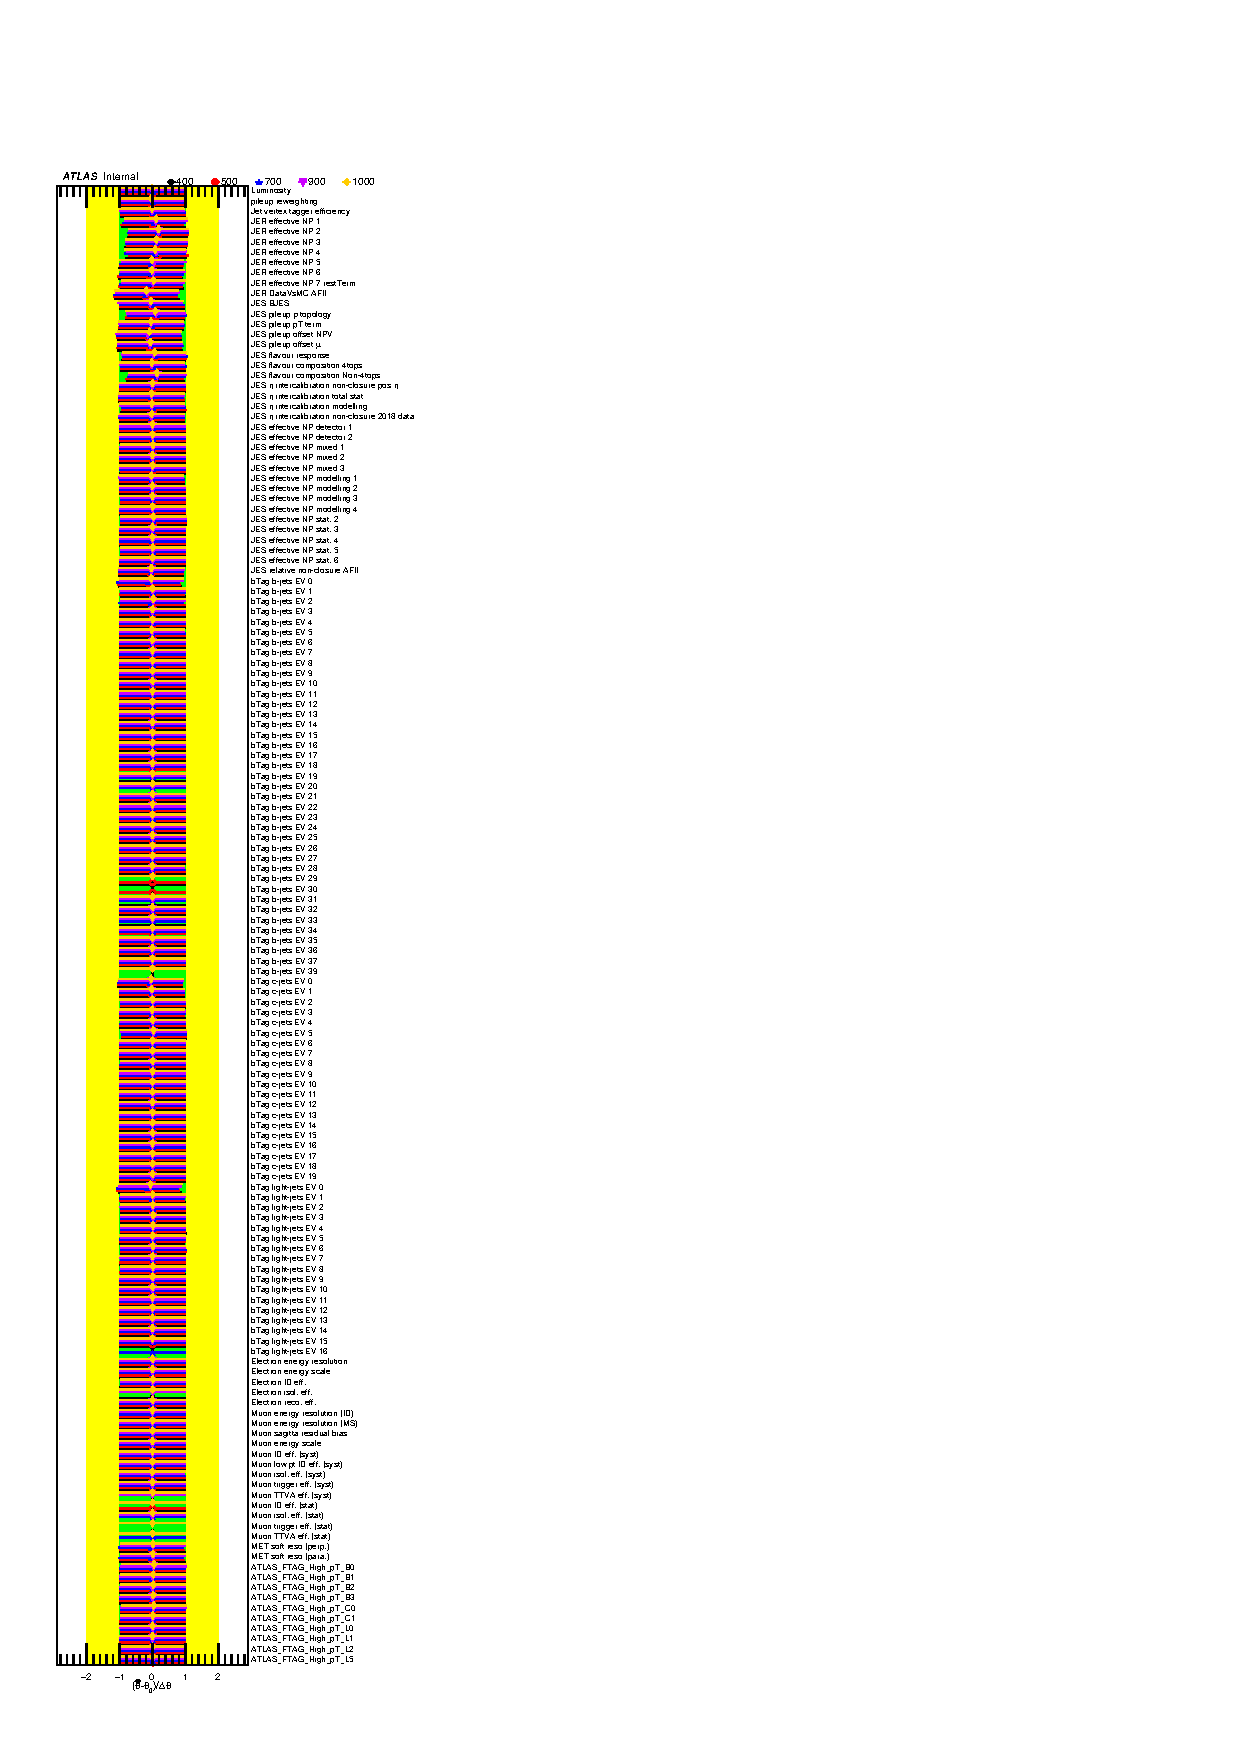
\includegraphics[width=\linewidth]{figures/fits/comparisons/massPoints/GNN/2L/data_unblindedBonly/NuisPar_comp_Instrumental.pdf}
    \subcaption{2L}
    \label{fig:unblinded_data_Bonly_NP_2L_instrumental}
  \end{subfigure}
  \begin{subfigure}[t]{0.32\textwidth}
    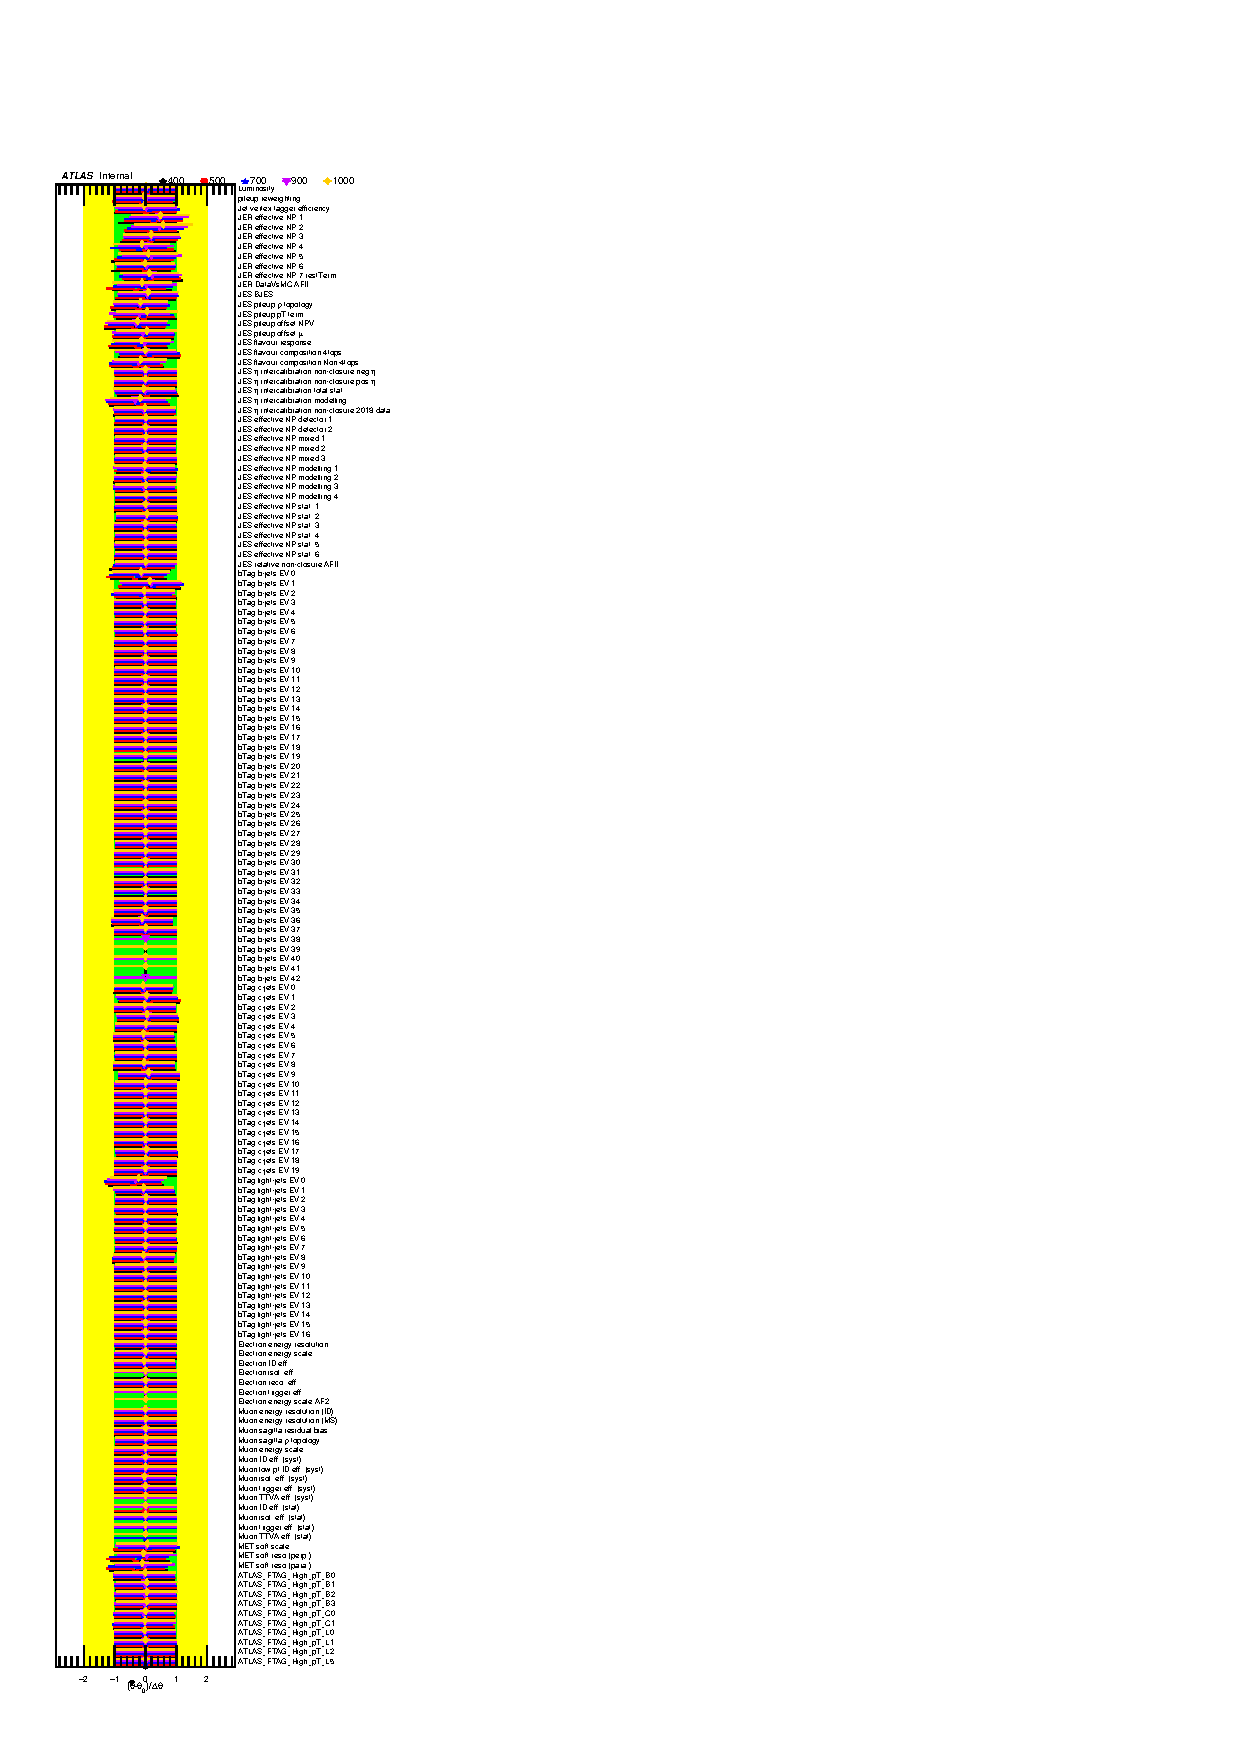
\includegraphics[width=\linewidth]{figures/fits/comparisons/massPoints/GNN/all/data_unblindedBonly/NuisPar_comp_Instrumental.pdf}
    \subcaption{1L+2L}
    \label{fig:unblinded_data_Bonly_NP_all_instrumental}
  \end{subfigure}
  \caption{Fitted pulls and constraints for the nuisance parameters corresponding to the instrumental systematic uncertainties for the background-only unblinded Data fit for three types of fits: using only 1L regions, using only 2L regions, and using all regions. Comparison is done for five mass points.}
\label{fig:unblinded_data_Bonly_NP_mass_instrumental}
\end{figure}


\begin{figure}[htbp!]
  \centering
  \begin{subfigure}[t]{0.32\textwidth}
    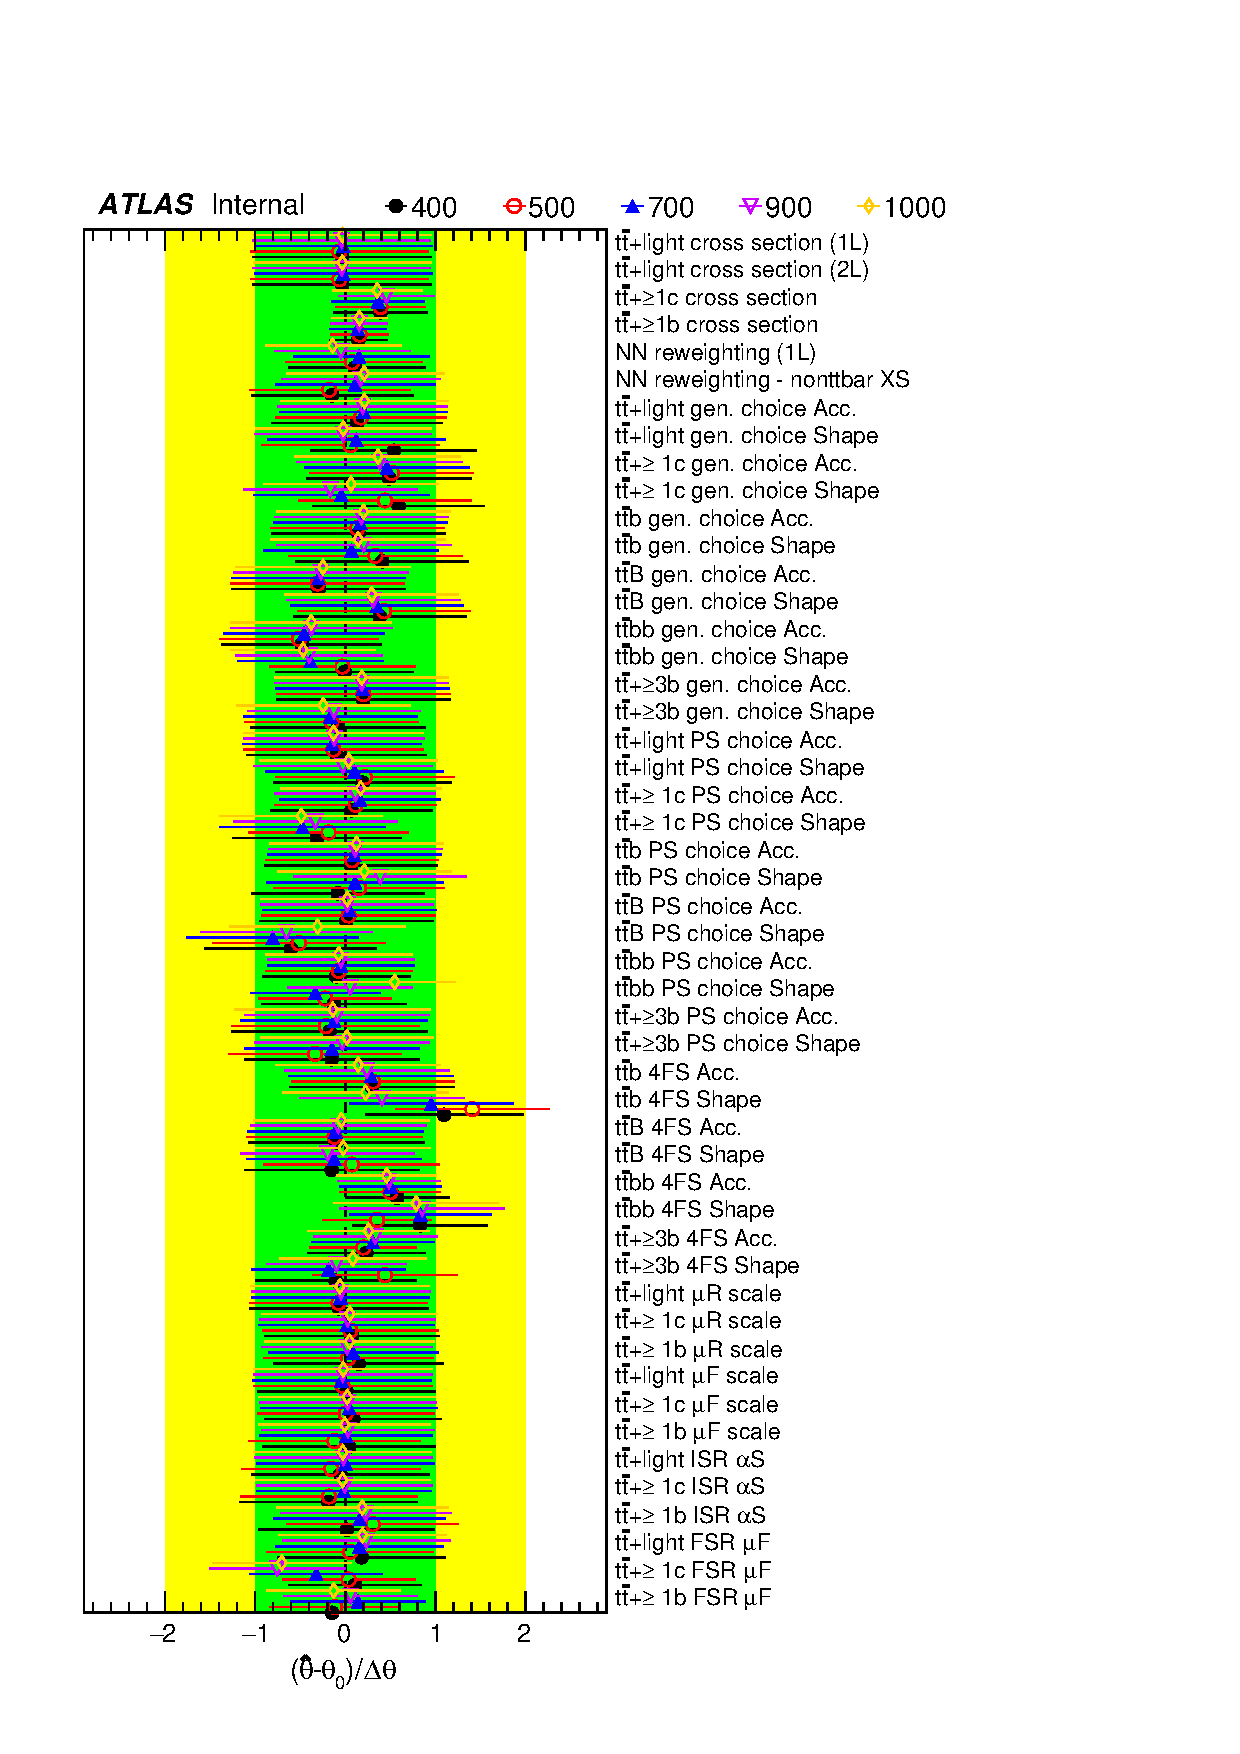
\includegraphics[width=\linewidth]{figures/fits/comparisons/massPoints/GNN/1L/data_unblindedBonly/NuisPar_comp_ttbar.pdf}
    \subcaption{1L}
    \label{fig:unblinded_data_Bonly_NP_1L}
  \end{subfigure}
  \begin{subfigure}[t]{0.32\textwidth}
    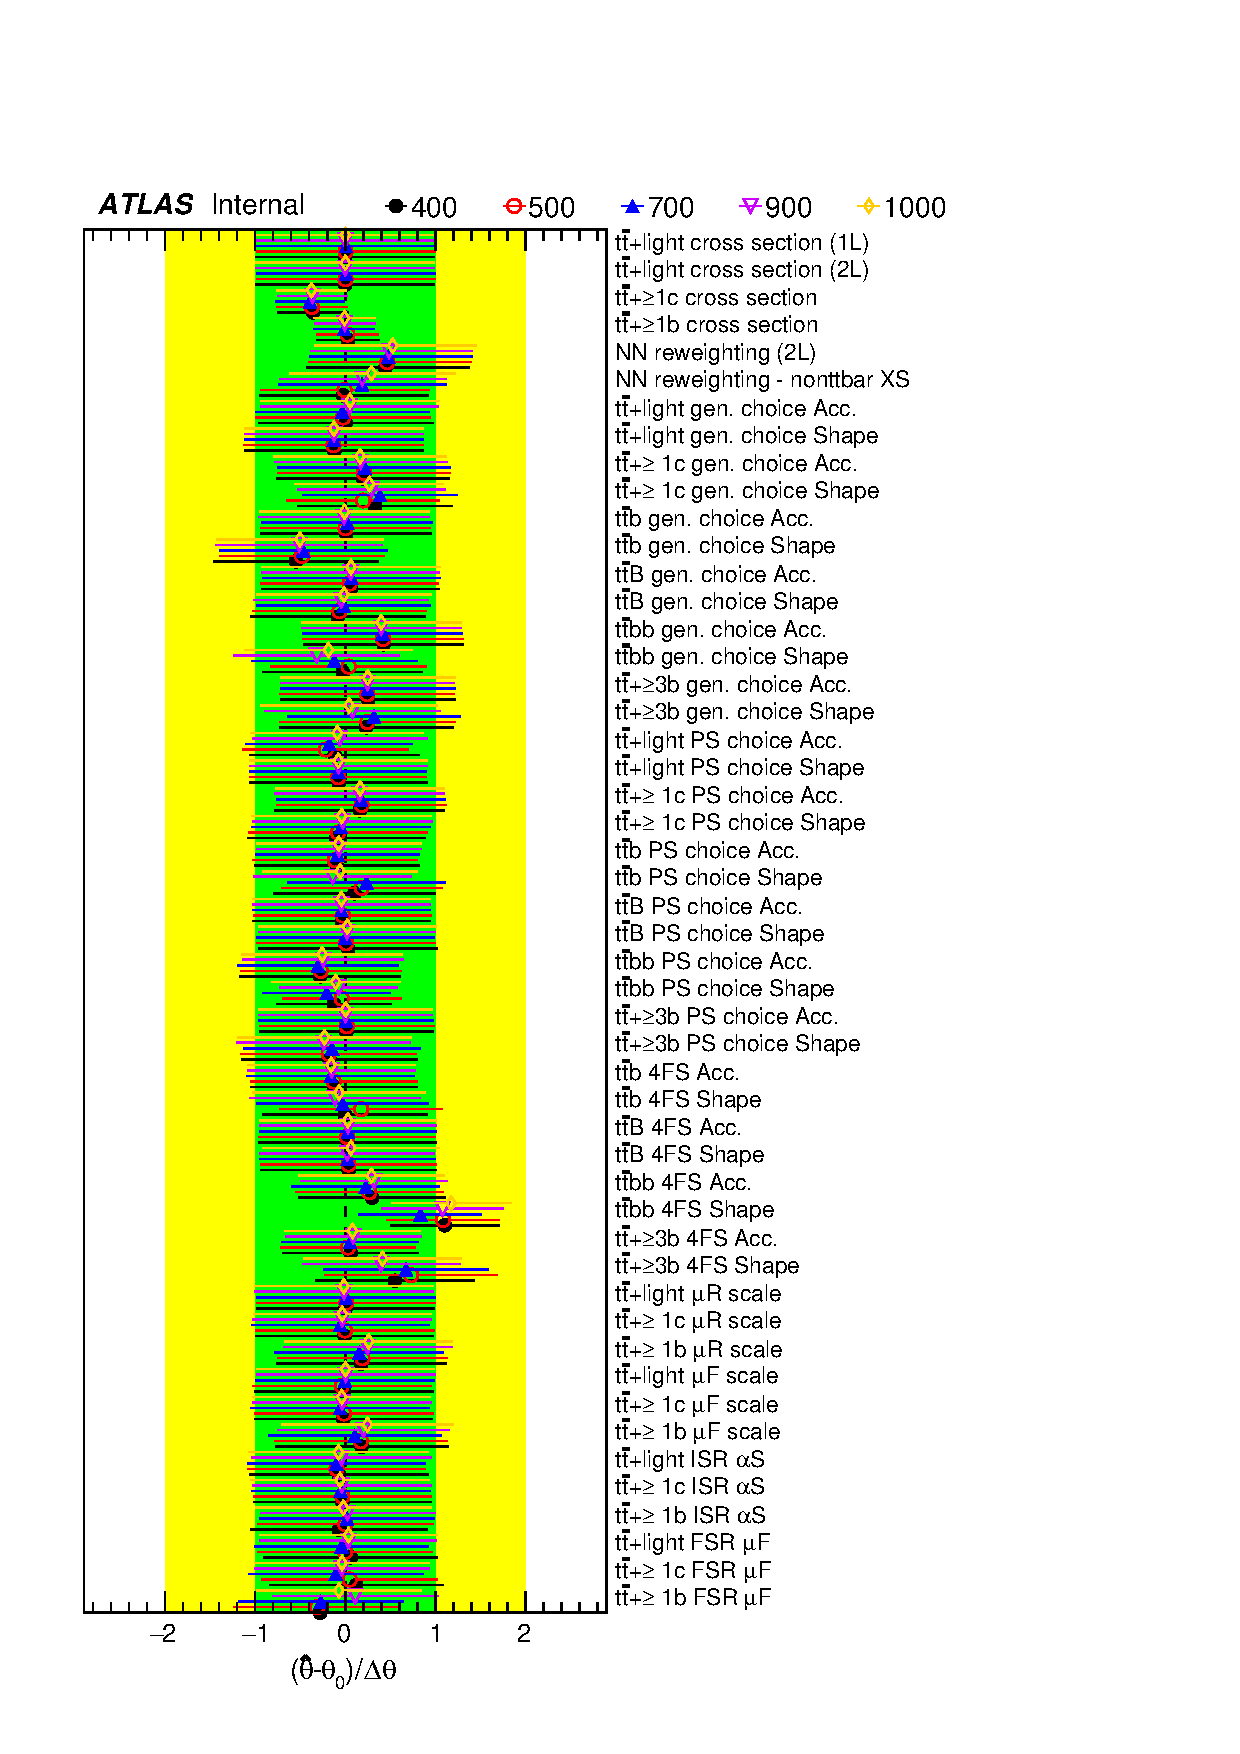
\includegraphics[width=\linewidth]{figures/fits/comparisons/massPoints/GNN/2L/data_unblindedBonly/NuisPar_comp_ttbar.pdf}
    \subcaption{2L}
    \label{fig:unblinded_data_Bonly_NP_2L}
  \end{subfigure}
  \begin{subfigure}[t]{0.32\textwidth}
    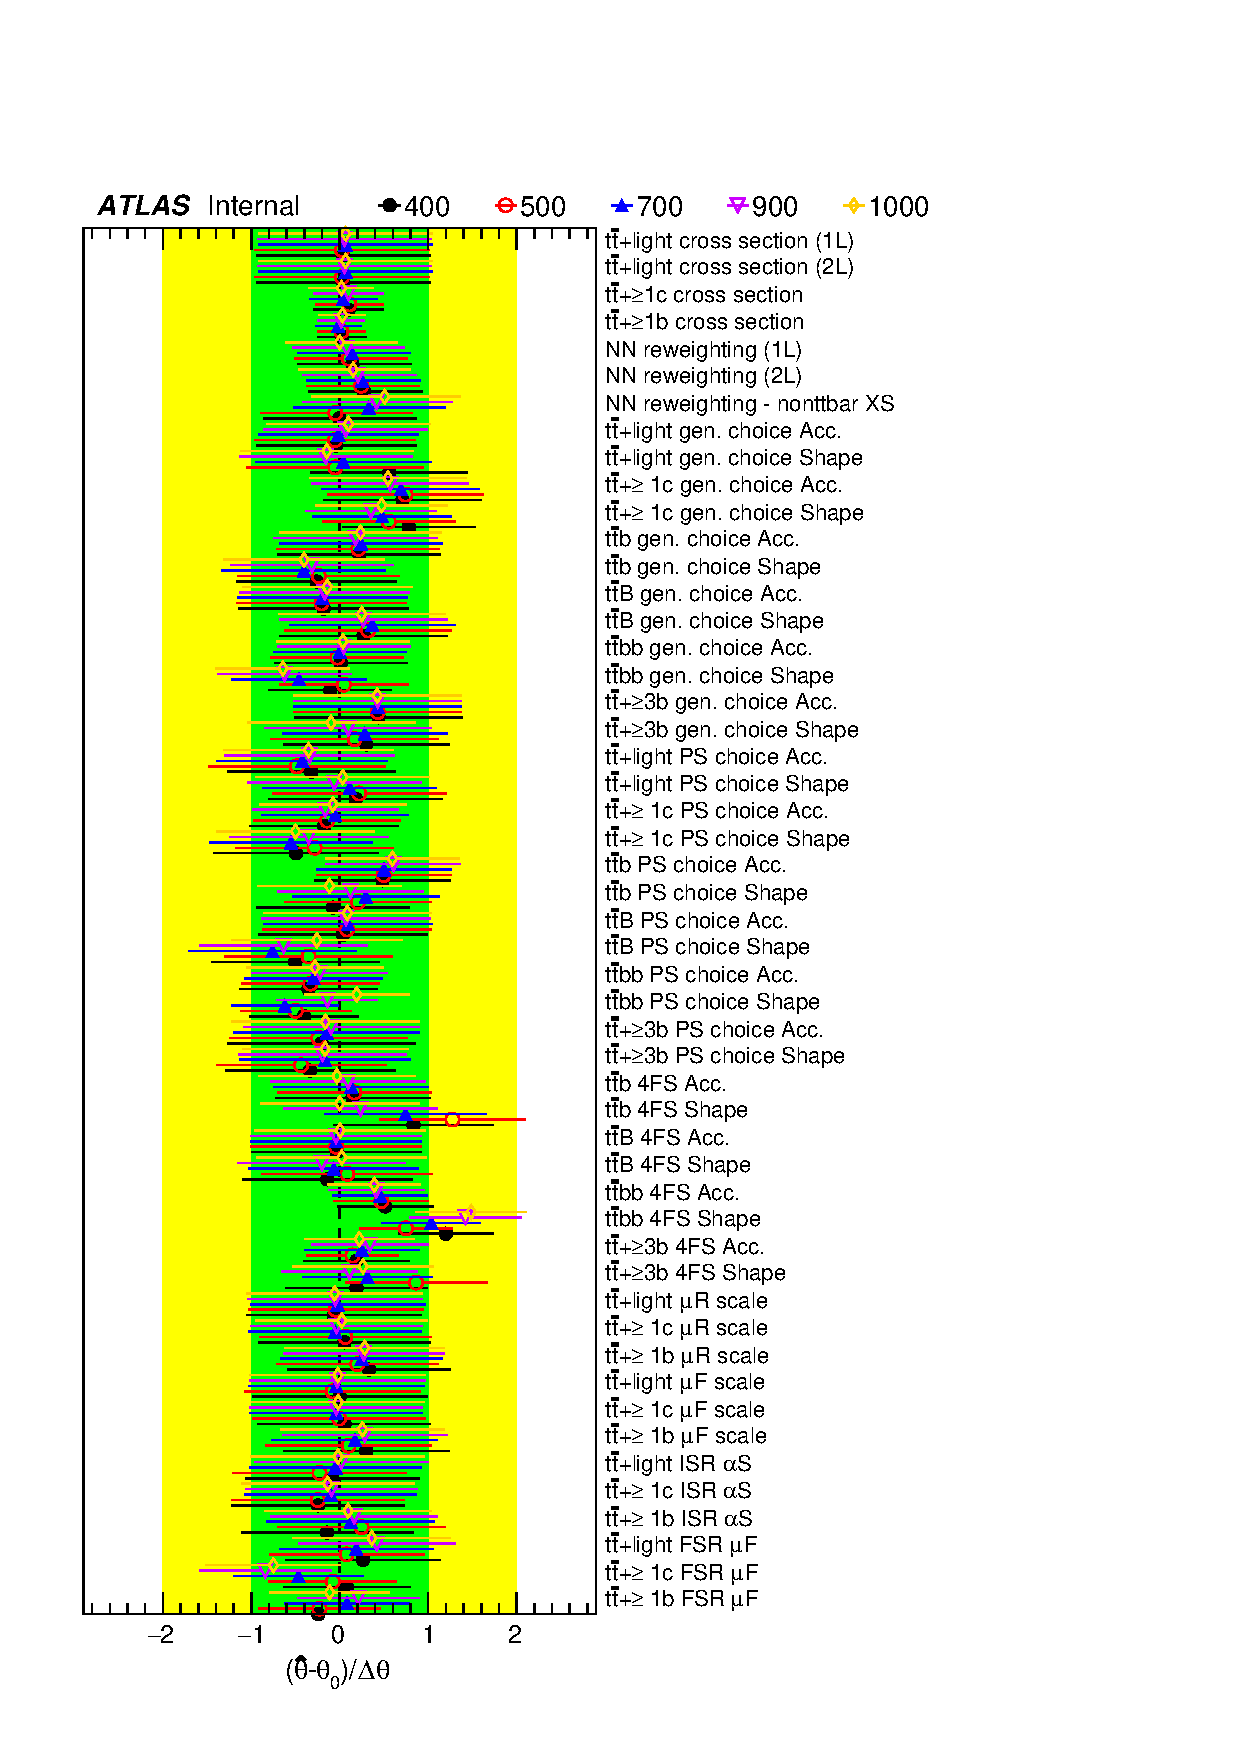
\includegraphics[width=\linewidth]{figures/fits/comparisons/massPoints/GNN/all/data_unblindedBonly/NuisPar_comp_ttbar.pdf}
    \subcaption{1L+2L}
    \label{fig:unblinded_data_Bonly_NP_all}
  \end{subfigure}
  \caption{Fitted pulls and constraints for the nuisance parameters corresponding to the \ttbar systematic uncertainties for the background-only unblinded Data fit for three types of fits: using only 1L regions, using only 2L regions, and using all regions. Comparison is done for five mass points.}
\label{fig:unblinded_data_Bonly_NP_mass_ttbar}
\end{figure}


\begin{figure}[htbp!]
  \centering
  \begin{subfigure}[t]{0.32\textwidth}
    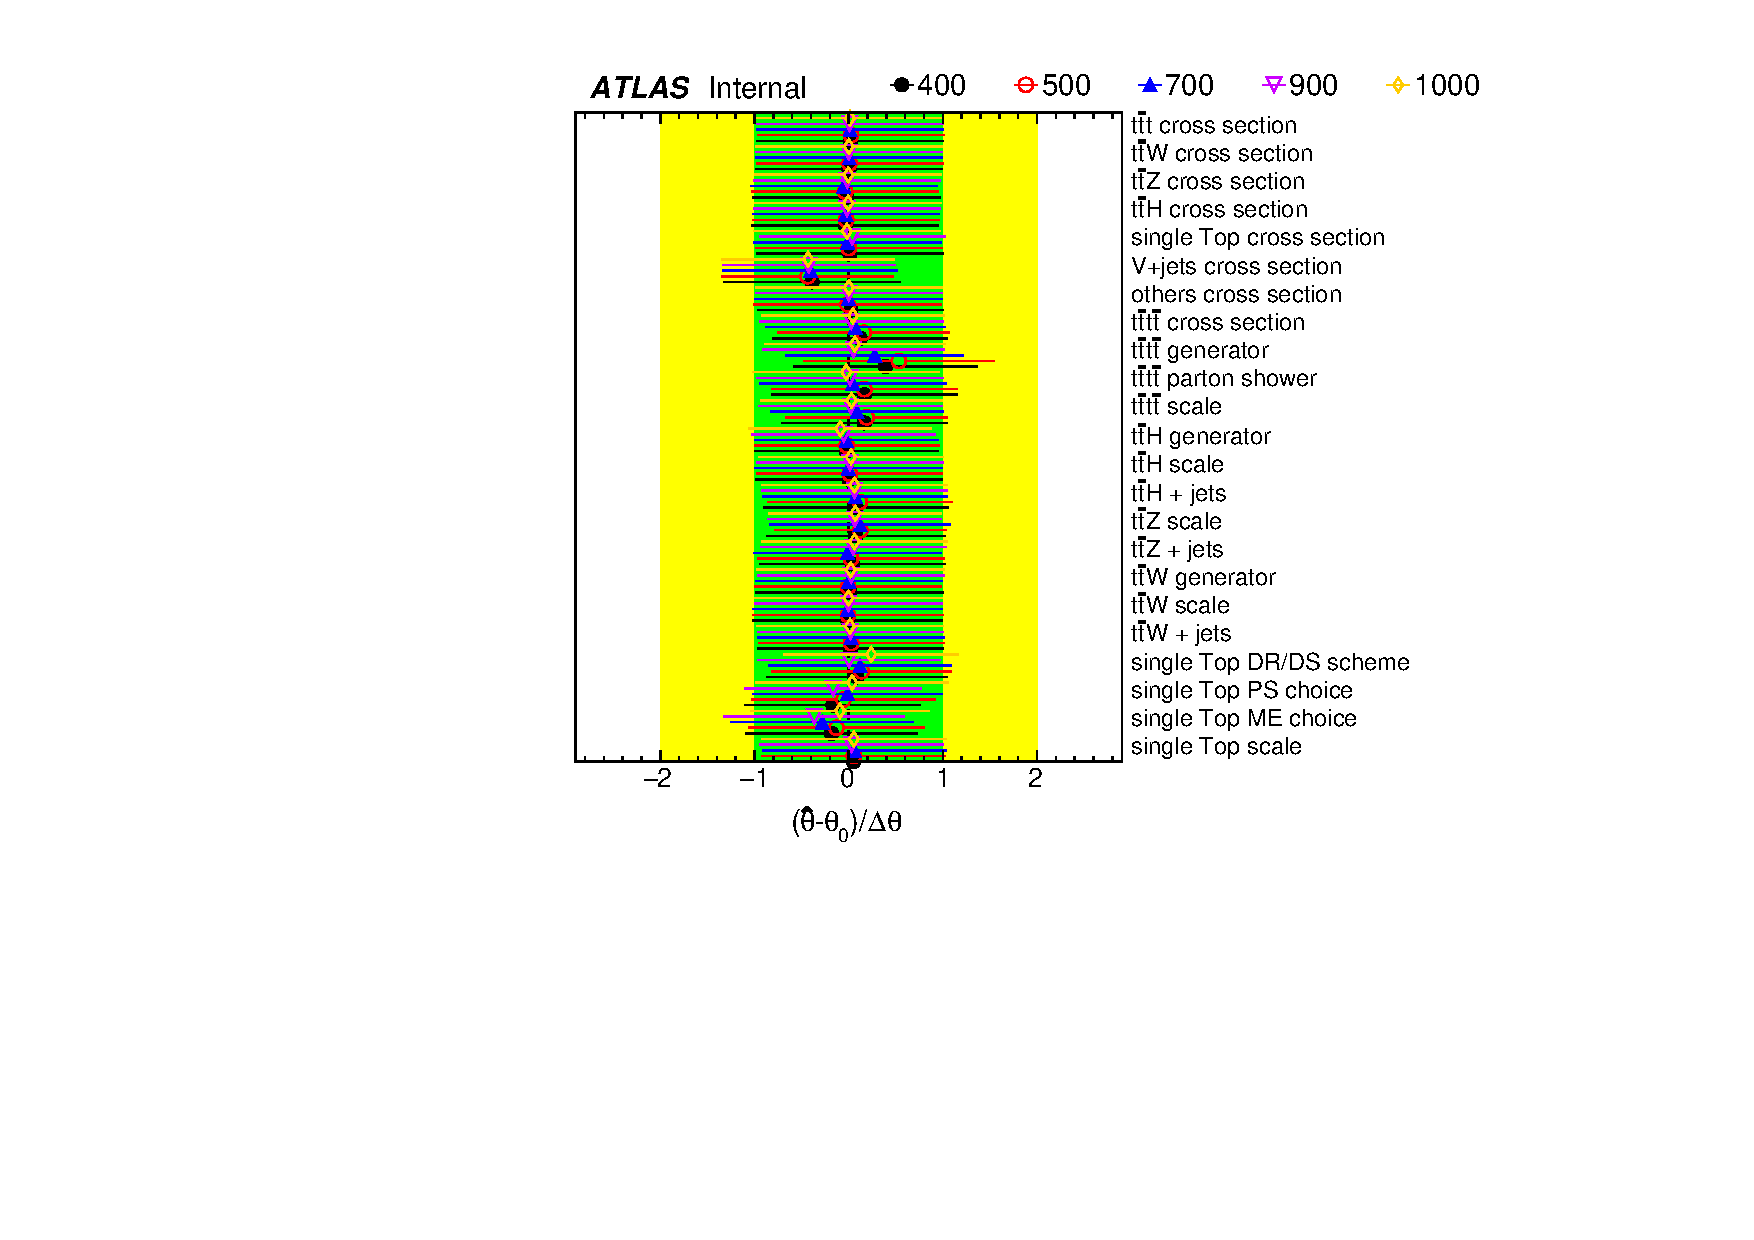
\includegraphics[width=\linewidth]{figures/fits/comparisons/massPoints/GNN/1L/data_unblindedBonly/NuisPar_comp_Other.pdf}
    \subcaption{1L}
    \label{fig:unblinded_data_Bonly_NP_1L_other}
  \end{subfigure}
  \begin{subfigure}[t]{0.32\textwidth}
    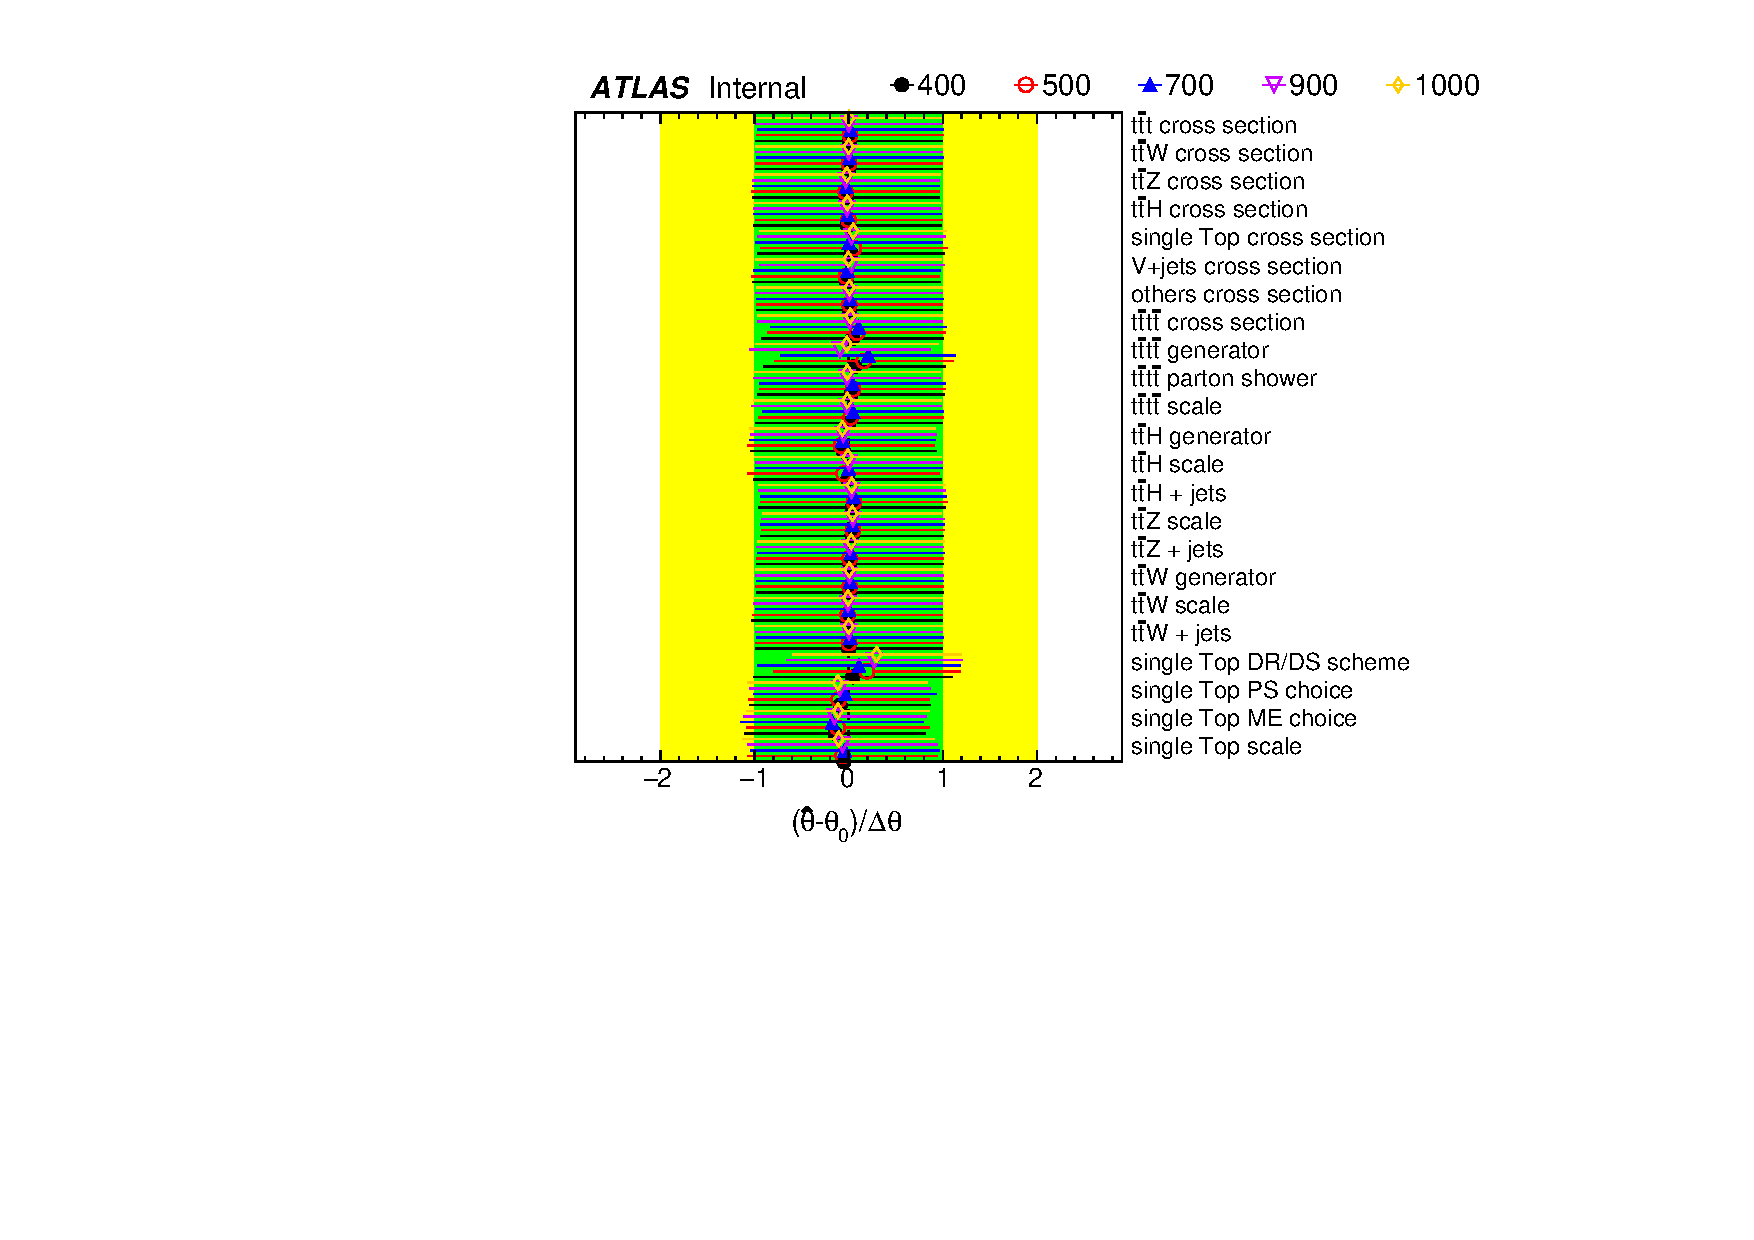
\includegraphics[width=\linewidth]{figures/fits/comparisons/massPoints/GNN/2L/data_unblindedBonly/NuisPar_comp_Other.pdf}
    \subcaption{2L}
    \label{fig:unblinded_data_Bonly_NP_2L_other}
  \end{subfigure}
  \begin{subfigure}[t]{0.32\textwidth}
    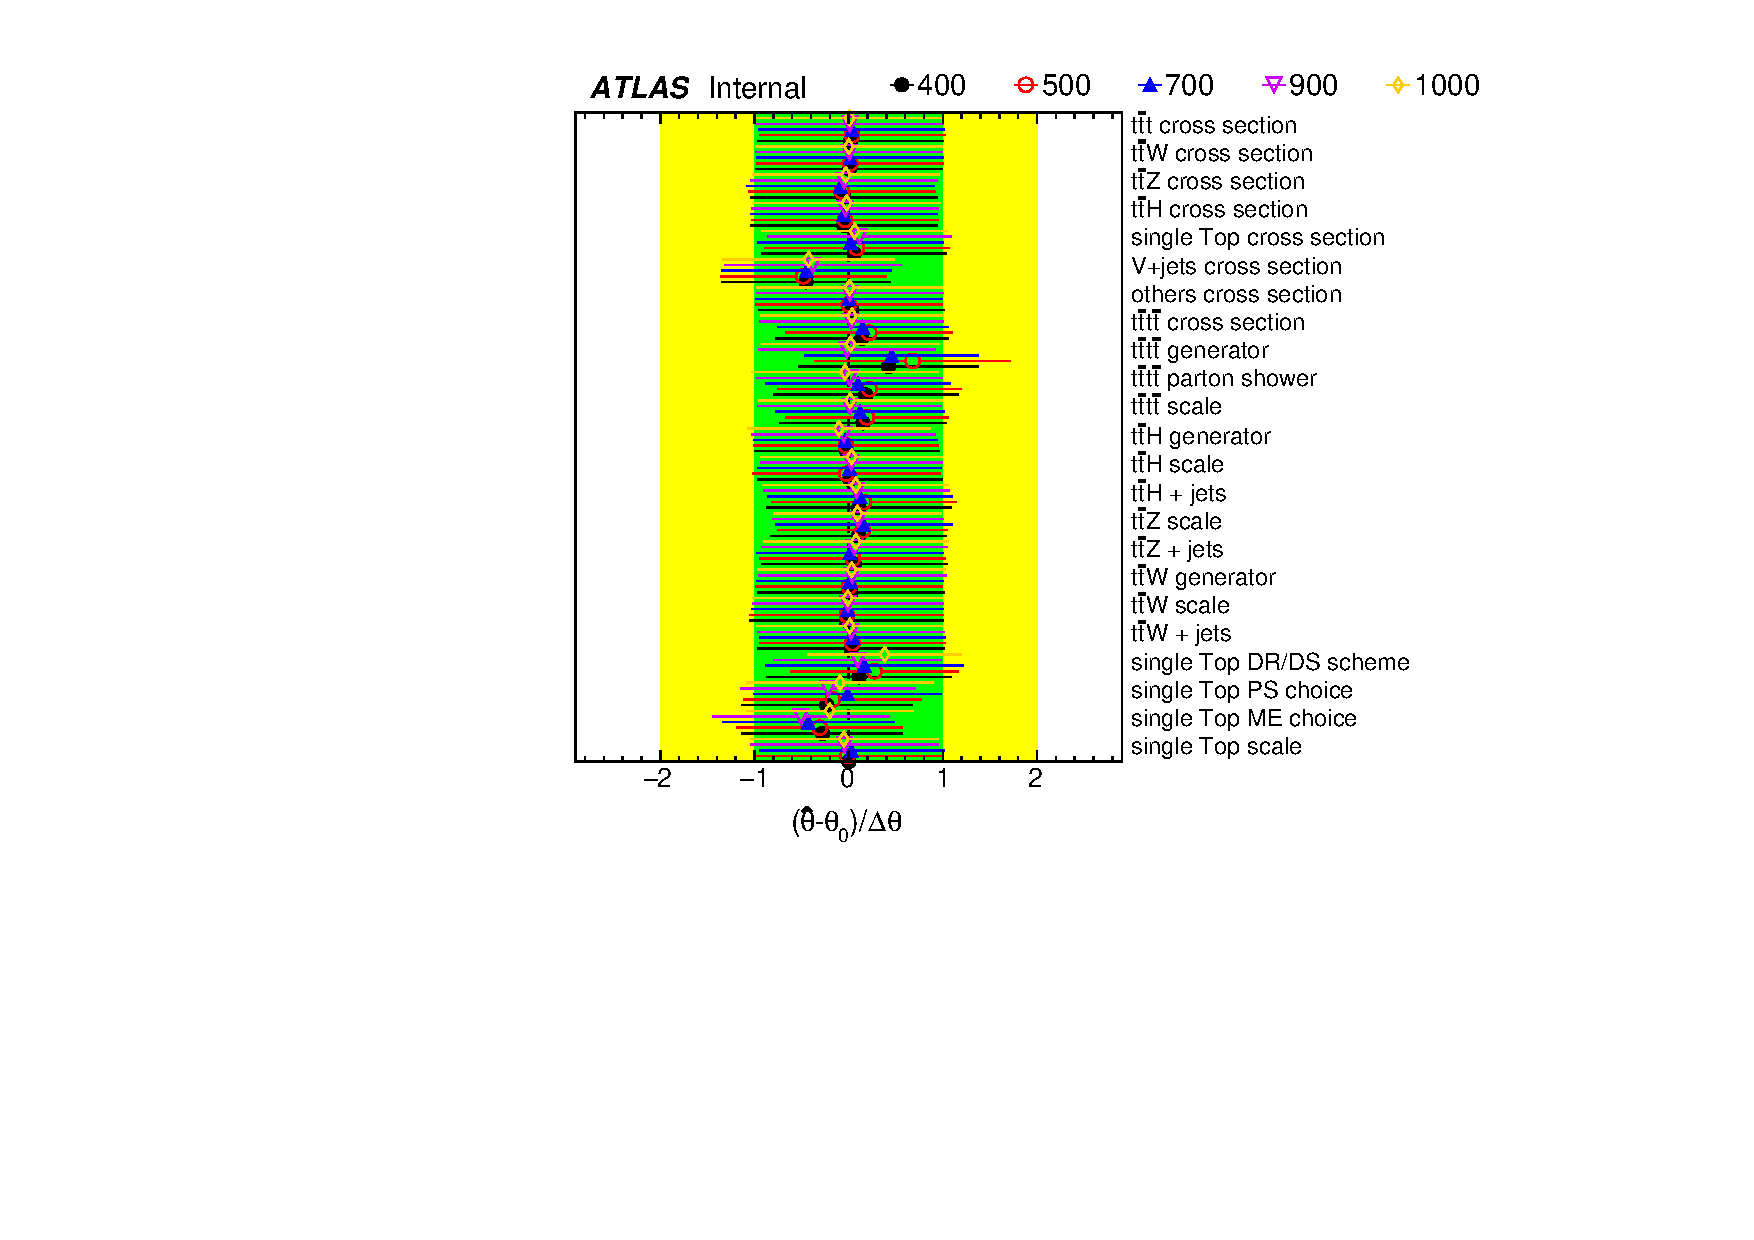
\includegraphics[width=\linewidth]{figures/fits/comparisons/massPoints/GNN/all/data_unblindedBonly/NuisPar_comp_Other.pdf}
    \subcaption{1L+2L}
    \label{fig:unblinded_data_Bonly_NP_all_other}
  \end{subfigure}
  \caption{Fitted pulls and constraints for the nuisance parameters corresponding to the non-\ttbar-background systematic uncertainties for the background-only unblinded Data fit for three types of fits: using only 1L regions, using only 2L regions, and using all regions. Comparison is done for five mass points.}
\label{fig:unblinded_data_Bonly_NP_mass_other}
\end{figure}


\begin{figure}[htbp!]
        \centering
        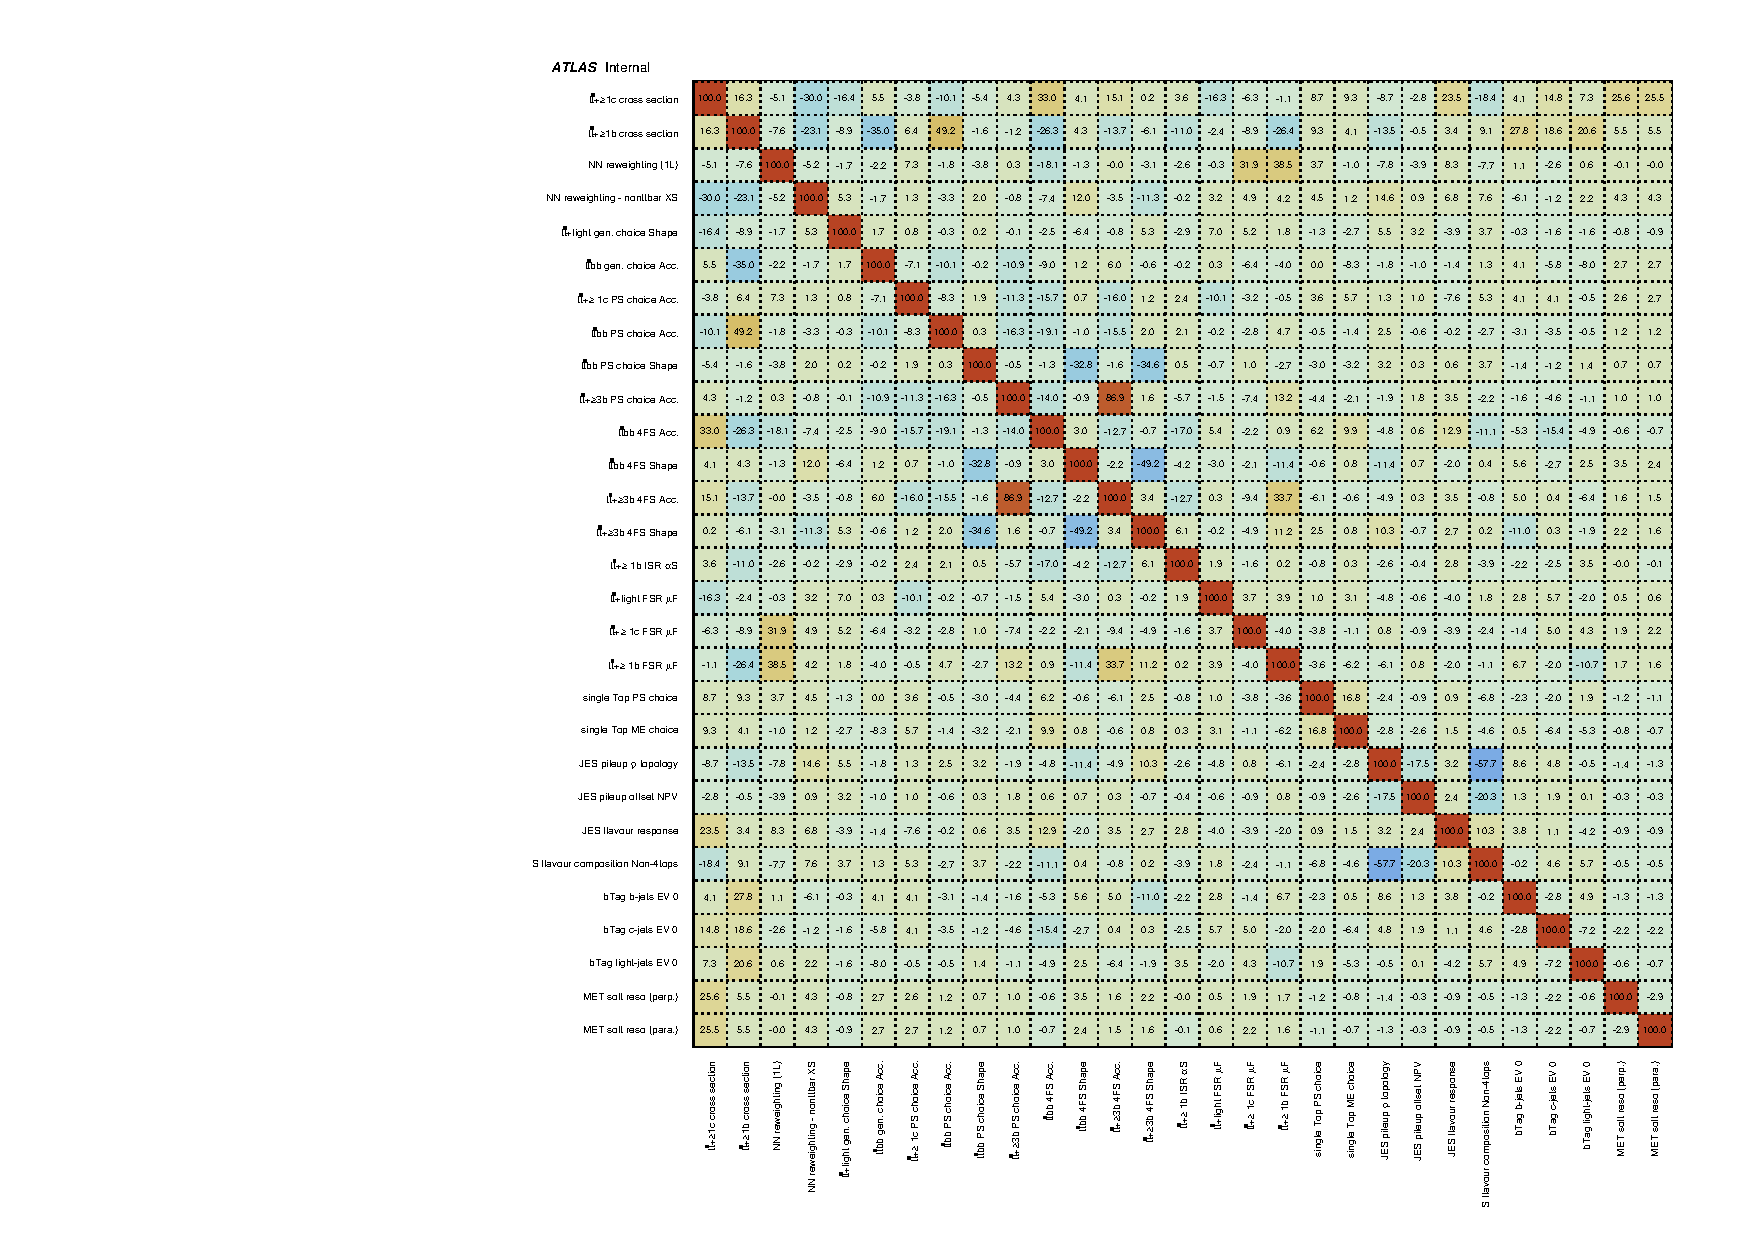
\includegraphics[width=\linewidth]{figures/fits/GNN/400/1L/data_unblindedBonly/CorrMatrix.pdf}
        \caption{\label{fig:unblinded_data_Bonly_corr_mH400_Data_1L}Correlation matrix for the 1L unblinded data fit for mH = 400 GeV}
\end{figure}

\begin{figure}[htbp!]
        \centering
        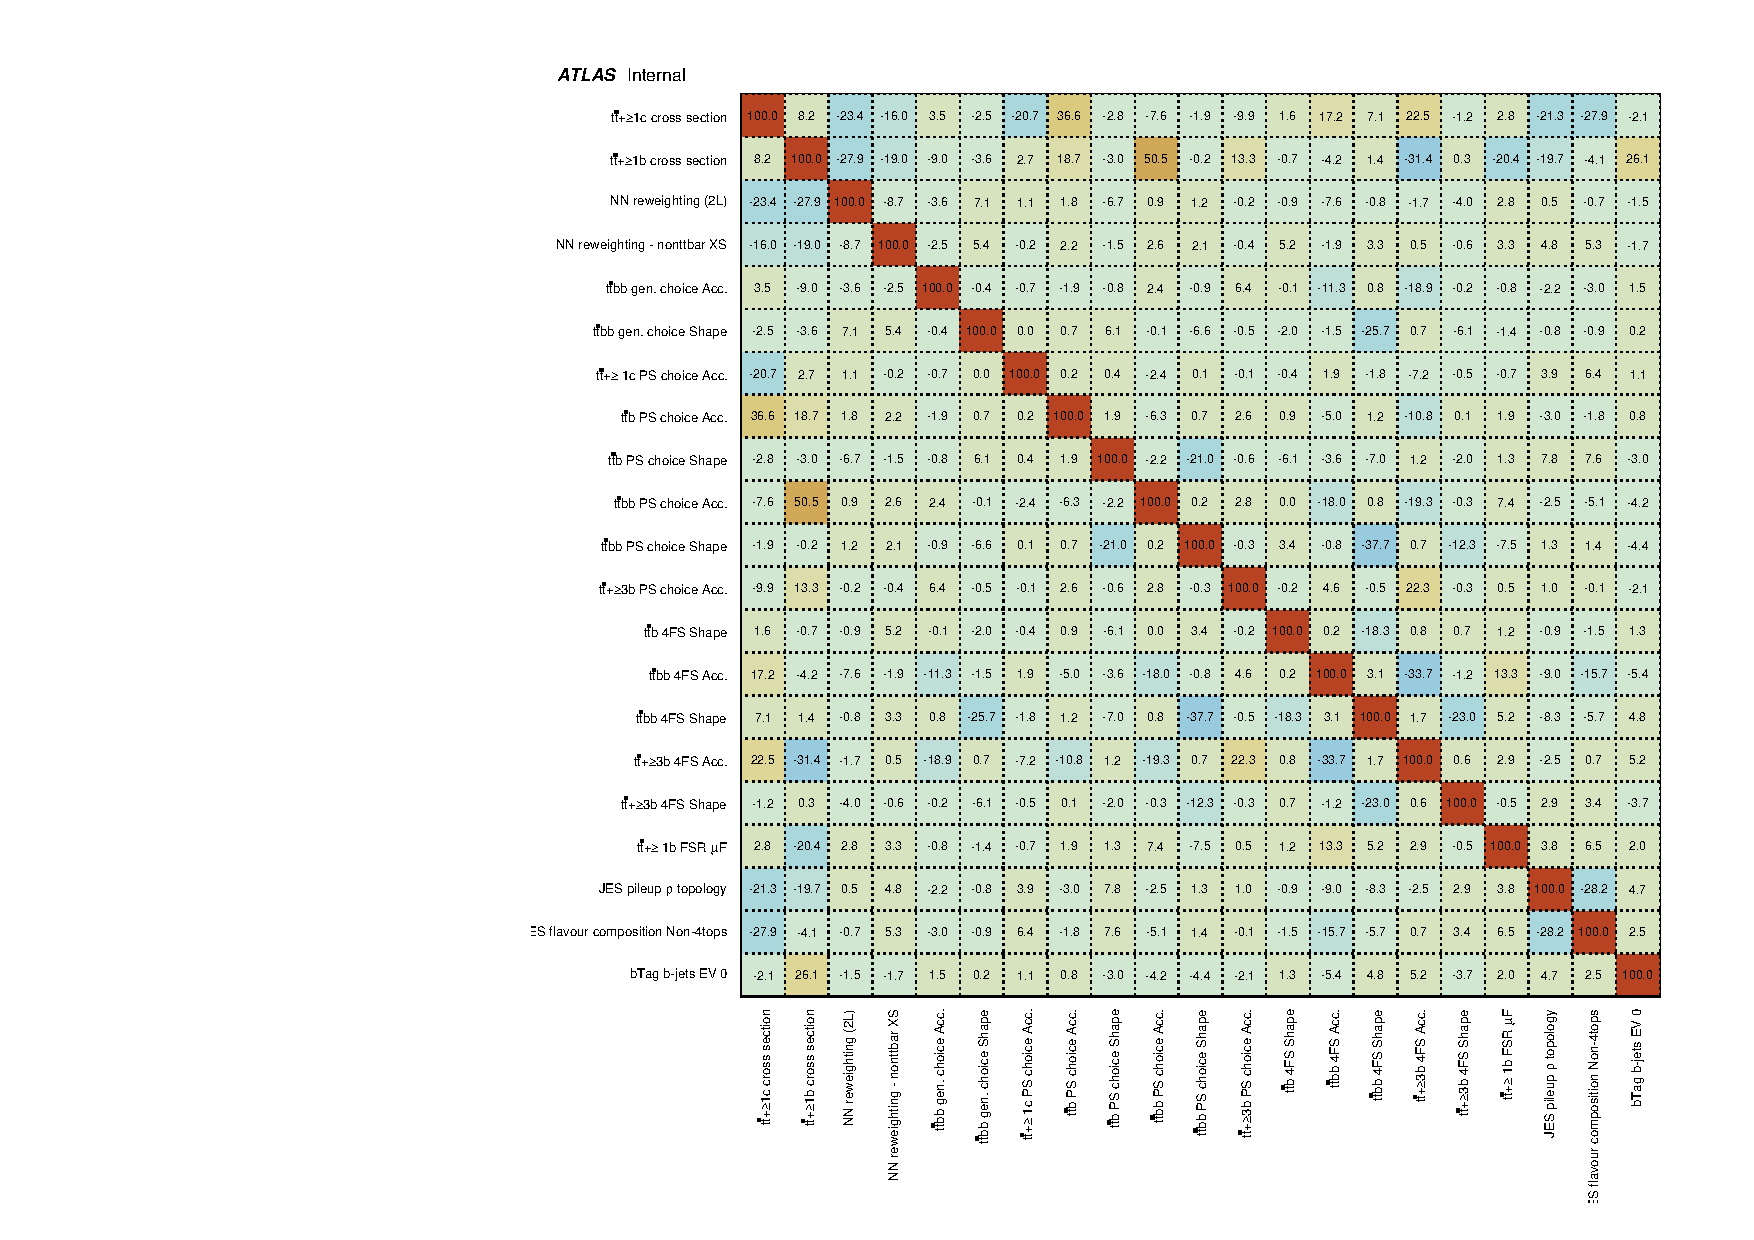
\includegraphics[width=\linewidth]{figures/fits/GNN/400/2L/data_unblindedBonly/CorrMatrix.pdf}
        \caption{\label{fig:unblinded_data_Bonly_corr_mH400_Data_2L}Correlation matrix for the 2LOS unblinded data fit for mH = 400 GeV}
\end{figure}

\begin{figure}[htbp!]
        \centering
        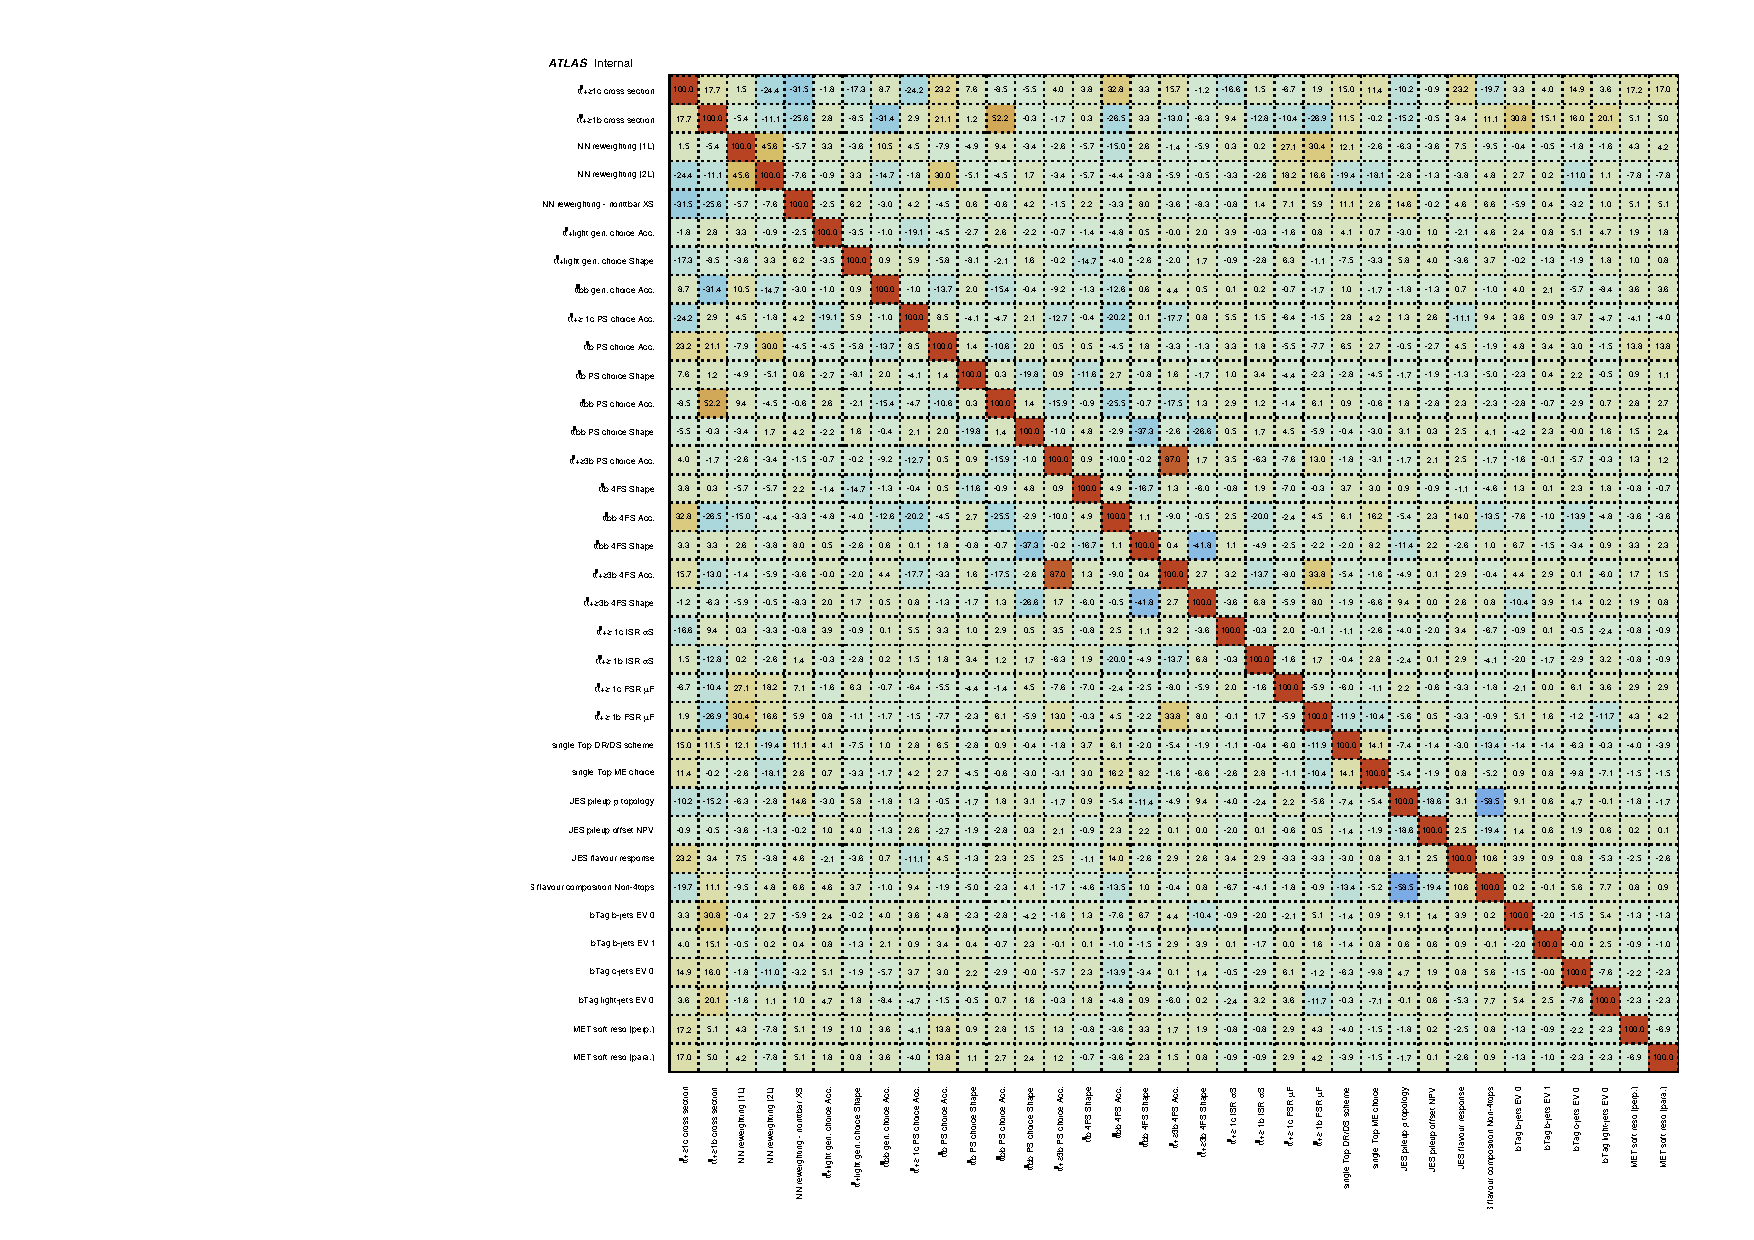
\includegraphics[width=\linewidth]{figures/fits/GNN/400/all/data_unblindedBonly/CorrMatrix.pdf}
        \caption{\label{fig:unblinded_data_Bonly_corr_mH400_Data_all}Correlation matrix for the 1L/2LOS combined unblinded data fit for mH = 400 GeV}
\end{figure}




\begin{figure}[htbp!]
  \centering
  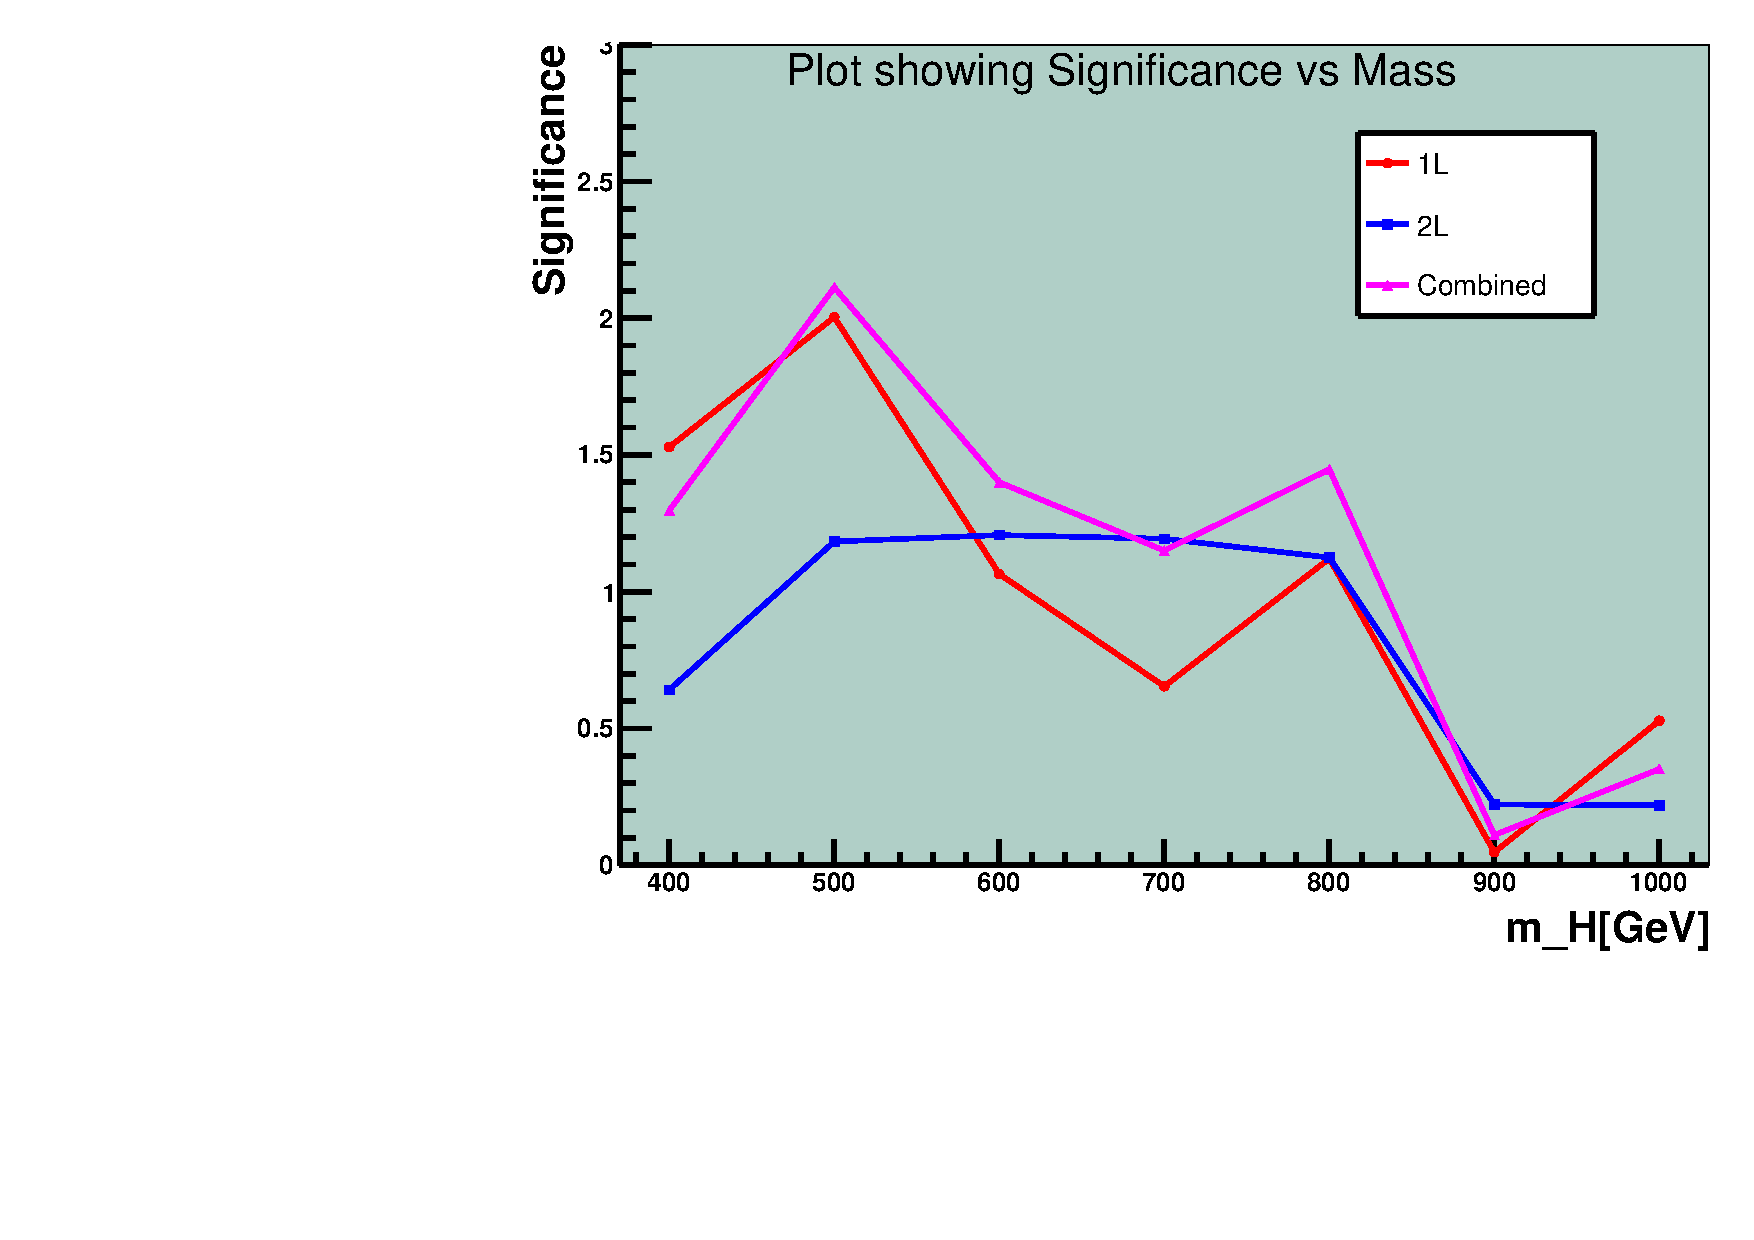
\includegraphics[width=0.4 \textwidth]{figures/fits/significanceVsMass.pdf}
  \caption{\label{fig:data_Bonly_significance}Comparison of the observed significance.}
\end{figure}


